% file: main.tex

\documentclass[10pt,a4paper,oneside]{article}
\usepackage{setspace}
%\usepackage[ngerman]{babel}
\usepackage[utf8]{inputenc}
\usepackage{fancyhdr}
\usepackage{tabularx}
%\renewcommand{\rmdefault}{phv}
%\renewcommand{\sfdefault}{phv}
\usepackage[a4paper,left=2cm,right=2cm,top=2cm,bottom=2cm]{geometry}
\onehalfspacing

\setcounter{tocdepth}{2} % to get subsubsections in toc 
% cf. http://www.latex-community.org/forum/viewtopic.php?f=47&p=44760

\usepackage{amssymb,latexsym}
\usepackage{amsmath, amsthm}

%for bibliography; installation using 'sudo tlmgr install amsrefs'
\usepackage{amsrefs}

\usepackage{graphics}

\usepackage{hyperref}
\hypersetup{colorlinks=true, urlcolor=blue}

\usepackage{cancel} % http://jansoehlke.com/2010/06/strikethrough-in-latex/

\usepackage{listings} % http://en.wikibooks.org/wiki/LaTeX/Source_Code_Listings
% http://olmjo.com/files/teaching/PSC505/LaTeXandR.pdf

% package for flower symbol (\ding(96))
\usepackage{pifont}
% required installation: sudo apt-get install texlive-fonts-recommended (30MB)
% http://tug.ctan.org/info/symbols/comprehensive/symbols-a4.pdf

\usepackage{tikz} % for diagrams
\usetikzlibrary{matrix,positioning,arrows,calc,decorations.pathmorphing,shapes}
% for snaky lines (http://tex.stackexchange.com/questions/209942/curved-arrows-in-tikz) 
\tikzset{snake it/.style={-stealth,
decoration={snake, 
    amplitude = .4mm,
    segment length = 2mm,
    post length=0.9mm},decorate}}

\usepackage[parfill]{parskip}

\usepackage{framed} %for putting some text in boxes using \begin{framed}

\usepackage{enumerate}

%for displaying tensor indices properly. requires installation of tensor package using 'sudo tlmgr install tensor'
\usepackage{tensor}

%for placing captions of figures on the side instead of above/below the figure
\usepackage{sidecap}
\linespread{1.2}

%plain makes sure that we have page numbers
\pagestyle{plain}

\theoremstyle{plain}
\newtheorem{axiom}{Axiom}
\newtheorem{theorem}{Theorem}
\newtheorem{corollary}{Corollary}
\newtheorem*{main}{Main Theorem}
\newtheorem{lemma}{Lemma}
\newtheorem{proposition}{Proposition}

\theoremstyle{definition}
\newtheorem{definition}{Definition}

\theoremstyle{remark}
\newtheorem*{notation}{Notation}

\numberwithin{equation}{section}
\numberwithin{figure}{section}
\numberwithin{theorem}{section}

%symbol for maps
\renewcommand{\to}{\longrightarrow}
\newcommand{\injmapto}{\hookrightarrow}
\newcommand{\surjmapto}{\twoheadrightarrow}
\newcommand{\linearmapto}{\stackrel{\sim}{\longrightarrow}}
\newcommand{\projmapto}{\stackrel{\pi}{\longrightarrow}}

\newcommand{\after}{\circ}
\newcommand{\stdtop}{\mathcal{O}_{std}}
\newcommand{\cibasis}[2][]{\frac{\partial #1}{\partial #2}}

%connection coefficient functions or gammas
\newcommand{\ccf}[2]{\Gamma\indices{^{#1}_{#2}}}
\newcommand{\ccfx}[3]{\left(\Gamma_{#3}\right)\indices{^{#1}_{#2}}} % with chart index

%set theory symbols
%\renewcommand{\exists}{\exists\,}
%\renewcommand{\forall}{\forall\,}

%This defines a new command \questionhead which takes one argument and prints out Question #. with some space.
\newcommand{\questionhead}[1]
  {
   \noindent{\small\bf Question #1.}
  }

\newcommand{\problemhead}[1]
  {
   \noindent{\small\bf Problem #1.}
  }

\newcommand{\exercisehead}[1]
  { \smallskip
   \noindent{\small\bf Exercise #1.}
  }

\newcommand{\solutionhead}[1]
  {
   \noindent{\small\bf Solution #1.}
  }

%-----------------------------------
\begin{document}

%-----------------------------------

\title{Lecture Notes on General Relativity (GR)}
\author{lazierthanthou \\ (\url{https://github.com/lazierthanthou/Lecture_Notes_GR})}
%\thanks{}
%\keywords{General Relativity, Gravity, Differential Geometry, Manifolds, Integration, mathematics, physics}
\date{\today}

\maketitle

\tableofcontents

\begin{abstract}
These are lecture notes on General Relativity.

They are based on the \href{https://www.youtube.com/channel/UCUHKG3S9N_QeIE2jQXd2-VQ/feed}{Central Lecture Course} by \textbf{Dr. Frederic P. Schuller} (\textbf{A thorough introduction to the theory of general relativity}) introducing the mathematical and physical foundations of the theory in 24 self-contained lectures at the International Winter School on Gravity and Light in Linz/Austria for the WE Heraeus International Winter School of Gravity and Light, 2015 in Linz as part of the world-wide celebrations of the 100th anniversary of Einstein's theory of general relativity and the International Year of Light 2015.

These lectures develop the theory from first principles and aim at an audience ranging from ambitious undergraduate students to beginning PhD students in mathematics and physics. Satellite Lectures (see other videos on this channel) by Bernard F Schutz (Gravitational Waves), Domenico Giulini (Canonical Formulation of Gravity), Marcus C Werner (Gravitational Lensing) and Valeria Pettorino (Cosmic Microwave Background) expand on the topics of this central lecture course and take students to the research frontier.

Spacetime is the physical key object, we shall be concerned about.

\begin{framed}
\textbf{Spacetime} is a \textbf{4-dimensional topological manifold} with a \textbf{smooth atlas} carrying a \textbf{torsion-free connection} compatible with a \textbf{Lorentzian metric} and a \textbf{time orientation} satisfying the \textbf{Einstein equations}.
\end{framed}

\end{abstract}

\section{Lecture 1: Topology}

\begin{framed}
\textbf{Motivation}: At the coarsest level, spacetime is a set. But, a set  is not enough to talk about continuity of maps, which is required for classical physics notions such as trajectory of a particle. We do not want jumps such as a particle disappearing at some point on its trajectory and appearing somewhere. So we require continuity of maps. There could be many structures that allow us to talk about continuity, e.g., distance measure. But we need to be very minimal and very economic in order not to introduce undue assumptions. So we are interested in the weakest structure that can be established on a set which allows a good definition of continuity of maps. Mathematicians know that the weakest such structure is topology. This is the reason for studying topological spaces.
\end{framed}

\subsection{Topological Spaces}

\begin{definition}
  Let $M$ be a set and $\mathcal{P}(M)$ be the power set of $M$, i.e., the set of all subsets of $M$.   \\
A set $\mathcal{O} \subseteq \mathcal{P}(M)$ is called a \textbf{topology}, if it satisfies the following:
\begin{enumerate}
  \item[(i)] $\emptyset \in \mathcal{O}$, $M \in \mathcal{O}$ 
\item[(ii)] $U \in \mathcal{O}$, \, $V \in \mathcal{O} \implies U \cap V \in \mathcal{O}$ 
\item[(iii)] $U_{\alpha} \in \mathcal{O}$, \, $\alpha \in \mathcal{A}$ ($\mathcal{A} \text{ is an index set } \implies \left( \bigcup_{\alpha \in \mathcal{A}} U_{\alpha} \right) \in \mathcal{O}$
\end{enumerate}
\end{definition}

\textbf{Terminology}:
\begin{enumerate}
\item the tuple $(M , \mathcal{O})$ is a \textbf{topological space},
\item $\mathcal{U} \in M$ is an \textbf{open set} if $\mathcal{U} \in \mathcal{O}$
\item $\mathcal{U} \in M$ is a \textbf{closed set} if $M \setminus \mathcal{U} \in \mathcal{O}$
\end{enumerate}

\begin{definition}
  $(M , \mathcal{O})$, where $\mathcal{O} = \lbrace \emptyset, M\rbrace$ is called the \textbf{chaotic topology}.
\end{definition}

\begin{definition}
  $(M , \mathcal{O})$, where $\mathcal{O} = \mathcal{P}(M)$ is called the \textbf{discrete topology}.
\end{definition}

\begin{definition}
A \textbf{soft ball} at the point $p$ in $\mathbb{R}^d$ is the set
\begin{equation*}
\mathcal{B}_r(p) := \left\{ (q_1, q_2, ..., q_d) \quad | \quad \displaystyle\sum_{i=1}^{d} (q_i - p_i)^2 < r^2 \right\} \text{ where } r \in \mathbb{R}^+
\end{equation*}
\end{definition}

\begin{definition}
  $(\mathbb{R}^d, \stdtop)$ is the \textbf{standard topology}, provided that $U \in \stdtop$ iff \\
  $\forall p \in U, \exists r \in \mathbb{R}^+: \mathcal{B}_r(p) \subseteq U$
\end{definition}

\begin{proof}
$\emptyset \in \stdtop$ since $\forall \, p \in \emptyset$, $\exists r \in \mathbb{R}^+$: $\mathcal{B}_r(p) \subseteq \emptyset$ (i.e. satisfied ``vacuously'') \\
$\mathbb{R}^d \in \stdtop$ since $\forall p \in \mathbb{R}^d$, $\exists r = 1 \in \mathbb{R}^+$: $\mathcal{B}_r(p) \subseteq \mathbb{R}^d$
 
Suppose $U, V \in \stdtop$. Let $p \in U \cap V \implies \exists \, r_1, r_2 \in \mathbb{R}^+$ s.t. $\quad \mathcal{B}_{r_1}(p) \subseteq U, \quad \mathcal{B}_{r_2}(p) \subseteq V$. \\
Let $r=\min{ \lbrace r_1, r_2 \rbrace} \implies \mathcal{B}_r(p) \subseteq U$ and $\mathcal{B}_r(p) \subseteq V \implies \mathcal{B}_r(p) \subseteq U \cap V \implies U \cap V \in \stdtop$.

Suppose, $U_{\alpha} \in \stdtop, \forall \, \alpha \in \mathcal{A}$. Let $p \in \bigcup_{\alpha \in \mathcal{A}} U_{\alpha} \implies \exists \alpha \in \mathcal{A}: p \in U_{\alpha} \\
\implies \exists \, r \in \mathbb{R}^+ : \mathcal{B}_{r}(p) \subseteq U_{\alpha} \subseteq \bigcup_{\alpha \in \mathcal{A}} U_{\alpha} \implies \bigcup_{\alpha \in \mathcal{A}} U_{\alpha} \in \stdtop$.
\end{proof}

\subsection{Continuous maps}
A map $f$, $f: M \to N$, connects each element of a set $M$ (domain set) to an element of a set $N$ (target set).

\textbf{Terminology}: 
\begin{enumerate}
\item If $f$ maps $m \in M$ to $n \in N$, then we may say $f(m) = n$, or $m$ maps to $n$, or $m \mapsto f(m)$ or $m \mapsto n$.
\item If $V \subseteq N, \text{preim}_{f}(V) := \lbrace m \in M | f(m) \in V \rbrace$
\item If $\forall n \in N, \exists m \in M : n = f(m)$, then $f$ is \textbf{surjective}. Or, $f : M \surjmapto N$.
\item If $m_1, m_2 \in M, m_1 \neq m_2 \implies f(m_1) \neq f(m_2)$, then $f$ is \textbf{injective}. Or, $f : M \injmapto N$.
\end{enumerate}

\begin{definition}
  Let $(M , \mathcal{O}_{M})$ and $(N, \mathcal{O}_{N})$ be topological spaces. A map $f: M \to N$ is called \textbf{continuous} w.r.t. $\mathcal{O}_{M}$ and $\mathcal{O}_{N}$ if \\
   $V \in \mathcal{O}_{N} \implies (\text{preim}_{f}(V)) \in \mathcal{O}_{M}$.
\end{definition}

\textit{\textbf{Mnemonic}: A map is continuous iff the preimages of all open sets are open sets.}

\subsection{Composition of continuous maps}
\begin{definition}
If $f: M \to N$ and $g: N \to P$, then \\
\begin{equation*}
g \after f: M \to P \text{ such that } m \mapsto (g \after f)(m) := g(f(m))
\end{equation*}
\end{definition}

\begin{theorem}
If $f: M \to N$ is continuous w.r.t. $\mathcal{O}_{M}$ and $\mathcal{O}_{N}$ and $g: N \to P$ is continuous w.r.t. $\mathcal{O}_{N}$ and $\mathcal{O}_{P}$, then $g \after f: M \to P$ is continuous w.r.t. $\mathcal{O}_{M}$ and $\mathcal{O}_{P}$.
\end{theorem}

\begin{proof}
Let $W \in \mathcal{O}_{P}$. \begin{align*}
\text{preim}_{g \after f}(W) &= \lbrace m \in M | g(f(m)) \in W \rbrace &\because (g \after f)(m) = g(f(m)) \\
&= \lbrace m \in M | f(m) \in \text{preim}_{g}(W) \rbrace & \text{preim}_{g}(W) \in \mathcal{O}_{N} \because g \text{ is continuous} \\
&= \text{preim}_{f}(\text{preim}_{g}(W)) &\in \mathcal{O}_{M} \because f \text{ is continuous} \\
&\implies g \after f \text{ is continuous}
\end{align*}
\end{proof}

\subsection{Inheriting a topology}
Given a topological space $(M, \mathcal{O}_{M})$, one way of inheriting a topology from it is the subspace topology.

\begin{theorem}
If $(M, \mathcal{O}_{M})$ is a topological space and $S \subseteq M$, then the set $\mathcal{O}|_S \subseteq \mathcal{P}(S)$ such that $\mathcal{O}|_S := \lbrace S \cap U | U \in \mathcal{O}_{M} \rbrace$ is a topology. $\mathcal{O}|_S$ is called the \textbf{subspace topology} inherited from $\mathcal{O}_{M}$.
\end{theorem}

\begin{proof}
\begin{enumerate}
%empty set condition
\item $\emptyset \in \mathcal{O}_{M} \implies S \cap \emptyset \in \mathcal{O}|_S \implies \emptyset \in \mathcal{O}|_S$
%entire set condition
\item $M \in \mathcal{O}_{M} \implies S \cap M \in \mathcal{O}|_S \implies S \in \mathcal{O}|_S$
%intersection condition
\item \begin{align*}
S_1, S_2 \in \mathcal{O}|_S &\implies \exists U_1, U_2 \in \mathcal{O}_{M} : S_1 = S \cap U_1, S_2 = S \cap U_2 \\
&\implies U_1 \cap U_2 \in \mathcal{O}_{M} \\
&\implies S \cap (U_1 \cap U_2) \in \mathcal{O}|_S \\
&\implies (S \cap U_1) \cap (S \cap U_2) \in \mathcal{O}|_S \\
&\implies S_1 \cap S_2 \in \mathcal{O}|_S
\end{align*}
%union condition
\item Let $\alpha \in \mathcal{A}$, where $\mathcal{A}$ is an index set. Then $S_{\alpha} \in \mathcal{O}|_S \implies \exists U_{\alpha} \in \mathcal{O}_{M} : S_{\alpha} = S \cap U_{\alpha}$. \\
Further, let $\mathcal{U} = \left( \bigcup_{\alpha \in \mathcal{A}} U_{\alpha} \right)$. Therefore, $\mathcal{U} \in \mathcal{O}_{M}$. \\
Now, $\left( \bigcup_{\alpha \in \mathcal{A}} S_{\alpha} \right) = \left( \bigcup_{\alpha \in \mathcal{A}} (S \cap U_{\alpha}) \right) = S \cap \left( \bigcup_{\alpha \in \mathcal{A}} U_{\alpha} \right) = S \cap \mathcal{U} \implies \left( \bigcup_{\alpha \in \mathcal{A}} S_{\alpha} \right) \in \mathcal{O}|_S$.
\end{enumerate}
\end{proof}

\begin{theorem}
If $(M, \mathcal{O}_{M})$ and $(N, \mathcal{O}_{N})$ are topological spaces, and $f: M \to N$ is continuous w.r.t $\mathcal{O}_{M}$ and $\mathcal{O}_{N}$, then the restriction of $f$ to $S \subseteq M, f|_S: S \to N$ s.t. $f|_S(s \in S) = f(s)$, is continuous w.r.t $\mathcal{O}|_S$ and $\mathcal{O}_{N}$.
\end{theorem}

\begin{proof}
Let $V \in \mathcal{O}_N$. Then, $\text{preim}_{f}(V) \in \mathcal{O}_M$. \\
Now $\text{preim}_{f|_S}(V) = S \cap \text{preim}_{f}(V) \implies \text{preim}_{f|_S}(V) \in \mathcal{O}|_S \implies f|_S$ is continuous. 
\end{proof}
 % Topology
%\section*{Topology Tutorial Sheet}
filename : \texttt{main.pdf} \\
The WE-Heraeus International Winter School on Gravity and Light: Topology \\

EY : 20150524  

What I won't do here is retype up the solutions presented in the Tutorial (cf. \url{https://youtu.be/_XkhZQ-hNLs}): the presenter did a very good job.  If someone wants to type up the solutions and copy and paste it onto this LaTeX file, in the spirit of open-source collaboration, I would encourage this effort. 

Instead, what I want to encourage is the use of as much CAS (Computer Algebra System) and symbolic and numerical computation because, first, we're in the 21st century, second, to set the stage for further applications in research.  I use Python and Sage Math alot, mostly because they are open-source software (OSS) and fun to use.  Also note that the structure of Sage Math modules matches closely to Category Theory.  

In checking whether a set is a topology, I found it strange that there wasn't already a function in Sage Math to check each of the axioms.  So I wrote my own; see my code snippet, which you can copy, paste, edit freely in the spirit of OSS here, titled \texttt{topology.sage}: 

\href{https://gist.github.com/ernestyalumni/903eefd01be1f214598b}{gist github ernestyalumni topology.sage} \\
\href{https://gist.githubusercontent.com/ernestyalumni/903eefd01be1f214598b/raw/67083e3b3dec2faf2087713236b413b741bd1180/topology.sage}{Download topology.sage}

Loading \texttt{topology.sage}, after changing into (with the usual Linux terminal commands, cd, ls) by 
\lstset{language=Python,basicstyle=\scriptsize\ttfamily,
    commentstyle=\ttfamily\color{gray}}
\begin{lstlisting}[frame=single]
sage: load(``topology.sage'')
\end{lstlisting}

\exercisehead{2: Topologies on a simple set}

\questionhead{Does $\mathcal{O}_1:= \dots$ constitute a topology \dots?}

\textbf{Solution}: Yes, since we check by typing in the following commands in Sage Math:

\begin{lstlisting}[frame=single]
emptyset in O_1
Axiom2check(O_1) # True
Axiom3check(O_1) # True
\end{lstlisting}

\questionhead{What about $\mathcal{O}_2$ \dots ?}

\textbf{Solution}: No since the 3rd. axiom fails, as can be checked by typing in the following commands in Sage Math:
\begin{lstlisting}[frame=single]
emptyset in O_2
Axiom2check(O_2) # True
Axiom3check(O_2) # False
\end{lstlisting}


\section{Lecture 2: Manifolds}

\begin{framed}
\textbf{Motivation}: There exist so many topological spaces that mathematicians cannot even classify them. For spacetime physics, we may focus on topological spaces $(M, \mathcal{O})$ that can be charted, analogously to how the surface of the earth is charted in an atlas.
\end{framed}

\subsection{Topological manifolds}
\begin{definition}
  A topological space $(M, \mathcal{O})$ is called a \textbf{d-dimensional topological manifold} if \\
  $\forall p \in M : \exists U \in \mathcal{O} : p \in U, \exists x : U \to x(U) \subseteq \mathbb{R}^d$ satisfying the following:
\begin{enumerate}
\item[(i)] \textbf{$x$ is invertible}: $x^{-1} : x(U) \to U$
\item[(ii)] \textbf{$x$ is continuous} w.r.t. $(M, \mathcal{O})$ and $(\mathbb{R}^d, \mathcal{O}_{std})$
\item[(iii)] \textbf{$x^{-1}$ is continuous}
\end{enumerate}
\end{definition}

\subsection{Terminology}
\begin{enumerate}
\item The tuple $(U , x)$ is a \textbf{chart} of $(M, \mathcal{O})$,
\item An \textbf{atlas} of $(M, \mathcal{O})$ is a set $\mathcal{A} = \lbrace (U_{\alpha}, x_{\alpha}) | \alpha \in A, \text{an index set} \rbrace : \bigcup_{\alpha \in A}U_{\alpha} = M$.
\item The map $x : U \to x(U) \subseteq \mathbb{R}^d$ is called the \textbf{chart map}.
\item The chart map $x$ maps a point $ p \in U$ to a d-tuple of real numbers $x(p) = (x^1(p), x^2(p), \dots , x^d(p))$. This is equivalent to d-many maps $x^i(p): U \to \mathbb{R}$, which are called the \textbf{coordinate maps}. 
\item If $p \in U$, then $x^i(p)$ is the \textbf{ith coordinate of $p$} w.r.t. the chart $(U, x)$.
\end{enumerate}

\subsection{Chart transition maps}
Imagine 2 charts $(U, x)$ and $(V, y)$ with overlapping regions, i.e., $U \cap V \neq \emptyset$.

\[
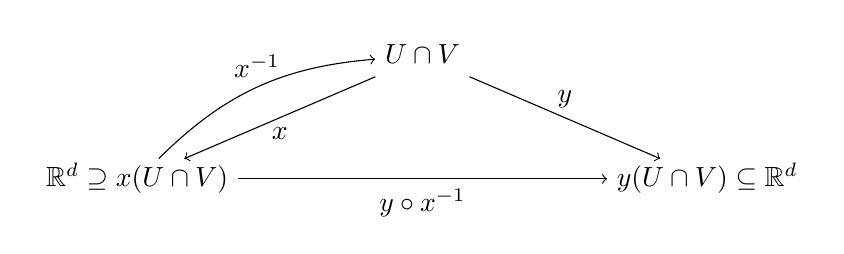
\begin{tikzpicture}
\matrix (m) [matrix of nodes, row sep=3em, column sep=5em, text height=1.5ex, text depth=0.25ex]
{  \text{ } & $U \cap V$ & \text{ } \\
$\mathbb{R}^d \supseteq x(U \cap V)$ & \text{ } & $y(U \cap V) \subseteq \mathbb{R}^d$ \\ };
\path[->]
(m-1-2) edge node[above] {$y$} (m-2-3)
        edge node[below] {$x$} (m-2-1);
\path[->]
(m-2-1) edge[bend left=20] node[above] {$x^{-1}$} (m-1-2)
        edge node[below] {$y \after x^{-1}$} (m-2-3);
\end{tikzpicture}
\]

The map $y \after x^{-1}$ is called the \textbf{chart transition map}, which maps an open set of $\mathbb{R}^d$ to another open set of $\mathbb{R}^d$. This map is continuous because it is composition of two continuous maps, Informally, these chart transition maps contain instructions on how to glue together the charts of an atlas,

\subsection{Manifold philosophy}
Often it is desirable (or indeed the only way) to define properties (e.g., `continuity') of real-world object (e.g., the curve $\gamma : \mathbb{R} \to M$) by judging suitable coordinates not on the `real-world' object itself, but on a chart-representation of that real world object.

For example, in the picture below, we can use the map $x \after \gamma$ to infer the continuity of the curve $\gamma$ in $U \subseteq M$.
\[
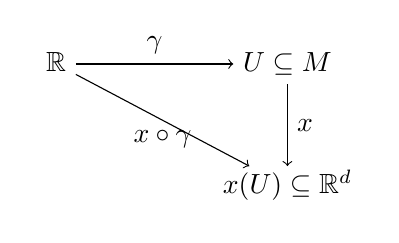
\begin{tikzpicture}
\matrix (m) [matrix of nodes, row sep=3em, column sep=5em, text height=1.5ex, text depth=0.25ex]
{  $\mathbb{R}$ & $U \subseteq M$ \\
\text{ } & $x(U) \subseteq \mathbb{R}^d$ \\ };
\path[->]
(m-1-1) edge node[above] {$\gamma$} (m-1-2)
        edge node[below] {$x \after \gamma$} (m-2-2);
\path[->]
(m-1-2) edge node[right] {$x$} (m-2-2);
\end{tikzpicture}
\]

However, we need to ensure that the defined property does not change if we change our chosen chart. For example, in the picture below, continuity in $x \after \gamma$ should imply $y \after \gamma$. This is true, since
$y \after \gamma = y \after (x^{-1} \after x) \after \gamma = (y \after x^{-1}) \after (x \after \gamma)$ is continuous because it is a composition of two continuous functions, thanks to the continuity of the chart transition map $y \after x^{-1}$.

\[
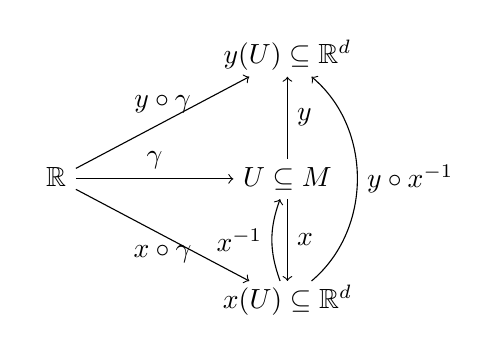
\begin{tikzpicture}
\matrix (m) [matrix of nodes, row sep=3em, column sep=5em, text height=1.5ex, text depth=0.25ex]
{  \text{ } & $y(U) \subseteq \mathbb{R}^d$ \\
$\mathbb{R}$ & $U \subseteq M$ \\
\text{ } & $x(U) \subseteq \mathbb{R}^d$ \\ };
\path[->]
(m-2-1) edge node[above] {$\gamma$} (m-2-2)
        edge node[above] {$y \after \gamma$} (m-1-2)
        edge node[below] {$x \after \gamma$} (m-3-2);
\path[->]
(m-2-2) edge node[right] {$y$} (m-1-2)
        edge node[right] {$x$} (m-3-2);
\path[->]
(m-3-2) edge[bend left=20] node[left] {$x^{-1}$} (m-2-2)
        edge[bend right=50] node[right] {$y \after x^{-1}$} (m-1-2);
\end{tikzpicture}
\]

What about differentiability? Does differentiability of $x \after \gamma$ guarantee differentiability of $y \after \gamma$? No. Since composition of a differentiable map and a continuous map might only be continuous, The solution is to restrict the atlas by removing those charts which are not differentiable. Thus, we have got rid of our problem. However, we must remember that with the present structure, we cannot define differentiability at manifold level since we do not know how to subtract or divide in $U \subseteq M$. Therefore, differentiability of $\gamma : \mathbb{R} \to M$ makes no sense yet. 
 % Manifolds
%\section*{Tutorial Topological manifolds}

filename: \verb|Sheet_1.2.pdf|

%\exercisehead{1}

\exercisehead{4: Before the invention of the wheel}

\emph{Another one-dimensional topological manifold. Another one?}

Consider set $F^1:= \lbrace (m,n)\in \mathbb{R}^2 | m^4 + n^4=1 \rbrace$, equipped with subset topology $\left. \mathcal{O}_{\text{std}} \right|_{F^1}$

\questionhead{$x:F^1 \to \mathbb{R}$ is what?}

\solutionhead{} EY : 20150525 The tutorial video \url{https://youtu.be/ghfEQ3u_B6g} is really good and this solution is how I'd write it, but it's really the same (I needed the practice).

\[
\boxed{ \begin{aligned}
   x : F^1 & \to \mathbb{R} \\ 
  (m,n) & \mapsto m
\end{aligned} }
\]

If $m=0$, $n^4=1$ so $n=\pm 1$ so it's not injective.  

Let the closed $n$-dim. upper half-space $\mathbb{H}^n \subseteq \mathbb{R}^1$.  Then
\[
\begin{aligned}
  \mathbb{H}^n = \lbrace (x_1 \dots x_n) \in \mathbb{R}^n | x_n \geq 0 \rbrace \\ 
  \text{int}\mathbb{H}^n = \lbrace (x_1 \dots x_n) \in \mathbb{R}^n | x_n > 0 \rbrace \\
  - \mathbb{H}^n = \lbrace (x_1 \dots x_n) \in \mathbb{R}^n | x_n \leq 0 \rbrace \\ 
  -\text{int}\mathbb{H}^n = \lbrace (x_1 \dots x_n) \in \mathbb{R}^n | x_n <0 \rbrace
\end{aligned}
\]

\questionhead{This map $x$ may be made injective by restricting its domain to either of 2 maximal open subsets of $F^1$. Which ones?}

\solutionhead{}

Let 
\[
\begin{aligned}
  & U_+ = F^1 \cap \text{int}\mathbb{H}^2 \\
  & U_- = F^1 \cap -\text{int}\mathbb{H}^2
\end{aligned}
\]

Look at 
\[
\begin{aligned}
  & x^4 = 1 - n^4 \\ 
  \Longrightarrow & x = \pm ( 1 - n^4)^{1/4}
\end{aligned}
\]

Then for 
\[
\begin{aligned}
  x_+^{-1}: (-1,1) \subseteq \mathbb{R} & \to U_+ \\ 
  m & \mapsto (m,(1-m^4)^{1/4}) \\
  x_-^{-1}: (-1,1) \subseteq \mathbb{R} & \to U_- \\ 
  m & \mapsto (m,-(1-m^4)^{1/4}) \\
\end{aligned}
\]
$x_+$,$x_-$ injective (since left inverse exists).  


\questionhead{Construct injective $y$}

\solutionhead{}

Let 
\[
\begin{aligned}
  & V_+ = F^1 \cap \text{int}\mathbb{H}^1 \\
  & V_- = F^1 \cap -\text{int}\mathbb{H}^1
\end{aligned}
\]

Then
\[
\begin{aligned}
  y_+:  V_+ & \to  (-1,1) \subseteq \mathbb{R} \\ 
  (m,n) & \mapsto n \\
  y_-: V_-  & \to  (-1,1) \subseteq \mathbb{R}  \\ 
  (m,n) & \mapsto n
\end{aligned}
\]

\questionhead{Construct inverse $y^{-1}$}
\solutionhead{}


For 
\[
\begin{aligned}
  y_+^{-1}: (-1,1) \subseteq \mathbb{R} & \to V_+ \\ 
  n & \mapsto ((1-n^4)^{1/4},n) \\
  y_-^{-1}: (-1,1) \subseteq \mathbb{R} & \to V_- \\ 
  n & \mapsto (-(1-n^4)^{1/4},n) \\
\end{aligned}
\]
$y_+$,$y_-$ injective (since left inverse exists).  



Note $\begin{aligned} & \quad \\ 
  & (-1,0) \notin U_+,U_- \\
  & (1,0) \notin U_+,U_- \\
\end{aligned}$

and 

 $\begin{aligned} & \quad \\ 
  & (0,1) \notin V_+,V_- \\
  & (0,-1) \notin V_+,V_- \\
\end{aligned}$


\questionhead{construct \emph{transition map } $x \circ y^{-1}$}

\solutionhead{}

\[
\begin{aligned}
& 
\begin{aligned}
   x_+y_+^{-1} : (0,1) \subseteq \mathbb{R} & \to (0,1) \subseteq \mathbb{R} \\ 
  n & \mapsto (1-n^4)^{1/4} 
\end{aligned}   \\ 
& 
\begin{aligned}
   x_-y_+^{-1} : (-1,0) \subseteq \mathbb{R} & \to (0,1) \subseteq \mathbb{R} \\ 
  n & \xrightarrow{ y_+^{-1} } ( (1-n^4)^{1/4}, n) \xrightarrow{ x_- } (1-n^4)^{1/4} 
\end{aligned}   \\ 
& \begin{aligned}
   x_+y_-^{-1} : (0,1) \subseteq \mathbb{R} & \to (-1,0) \subseteq \mathbb{R} \\ 
  n & \mapsto -(1-n^4)^{1/4} 
\end{aligned}   \\ 
& \begin{aligned}
   x_-y_-^{-1} : (-1,0) \subseteq \mathbb{R} & \to (-1,0) \subseteq \mathbb{R} \\ 
  n & \mapsto -(1-n^4)^{1/4} 
\end{aligned}   
\end{aligned}
\]

\questionhead{\dots Does the collection of these domains and maps form an atlas of $F^1$?}

Yes, with atlas

\[
\mathcal{A} = \lbrace \begin{aligned} & (U_+,x_+) \\
  & (U_-,x_-) \end{aligned}, \, \begin{aligned} & (V_+,y_+) \\ & (V_-,y_-) \end{aligned} \rbrace
\]

Clearly 
\[
\begin{gathered}
  U_+ \cup U_- \cup V_+ \cup V_- = (F^1 \cap \text{int}\mathbb{H}^2) \cup (F^1 \cap -\text{int}\mathbb{H}^2)\cup (F^1 \cap \text{int}\mathbb{H}^1) \cup (F^1 \cap -\text{int}\mathbb{H}^1) = \\
= F^1 \cap \mathbb{R}^2\backslash \lbrace (0,0) \rbrace = F^1
\end{gathered}
\]
and (the point is that) $x_{\pm},y_{\pm}$ are homeomorphisms of open sets of $F^1$ onto open sets of 1 dim. $\mathbb{R}^1$ (namely $(-1,1) \subseteq \mathbb{R}^1$), and so $\mathcal{A}$ is an atlas of $F^1$.  


\section{Multilinear Algebra}

\begin{framed}
\textbf{Motivation}: The essential object of study of linear algebra is vector space. However, a word of warning here. We will not equip space(time) with vector space structure. This is evident since, unlike in vector space, expressions such as $5 \cdot \text{Paris}$ and $\text{Paris} + \text{Vienna}$ do not make any sense. If multilinear algebra does not further our aim of studying spacetime, then why do we study it? The tangent spaces $T_pM$ (defined in Lecture 5) at a point $p$ of a smooth manifold $M$ (defined in Lecture 4) carries a vector space structure in a natural way even though the underlying position space(time) does not have a vector space structure. Once we have a notion of tangent space, we have a derived notion of a tensor. Tensors are very important in differential geometry. \\
It is beneficial to study vector spaces (and all that comes with it) abstractly for two reasons: (i) for construction of $T_pM$, one needs an intermediate vector space $C^{\infty}(M)$, and (ii) tensor techniques are most easily understood in an abstract setting.
\end{framed}

\subsection{Vector Spaces}
\begin{definition}
A $\mathbb{R}$-\textbf{vector space} is a triple $(V, +, \cdot)$, where
\begin{enumerate}[i)]
\item $V$ is a set,
\item $+ : V \times V \to V$ \quad (addition), and
\item $. : \mathbb{R} \times V \to V$ \quad (S-multiplication)
\end{enumerate}
satisfying the following:
\begin{enumerate}[a)]
\item $\forall u, v \in V : u + v = v + u$ \quad (commutativity of +)
\item $\forall u, v, w \in V : (u + v) + w = u + (v + w)$ \quad (associativity of +)
\item $\exists O \in V : \forall v \in V : O + v = v$ \quad (neutral element in +)
\item $\forall v \in V : \exists (-v) \in V : v + (-v) = 0$ \quad (inverse of element in +)

\item $\forall \lambda, \mu \in \mathbb{R}, \forall v \in V : \lambda \cdot (\mu \cdot v) = (\lambda \cdot \mu) \cdot v$ \quad (associativity in $\cdot$)
\item $\forall \lambda, \mu \in \mathbb{R}, \forall v \in V : (\lambda + \mu) \cdot v = \lambda \cdot v + \mu \cdot v$ \quad (distributivity of $\cdot$)
\item $\forall \lambda \in \mathbb{R}, \forall u, v \in V : \lambda \cdot u + \lambda \cdot v = \lambda \cdot (u + v)$ \quad (distributivity of $\cdot$)
\item $\exists 1 \in \mathbb{R} : \forall v \in V : 1 \cdot v = v$ \quad (unit element in $\cdot$)
\end{enumerate}
\end{definition}

\textbf{Terminology}: If $(V,+,\cdot)$ is a vector space, an element of $V$ is often referred to, informally, as a \textbf{vector}. But, we should remember that it makes no sense to call an element of $V$ a vector unless the vector space itself is specified.

\textbf{Example}: Consider a set of polynomials of fixed degree,
\begin{equation*}
P := \left\lbrace p:(-1,+1) \to \mathbb{R} \quad \Big| \quad p(x) = \displaystyle\sum_{n=0}^{N} p_n \cdot x^n, \text{ where } p_n \in \mathbb{R} \right\rbrace
\end{equation*} \\
with $\oplus : P \times P \to P$ with $(p,q) \mapsto p \oplus q : (p \oplus q)(x) = p(x) + q(x)$ and \\
$\odot : \mathbb{R} \times P \to P$ with $(\lambda,p) \mapsto \lambda \odot p : (\lambda \odot p)(x) = \lambda \cdot p(x)$. \textbf{$(P,\oplus,\odot)$} is a vector space.

\textbf{Caution}: \textit{We are considering real vector spaces, that is S-multiplication with the elements of $\mathbb{R}$. We shall often use same symbols `+' and `$\cdot$' for different vector spaces, but the context should make things clear. When $\mathbb{R}, \mathbb{R}^2$, etc. are used as vector spaces, the obvious (natural) operations shall be understood to be used.}

\subsection{Linear Maps}
These are the structure-respecting maps between vector spaces. 
\begin{definition}
If $(V,+_v,\cdot_v)$ and $(W,+_w,\cdot_w)$ are vector spaces, then $\phi : V \to W$ is called a \textbf{linear map} if
\begin{enumerate}[i)]
\item $\forall v, \tilde{v} \in V: \phi(v +_v \tilde{v}) = \phi(v) +_w \phi(\tilde{v})$, and
\item $\forall \lambda \in \mathbb{R}, v \in V : \phi(\lambda \cdot_v v) = \lambda \cdot_w \phi(v)$.
\end{enumerate}
\end{definition}

\textbf{Notation}: $\phi : V \to W \text{ is a linear map } \iff \phi : V \linearmapto W$

\textbf{Example}: Consider the vector space $(P,\oplus,\odot)$ from the above example, \\
Then, $\delta : P \to P$ with $p \mapsto \delta (p) := p^\prime$ is a linear map, because \\
$\forall p,q \in P : \delta(p \oplus q) = (p \oplus q)^\prime = p^\prime \oplus q^\prime = \delta(p) \oplus \delta(q)$ and \\
$\forall \lambda \in \mathbb{R}, p \in P : \delta(\lambda \odot p) = (\lambda \odot p)^\prime = \lambda \odot p^\prime$.

\begin{theorem}
If $\phi : U \linearmapto V$ and $\psi : V \linearmapto W$, then $\psi \after \phi : U \linearmapto W$.
\end{theorem}
\[
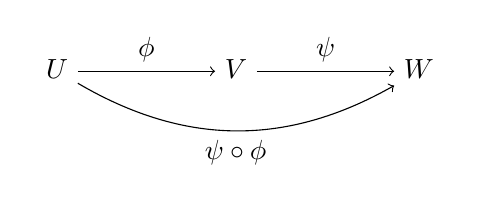
\begin{tikzpicture}
\matrix (m) [matrix of nodes, row sep=3em, column sep=5em, text height=1.5ex, text depth=0.25ex]
{  $U$ & $V$ & $W$ \\
};
\path[->]
(m-1-1) edge node[above] {$\phi$} (m-1-2)
        edge[bend right = 30] node[below] {$\psi \after \phi$} (m-1-3);
\path[->]
(m-1-2) edge node[above] {$\psi$} (m-1-3);
\end{tikzpicture}
\]

\begin{proof}
$ \forall u, \tilde{u} \in U, (\psi \after \phi)(u +_u \tilde{u}) = \psi(\phi(u +_u \tilde{u})) = \psi(\phi(u) +_v \phi(\tilde{u})) = \psi(\phi(u)) +_w \psi(\phi(\tilde{u})) = (\psi \after \phi)(u) +_w (\psi \after \phi)(\tilde{u}) $.

$ \forall \lambda \in \mathbb{R}, u \in U, (\psi \after \phi)(\lambda \cdot_u u) = \psi(\phi(\lambda \cdot_u u)) = \psi(\lambda \cdot_v \phi(u)) = \lambda \cdot_w \psi(\phi(u)) = \lambda \cdot_w (\psi \after \phi)(u) $
\end{proof}

\textbf{Example}: Consider the vector space $(P,\oplus,\odot)$ and the differential $\delta : P \to P$ with $p \mapsto \delta (p) := p^\prime$ from previous example. Then, $p^{\prime\prime}$, the second differential is also linear since it is composition of two linear maps, i.e., $\delta \after \delta : P \linearmapto P$.

\subsection{Vector Space of Homomorphisms}
\begin{definition}
If $(V, +, \cdot)$ and $(W, +, \cdot)$ are vector spaces, then $Hom(V,W) := \left\lbrace \phi : V \linearmapto W \right\rbrace$.
\end{definition}

\begin{theorem}
$(Hom(V,W),+,\cdot)$ is a vector space with \\
$+ : Hom(V,W) \times Hom(V,W) \to Hom(V,W)$ with $(\phi,\psi) \mapsto \phi + \psi : (\phi + \psi)(v) = \phi(v) + \psi(v)$ and \\
$\cdot : \mathbb{R} \times Hom(V,W) \to Hom(V,W)$ with $(\lambda,\phi) \mapsto \lambda \cdot \phi : (\lambda \cdot \phi)(v) = \lambda \cdot \phi(v)$.
\end{theorem}

\textbf{Example}: $(Hom(P,P),+,\cdot)$ is a vector space. $\delta \in Hom(P,P)$, $\delta \after \delta \in Hom(P,P)$, $\delta \after \delta \after \delta \in Hom(P,P)$, etc. Therefore, maps such as $5 \cdot \delta + \delta \after \delta \in Hom(P,P)$. Thus, mixed order derivatives are in $Hom(P,P)$, and hence linear.

\subsection{Dual Vector Spaces}
\begin{definition}
If $(V, +, \cdot)$ is a vector space, and $V^{\ast} := \left\lbrace \phi : V \linearmapto \mathbb{R} \right\rbrace = Hom(V,\mathbb{R})$ then \\
$(V^{\ast},+,\cdot)$ is called the \textbf{dual vector space to V}.
\end{definition}

\textbf{Terminology}: $\omega \in V^{\ast}$ is called, informally, a \textbf{covector}.

\textbf{Example}: Consider $I : P \linearmapto \mathbb{R}$, i.e., $I \in P^\ast$. We define $I(p) := \int_0^1 \! p(x) \, \mathrm{d}x$, which can be easily checked to be linear with $I(p + q) = I(p) + I(q)$ and $I(\lambda \cdot p) = \lambda \cdot I(p)$. Thus $I$ is a covector, which is the integration operator $\int_0^1 \! ( \quad ) \, \mathrm{d}x$ which eats a function. 

\textit{Remarks: We shall also see later that the gradient is a covector. In fact, lots of things in physicist's life, which are covectors, have been called vectors not to bother you with details. But covectors are neither esoteric nor unnatural.}

\subsection{Tensors}
We can think of tensors as multilinear maps.

\begin{definition}
Let $(V, +, \cdot)$ be a vector space. An \textbf{(r,s) -tensor} T over V is a multilinear map
\begin{equation*}
T : \underbrace{V^\ast \times V^\ast \times \dots \times V^\ast}_\text{r times} \times \underbrace{V \times V \times \dots \times V}_\text{s times} \linearmapto \mathbb{R}
\end{equation*}
\end{definition}

\textbf{Example}: If T is a (1,1)-tensor, then \\
$T(\omega_1 + \omega_2, v) = T(\omega_1, v) + T(\omega_2, v)$, \\
$T(\omega, v_1 + v_2) = T(\omega, v_1) + T(\omega, v_2)$, \\
$T(\lambda \cdot \omega, v) = \lambda \cdot T(\omega, v)$, and \\
$T(\omega, \lambda \cdot v) = \lambda \cdot T(\omega, v)$. \\
Thus, $T(\omega_1 + \omega_2, v_1 + v_2) = T(\omega_1, v_1) + T(\omega_1, v_2) + T(\omega_2, v_1) + T(\omega_2, v_2)$. \\

\textit{Remarks}: Sometimes it is said that a (1,1)-tensor is something that eats a vector and outputs a vector. Here is why. For $T : V^\ast \times V \linearmapto \mathbb{R}$, define $\phi_T : V \linearmapto (V^\ast)^\ast$ with $v \mapsto T(( \cdot ), v)$. But, clearly $T(( \cdot ), v) : V^\ast \linearmapto \mathbb{R}$, which eats a covector and spits a number. In other words, $T(( \cdot ), v) \in (V^\ast)^\ast$. Although we are yet to define dimension, let us just trust, for the time being, that for finite-dimensional vector spaces, $(V^\ast)^\ast = V$. So, $\phi_T : V \linearmapto V$.

\textbf{Example}: Let $g : P \times P \linearmapto \mathbb{R}$ with $(p,q) \mapsto \int_{-1}^1 \! p(x) \cdot q(x) \, \mathrm{d}x$. Then, $g$ is a (0,2)-tensor over $P$.

\subsection{Vectors and Covectors as Tensors}
\begin{theorem}
If $(V,+,\cdot)$ is a vector space, $\omega \in V^\ast$ is a (0,1)-tensor.
\end{theorem}
\begin{proof}
$\omega \in V^\ast$ and, by definition, $V^{\ast} := \left\lbrace \phi : V \linearmapto \mathbb{R} \right\rbrace$, which is a collection of (0,1)-tensors. 
\end{proof}

\begin{theorem}
If $(V,+,\cdot)$ is a vector space, $v \in V$ is a (1,0)-tensor.
\end{theorem}
\begin{proof}
We have already stated, without proof and without defining dimensions, that $V = (V^\ast)^\ast$ for finite-dimensional vector spaces. Therefore, $v \in V \implies v \in (V^\ast)^\ast \implies v \in \left\lbrace \phi : V^\ast \linearmapto \mathbb{R} \right\rbrace \implies$ $v$ is a (1,0)-tensor.
\end{proof}

\subsection{Bases}
\begin{definition}
Let $(V,+,\cdot)$ is a vector space. A subset $B \subseteq V$ is called a \textbf{basis} if \\
$\forall v \in V, \exists ! finite v_1,v_2,\dotsc,v_n \in B, \exists ! f_1,f_2,\dotsc,f_n \in \mathbb{R} : v = \displaystyle\sum_{i=1}^n f_i \cdot v_i$. 
\end{definition}

\begin{definition}
A vector space $(V,+,\cdot)$ with a basis $B$ is said to be \textbf{$d$-dimensional} if $B$ has $d$ elements. In other words, $dim V := d$.
\end{definition}

\textit{Remarks: The above definition is well-defined only if every basis of a vector space has the same number of elements.}

\textbf{Remarks}: Let $(V,+,\cdot)$ is a vector space. Having chosen a basis $e_1,e_2,\dotsc,e_n$, we may uniquely associate $v \mapsto (v_1,v_2,\dotsc,v_n)$, these numbers being the components of $v$ w.r.t. chosen basis where $v = \displaystyle\sum_{i=1}^n v_i \cdot e_i$.

\subsection{Basis for the Dual Space}
Let $(V,+,\cdot)$ is a vector space. Having chosen a basis $e_1,e_2,\dotsc,e_n$ for $V$, we can choose a basis $\epsilon^1,\epsilon^2,\dotsc,\epsilon^n$ for $V^\ast$ entirely independent of basis of $V$. However, it is more economical to require that
\begin{equation*}
\epsilon^a (e_b) = \delta_b^a = \begin{cases}
1 &\quad \text{if } a = b \\
0 &\quad \text{if } a \neq b \\
\end{cases}
\end{equation*} This uniquely determines $\epsilon^1,\epsilon^2,\dotsc,\epsilon^n$ from choice of $e_1,e_2,\dotsc,e_n$.

\textit{Remarks: The reason for using indices as superscripts or subscripts is to be able to use the Einstein summation convention, which will be helpful in dropping cumbersome $\sum$ symbols in several equations.}

\begin{definition}
For a basis $e_1,e_2,\dotsc,e_n$ of vector space $(V,+,\cdot)$, $\epsilon^1,\epsilon^2,\dotsc,\epsilon^n$ is called the \textbf{dual basis} of the dual space, if $\epsilon^a (e_b) = \delta_b^a$.
\end{definition}

\textbf{Example}: Consider polynomials $P$ of degree 3. Choose $e_0,e_1,e_2,e_3 \in P$ such that $e_0(x) = 1, e_1(x) = x, e_2(x) = x^2 and e_3(x) = x^3$. Then, it can be easily verified that the dual basis is $\epsilon^a = \displaystyle\frac{1}{a!}\partial^a\Big|_{x=0}$.

\subsection{Components of Tensors}
\label{ss:L3_TensorComponents}
\begin{definition}
Let $T$ be a $(r,s)$-tensor over a $d$-dimensional (finite) vector space $(V,+,\cdot)$. Then, with respect to some basis $\lbrace e_1, \dotsc, e_r \rbrace$ and the dual basis $\lbrace \epsilon^1, \dotsc, \epsilon^s \rbrace$, define $(r+s)^d$ real numbers
\begin{equation*}
T\indices{^{i_1 \dots i_r}_{j_1 \dots j_s}} := T(\epsilon^{i_1}, \dotsc, \epsilon^{i_r}, e_{j_1}, \dotsc, e_{j_s})
\end{equation*} such that the indices $i_1, \dotsc, i_r, j_1, \dotsc, j_s$ take all possible values in the set $\lbrace 1,\dotsc,d \rbrace$. These numbers $T\indices{^{i_1 \dots i_r}_{j_1 \dots j_s}}$ are called the \textbf{components of the tensor} $T$ w.r.t. the chosen basis.
\end{definition}

This is useful because knowing components (and the basis w.r.t which these components have been chosen), one can reconstruct the entire tensor.

\textbf{Example}: If $T$ is a $(1,1)$-tensor, then $T\indices{^{i}_{j}} := T(\epsilon^i,e_j)$. Then\\
\begin{equation*}
T(\omega,v) = T\left(\sum_{i=1}^d \omega_i \cdot \epsilon^i,\sum_{j=1}^d v^j \cdot e_j \right) = \sum_{i=1}^d \sum_{j=1}^d \omega_i v^j T(\epsilon^i,e_j) = \sum_{i=1}^d \sum_{j=1}^d \omega_i v^j T\indices{^{i}_{j}} =: \omega_i v^j T\indices{^{i}_{j}}
\end{equation*}
 % Multilinear Algebra

\section{Differential Manifolds}
\begin{framed}
\textbf{Motivation}: So far we have dealt with topological manifolds which allow us to talk about continuity. But to talk about smoothness of curves on manifolds, or velocities along these curves, we need something like differentiability. Does the structure of topological manifold allow us to talk about differentiability? The answer is a resounding no.

So this lecture is about figuring out what structure we need to add on a topological manifold $M$ to start talking about differentiability of curves ($\mathbb{R} \to M$) on a manifold, or differentiability of functions ($M \to \mathbb{R}$) on a manifold, or differentiability of maps ($M \to N$) from one manifold $M$ to another manifold $N$. 
\end{framed}

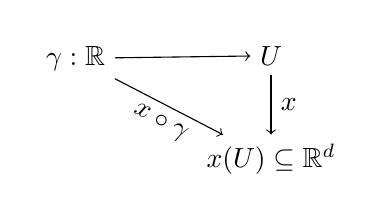
\begin{tikzpicture}[decoration=snake]
  \matrix (m) [matrix of math nodes, row sep=2em, column sep=3em, minimum width=1em]
  {
\gamma : \mathbb{R} & U \\
& x(U) \subseteq \mathbb{R}^d \\ 
};
  \path[->]
  (m-1-1) edge node [above] {$$} (m-1-2)
          edge node [sloped, anchor=center, below] {$x \circ \gamma$} (m-2-2)
  (m-1-2) edge node [right] {$x$} (m-2-2);
\end{tikzpicture}

\underline{idea}. try to ``lift'' the undergraduate notion of differentiability of a curve on $\mathbb{R}^d$ to a notion of differentiability of a curve on $M$

\underline{Problem} Can this be well-defined under change of chart?

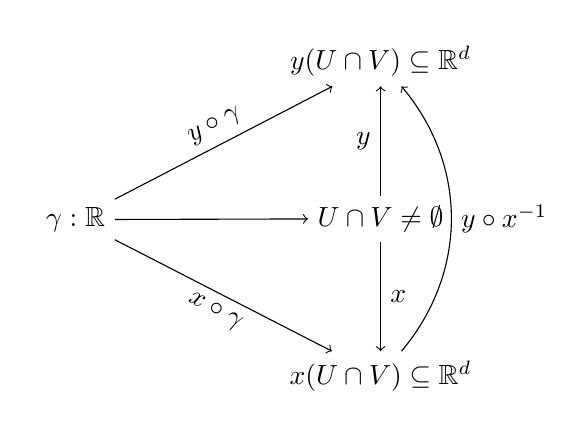
\begin{tikzpicture}[decoration=snake]
  \matrix (m) [matrix of math nodes, row sep=4em, column sep=6em, minimum width=2em]
  {
    & y(U\cap V) \subseteq \mathbb{R}^d \\ 
\gamma : \mathbb{R} & U \cap V \neq \emptyset \\
& x(U\cap V) \subseteq \mathbb{R}^d \\ 
};
  \path[->]
  
  (m-2-1) edge node [auto] {$$} (m-2-2)
          edge node [sloped, anchor=center, below] {$x \circ \gamma$} (m-3-2)
          edge node [sloped, anchor=center, above] {$y \circ \gamma$} (m-1-2)
  (m-2-2) edge node [auto] {$x$} (m-3-2)
          edge node [auto] {$y$} (m-1-2)
  (m-3-2) edge [bend right=40] node [right] {$y\circ x^{-1}$} (m-1-2);
\end{tikzpicture}

$x\circ \gamma$ undergraduate differentiable (``as a map $\mathbb{R} \to \mathbb{R}^d$'')

\[
\begin{gathered}
  \underbrace{y\circ \gamma}_{\text{maybe only continuous, but not undergraduate differentiable} } =  \underbrace{ ( \overbrace{ y\circ x^{-1}}^{\mathbb{R}^d \to \mathbb{R}^d }   )}_{\text{continuous}}  \circ \underbrace{ \overbrace{ (x\circ \gamma) }^{\mathbb{R}\to \mathbb{R}^d} }_{ \text{ undergrad differentiable } }  = y \circ (x^{-1} \circ x) \circ \gamma
\end{gathered}
\]

At first sight, strategy does not work out.  

\subsection{Compatible charts}

In section 1, we used any imaginable charts on the top. mfd. $(M,\mathcal{O})$.  

To emphasize this, we may say that we took $U$ and $V$ from the \emph{maximal atlas} $\mathcal{A}$ of $(M,\mathcal{O})$.  


\begin{definition}
Two charts $(U,x)$ and $(V,y)$ of a top. mfd. are called \ding{96}-compatible if 
either
\begin{enumerate}
  \item[(a)] $U \cap V = \emptyset$
or  \item[(b)] $U\cap V \neq \emptyset$
\end{enumerate}
chart transition maps have undergraduate \ding{96} property.

EY : 20151109 e.g. since $\mathbb{R}^d \to \mathbb{R}^d$, can use undergradate \ding{96} property such as continuity or differentiability.

\[
\begin{aligned}
  & y \circ x^{-1} : x(U \cap V) \subseteq \mathbb{R}^d  \to y(U\cap V) \subseteq \mathbb{R}^d  \\
  & x\circ y^{-1} : y(U\cap V) \subseteq \mathbb{R}^d   \to x(U\cap V) \subseteq \mathbb{R}^d
\end{aligned}
\]
\end{definition}

\underline{Philosophy}: 

\begin{definition}
  An atlas $\mathcal{A}_{\text{\ding{96}}}$ is a \ding{96}-compatible atlas if any two charts in $\mathcal{A}_{\text{\ding{96}}}$ are \ding{96}-compatible.

\end{definition}

\begin{definition}
  A \textbf{\ding{96}-manifold} is a triple $(\underbrace{ M,\mathcal{O} }_{\text{top. mfd.} }, \mathcal{A}_{\text{\ding{96}}})$ \quad \, $\mathcal{A}_{\text{\ding{96}}} \subseteq \mathcal{A}_{\text{maximal}} $
\end{definition}


\begin{tabular}{ l | c  l}
\ding{96} &  undergraduate  \ding{96} &  \\
\hline
$C^0$ & $C^0(\mathbb{R}^d \to \mathbb{R}^d) =$  &  continuous maps w.r.t. $\mathcal{O}$  \\
$C^1$ & $C^1(\mathbb{R}^d \to \mathbb{R}^d) = $  &  differentiable (once) and is continuous  \\
$C^k$ & & $k$-times continuously differentiable \\
$D^k$ & & $k$-times differentiable \\
$\vdots$ & & \\
$C^{\infty}$ & $C^{\infty}(\mathbb{R}^d \to \mathbb{R}^d)$ & \\
$\mathbin{\rotatebox[origin=c]{-90}{$\supseteq$}}$ & &  \\
$C^{\omega}$ & $\exists $  multi-dim. Taylor exp.  &  \\
$\mathbb{C}^{\infty}$ & satisfy Cauchy-Riemann equations, pair-wise & 
\end{tabular}


EY : 20151109 Schuller says: $C^k$ is easy to work with because you can judge $k$-times cont. differentiability from existence of all partial derivatives \textbf{and} their continuity.  There are examples of maps that partial derivatives exist but are not $D^k$, $k$-times differentiable.  

\begin{theorem}[Whitney]
%  Any $C^{k\geq 1}$-manifold $(M,\mathcal{O}, \mathcal{A}_{C^{k\geq 1}})$  
  Any $C^{k\geq 1}$-atlas, $\mathcal{A}_{C^{k\geq 1}}$ of a topological manifold \emph{contains} a $C^{\infty}$-atlas.  

Thus we may w.l.o.g. always consider $C^{\infty}$-manifolds, ``smooth manifolds'', unless we wish to define Taylor expandibility/complex differentiability \dots
\end{theorem}

EY : 20151109 Hassler Whitney \footnote{\url{http://mathoverflow.net/questions/8789/can-every-manifold-be-given-an-analytic-structure}}

\begin{definition}
  A smooth manifold $(\underbrace{ M,\mathcal{O} }_{\text{top. mfd. } }, \underbrace{ \mathcal{A}}_{C^{\infty}-\text{atlas}} )$ 
\end{definition}

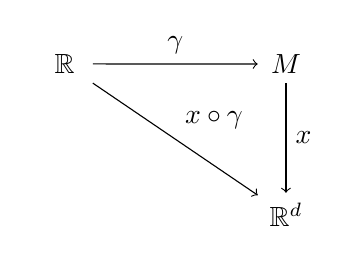
\begin{tikzpicture}
  \matrix (m) [matrix of math nodes, row sep=4em, column sep=6em, minimum width=2em]
  {
 \mathbb{R} & M   \\
&  \mathbb{R}^d \\ 
};
  \path[->]  
  (m-1-1) edge node [auto] {$\gamma$} (m-1-2)
          edge node [auto] {$x\circ \gamma$} (m-2-2)
  (m-1-2) edge node [auto] {$x$} (m-2-2);
\end{tikzpicture}
EY: 20151109 Schuller was explaining that the trajectory is real in $M$; the coordinate maps to obtain coordinates is $x\circ \gamma$

\subsection{Diffeomorphisms}

$M \xrightarrow{ \phi } N$

If $M,N$ are naked sets, the structure preserving maps are the bijections (invertible maps).  

e.g. $\lbrace 1,2,3 \rbrace \to \lbrace a,b \rbrace$

\begin{definition}
  $M \cong_{\text{set}} N$ (set-theoretically) isomorphic if $\exists \, $ bijection $\phi : M \to N$
\end{definition}

\underline{Examples}.  $\mathbb{N} \cong_{\text{set}} \mathbb{Z}$ \\
$\mathbb{N} \cong_{\text{set}} \mathbb{Q}$  (EY: 20151109 Schuller says from diagonal counting)\\
$\mathbb{N} \cancel{\cong_{\text{set}}} \mathbb{R}$

Now $(M, \mathcal{O}_M) \cong_{\text{top}} (N,\mathcal{O}_N)$ (topl.) isomorphic $=$ ``homeomorphic'' $\exists \, $ bijection $\phi : M \to N$  \\
\phantom{ \quad \quad \, } $\phi, \phi^{-1}$ are continuous.  

$(V,+,\cdot) \cong_{\text{vec}} ( W,+_w,\cdot_w)$ (EY: 20151109 vector space isomorphism) if \\
$\exists \, \text{ bijection } \phi : V \to W$ linearly

\underline{finally}

\begin{definition}
  Two $C^{\infty}$-manifolds \\
  $(M,\mathcal{O}_M, \mathcal{A}_M)$ and $(N,\mathcal{O}_N, \mathcal{A}_N)$ are said to be \textbf{diffeomorphic} if $\exists \, $ bijection $\phi : M \to N$ s.t. 
\[
\begin{aligned} & \phi : M \to N \\
  & \phi^{-1} : N \to M \end{aligned}
    \]
are both $C^{\infty}$-maps

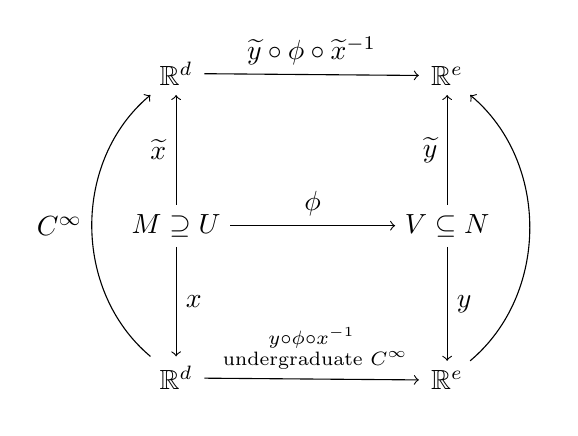
\begin{tikzpicture}
  \matrix (m) [matrix of math nodes, row sep=4em, column sep=6em, minimum width=2em]
  {
 \mathbb{R}^d & \mathbb{R}^e   \\
M \supseteq U &  V\subseteq N   \\ 
\mathbb{R}^d & \mathbb{R}^e \\
};
  \path[->]  
  (m-1-1) edge node [auto] {$\widetilde{y} \circ \phi \circ \widetilde{x}^{-1}$} (m-1-2)
  (m-2-1) edge node [auto] {$\widetilde{x}$} (m-1-1)
          edge node [auto] {$\phi$} (m-2-2)
          edge node [auto] {$x$} (m-3-1)
  (m-3-1) edge node [auto] {$ \substack{ y\circ \phi \circ x^{-1} \\ 
 \text{ undergraduate } C^{\infty} }$} (m-3-2)
          edge [bend left=50] node [auto] {$C^{\infty}$} (m-1-1)
  (m-2-2) edge node [auto] {$\widetilde{y}$} (m-1-2) 
          edge node [auto] {$y$} (m-3-2)
  (m-3-2) edge [bend right=50] node [auto] {$$} (m-1-2);
\end{tikzpicture}


\end{definition}

\begin{theorem}
  $\# = $ number of $C^{\infty}$-manifolds one can make out of a given $C^0$-manifolds (if any) - up to diffeomorphisms.  

\begin{tabular}{l | c r }
  $\text{dim}M$ &  $\#$ &  \\
  \hline
  1  & 1  & Morse-Radon theorems \\
 2  & 1  & Morse-Radon theorems \\
 3 & 1  & Morse-Radon theorems \\
4 & uncountably infinitely many & \\
5 &   finite  & surgery theory \\
6 &  finite & surgery theory \\
\vdots & finite & surgery theory
\end{tabular}

\end{theorem}

EY : 20151109 cf. \url{http://math.stackexchange.com/questions/833766/closed-4-manifolds-with-uncountably-many-differentiable-structures}  \\
\href{http://www.maths.ed.ac.uk/~aar/papers/scorpan.pdf}{The wild world of 4-manifolds}
 % Differentiable Manifolds
%\section*{Tutorial 4 Differentiable Manifolds}

EY : 20151109 The \url{gravity-and-light.org} website, where you can download the tutorial sheets \emph{and} the full length videos for the tutorials and lectures, are no longer there.  $=($  

Hopefully, the YouTube video will remain: \url{https://youtu.be/FXPdKxOq1KA?list=PLFeEvEPtX_0RQ1ys-7VIsKlBWz7RX-FaL}

\exercisehead{1: True or false?} \emph{These basic questions are designed to spark discussion and as a self-test.}

Tick the correct statements, but not the incorrect ones!

\begin{enumerate}
  \item[(a)] The function $f: \mathbb{R} \to \mathbb{R}$, \dots
    \begin{itemize}
      \item  
      \item
      \item \dots , defined by $f(x) = |x^3|$, lies in $C^3(\mathbb{R} \to \mathbb{R})$.  

\solutionhead{1a3} For $f: \mathbb{R} \to \mathbb{R}$, $f(x) = |x^3| = \begin{cases} x^3 & \text{ if } x \geq 0 \\
  -x^3 & \text{ if } x < 0 \end{cases}$ 
\[
\begin{aligned}
  & f'(x) = \begin{cases} 3x^2  & \text{ if } x \geq 0 \\
    -3x^2 & \text{ if } x < 0 \end{cases} \\ 
  & f''(x) = \begin{cases} 6x  & \text{ if } x \geq 0 \\
    -6x & \text{ if } x < 0 \end{cases} 
\end{aligned}
\]
Thus, 
\[
\boxed{ f(x) = |x^3| \in C^1(\mathbb{R}) \text{ but } f(x) \notin C^2(\mathbb{R}) \subseteq C^3(\mathbb{R}) }
\]
      \item
      \item
\end{itemize}
  \item[(b)]
  \item[(c)]
\end{enumerate}

\textbf{Short} \exercisehead{4: Undergraduate multi-dimensional analysis }

\emph{A good notation and basic results for partial differentiation}.

For a map $f: \mathbb{R}^d \to \mathbb{R}$ we denote by the map $\partial_i f: \mathbb{R}^d \to \mathbb{R}$ the partial derivative with respect to the $i$-th entry.

\questionhead{:} Given a function
\[
f: \mathbb{R}^3 \to \mathbb{R}; \, (\alpha, \beta, \delta) \mapsto f(\alpha,\beta,\delta) := \alpha^3\beta^2 + \beta^2 \delta + \delta
\]
calculate the values of the following derivatives:

\solutionhead{:}

\begin{itemize}
  \item $(\partial_2f)(x,y,z) = $
  \item $(\partial_1f)(\square,\circ,*) =$
  \item $(\partial_1 \partial_2 f)(a,b,c) = $ 
  \item $(\partial_3^2 f)(299,1222,0) =$
\end{itemize}

EY: 20151110

For $f(\alpha,\beta,\delta) := \alpha^3\beta^2 + \beta^2 \delta + \delta$, or $f(x,y,z) = x^3 y^2 + y^2 z + z$, 
\[
\begin{aligned}
  & (\partial_2 f) = 2(x^3y+yz) \\ 
  & (\partial_1 f) = 3x^2 y^2 \\ 
  & (\partial_1\partial_2 f) = 6x^2 y \\ 
  & (\partial_3^2f) = 0 
\end{aligned}
\]
and so 
\begin{itemize}
  \item $(\partial_2f)(x,y,z) = 2(x^3 y + yz)  $
  \item $(\partial_1f)(\square,\circ,*) = 3\square^2 \circ^2$
  \item $(\partial_1 \partial_2 f)(a,b,c) = 6a^2 b$ 
  \item $(\partial_3^2 f)(299,1222,0) = 0$
\end{itemize}



\exercisehead{5: Differentiability on a manifold}

\emph{How to deal with functions and curves in a chart} 

Let $(M, \mathcal{O}, \mathcal{A})$ be a smooth $d$-dimensional manifold.  Consider a chart $(U,x)$ of the atlas $\mathcal{A}$ together with a smooth curve $\gamma : \mathbb{R} \to U$ and a smooth function $f:U \to \mathbb{R}$ on the domain $U$ of the chart. 

\questionhead{:} Draw a commutative diagram containing the chart domain, chart map, function, curveand the respective representatives of the function and the curve in the chart. 

\solutionhead{:}

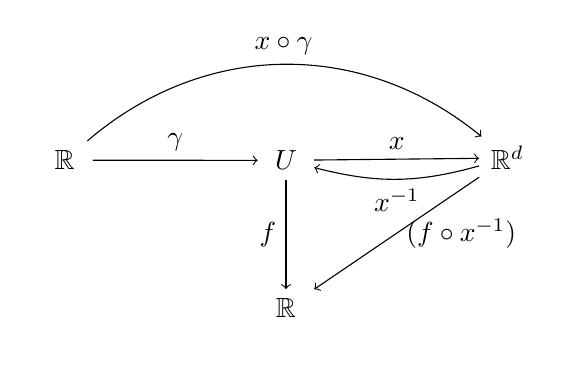
\begin{tikzpicture}[decoration=snake]
  \matrix (m) [matrix of math nodes, row sep=4em, column sep=6em, minimum width=2em]
  {
 \mathbb{R} & U & \mathbb{R}^d \\
& \mathbb{R} &  \\
};
  \path[->]
  (m-1-1) edge node [above] {$\gamma$} (m-1-2)
          edge [bend left=40] node [auto] {$x\circ \gamma$} (m-1-3)
  (m-1-3) edge [bend left=15] node [auto] {$x^{-1}$} (m-1-2)
          edge node [right] {$(f\circ x^{-1})$ } (m-2-2)
  (m-1-2) edge node [left] {$f$} (m-2-2)
          edge node [auto] {$x$} (m-1-3);
\end{tikzpicture} \quad \quad \, 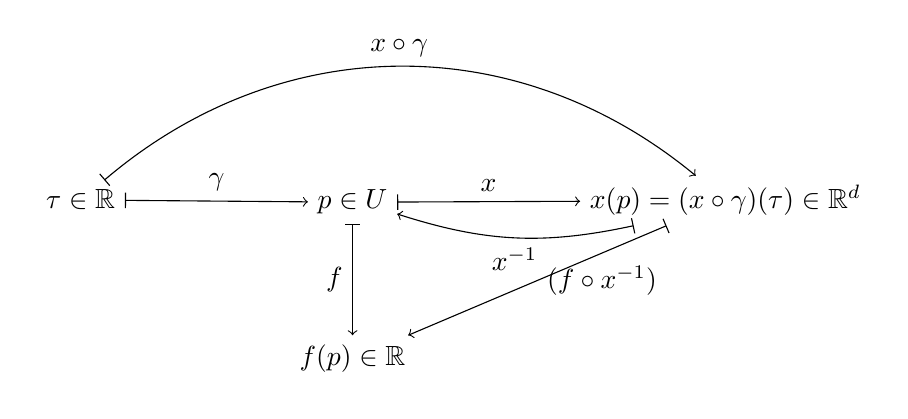
\begin{tikzpicture}[decoration=snake]
  \matrix (m) [matrix of math nodes, row sep=4em, column sep=6em, minimum width=2em]
  {
 \tau \in \mathbb{R} & p \in U & x(p) = (x\circ \gamma)(\tau) \in \mathbb{R}^d \\
& f(p) \in \mathbb{R} &  \\
};
  \path[|->]
  (m-1-1) edge node [above] {$\gamma$} (m-1-2)
          edge [bend left=40] node [auto] {$x\circ \gamma$} (m-1-3)
  (m-1-3) edge [bend left=15] node [auto] {$x^{-1}$} (m-1-2)
          edge node [right] {$(f\circ x^{-1})$ } (m-2-2)
  (m-1-2) edge node [left] {$f$} (m-2-2)
          edge node [auto] {$x$} (m-1-3);
\end{tikzpicture}



\questionhead{:} Consider, for $d=2$,
\[
(x\circ \gamma)(\lambda):= (\cos{(\lambda)}, \sin{(\lambda)} ) \text{ and } (f\circ x^{-1})((x,y)) := x^2 +y^2
\]
Using the chain rule, calculate
\[
(f\circ \gamma)'(\lambda)
\]
explicitly.

\solutionhead{:}

EY : 20151109 Indeed, the domains and codomains of this $f\gamma$ mapping makes sense, from $\mathbb{R} \to \mathbb{R}$ for 
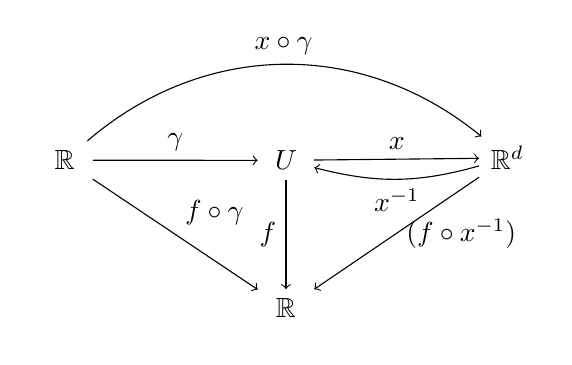
\begin{tikzpicture}[decoration=snake]
  \matrix (m) [matrix of math nodes, row sep=4em, column sep=6em, minimum width=2em]
  {
 \mathbb{R} & U & \mathbb{R}^d \\
& \mathbb{R} &  \\
};
  \path[->]
  (m-1-1) edge node [above] {$\gamma$} (m-1-2)
          edge [bend left=40] node [auto] {$x\circ \gamma$} (m-1-3)
          edge node [auto] {$f\circ \gamma$} (m-2-2)
  (m-1-3) edge [bend left=15] node [auto] {$x^{-1}$} (m-1-2)
          edge node [right] {$(f\circ x^{-1})$ } (m-2-2)
  (m-1-2) edge node [left] {$f$} (m-2-2)
          edge node [auto] {$x$} (m-1-3);
\end{tikzpicture} \quad \quad \, 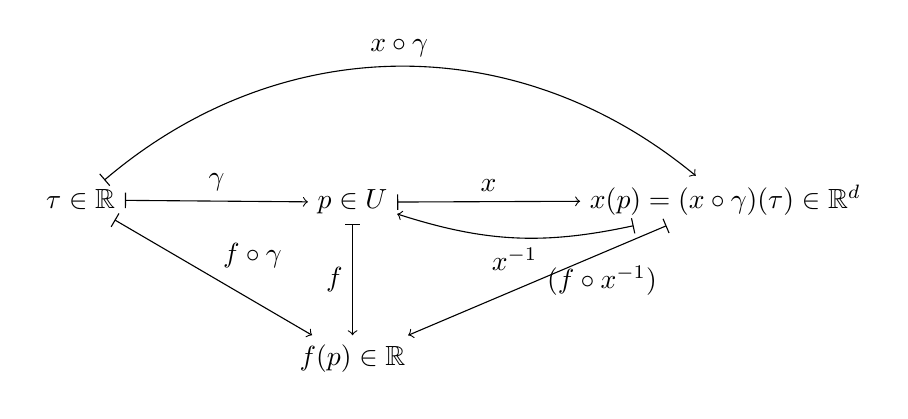
\begin{tikzpicture}[decoration=snake]
  \matrix (m) [matrix of math nodes, row sep=4em, column sep=6em, minimum width=2em]
  {
 \tau \in \mathbb{R} & p \in U & x(p) = (x\circ \gamma)(\tau) \in \mathbb{R}^d \\
& f(p) \in \mathbb{R} &  \\
};
  \path[|->]
  (m-1-1) edge node [above] {$\gamma$} (m-1-2)
          edge [bend left=40] node [auto] {$x\circ \gamma$} (m-1-3)
          edge node [auto] {$f\circ \gamma$} (m-2-2)
  (m-1-3) edge [bend left=15] node [auto] {$x^{-1}$} (m-1-2)
          edge node [right] {$(f\circ x^{-1})$ } (m-2-2)
  (m-1-2) edge node [left] {$f$} (m-2-2)
          edge node [auto] {$x$} (m-1-3);
\end{tikzpicture}

\[
\begin{gathered}
  (f\circ \gamma)'(\lambda) = (Df)\cdot \dot{\gamma}(\lambda) = \frac{ \partial f}{ \partial x^j} \dot{\gamma}^j(\lambda) = 2x (-\sin{\lambda} ) + 2y \cos{\lambda} = 2(-\cos{\lambda} \sin{\lambda} + \sin{\lambda} \cos{\lambda} ) = 0 
\end{gathered}
\]


\section{Tangent Spaces}
Lead question: ``What is the velocity of a curve $\gamma : \R \to M$ at the point $p$ of the curve in $M$?''

\subsection{Velocities}
% \url{https://youtu.be/pepU_7NJSGM?t=1m30s}
\begin{definition} Let $\mfd$ be a smooth manifold. Let there be a curve $\gamma : \R \to M$, which is at least $C^1$. Suppose $\gamma(\lambda_0) =p$. The \textbf{velocity} of $\gamma$ at the point $p$ of the curve $\gamma$ is the linear map \\
\begin{equation}\label{eq_velocity}
v_{\gamma, p} : C^{\infty}(M) \linearmapto \R \text{ with }
f \mapsto v_{\gamma,p}(f):= (f \after \gamma)^{\prime}(\lambda_0)
\end{equation}
where $C^{\infty}(M) := \lbrace f: M \to \R \, | \, f \text{ is a smooth function } \rbrace$ equipped with \\
$(f \oplus g)(p) := f(p) + g(p)$ and $(\lambda \otimes g)(p) := \lambda \cdot g(p)$ is a vector space.
\end{definition}

\begin{SCfigure}[5][h]
\label{fig:L5_fAfterGamma}
  \centering
	\begin{tikzpicture}
	  \matrix (m) [matrix of math nodes, row sep=4em, column sep=6em, minimum width=2em]
	  {
		\R & M & \R \\
	  };
	  \path[->]  
	  (m-1-1) edge node [auto] {$\gamma$} (m-1-2)
	          edge [bend right=30] node [auto] {$f \after \gamma$} (m-1-3)
	  (m-1-2) edge node [auto] {$f $} (m-1-3);
	\end{tikzpicture}
    \caption{$f \after \gamma$. Intuition: If the first $\R$ is thought of as time, and $f$ as temperature, then $f \after \gamma$ relates time and temperature and $(f \after \gamma)^\prime$ is the rate of change of temperature as you run around the curve.}
\end{SCfigure}

\underline{past}: `` $\underbrace{v^i}_{\text{vector in past}} (\partial_i f) = (\underbrace{v^i \partial_i}_{\text{vector as map}})f$ \\
\textit{In an imprecise way, we could say that we want vectors to survive as the directional derivatives they induce. This is a very slight shift of perspective which is extremely powerful and leads to idea of tangent space in differential geometry.}

\underline{Terminology}: If $X$ is a vector seen as a map, then $X$ acting on a function $f$, i.e. $Xf$ is called the \textbf{directional derivative of $f$ in the $X$ direction}.

\subsection{Tangent vector space}
\begin{definition}
For each point $p \in M$, the \textbf{tangent space} to $M$ at the point $p$ is the set \\
\begin{equation}\label{Eq:L5_defTangentSpace}
T_p M := \lbrace v_{\gamma, p} \, | \, \text{ for all smooth curves } \gamma \text{ through } p \rbrace
\end{equation}
\end{definition}

\begin{SCfigure}[5][h]
\label{fig:L5_TangentPlane}
  \centering
    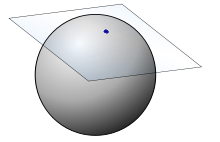
\includegraphics[width=0.3\textwidth]{5_Tangent_plane}
    \caption{A pictorial representation of the tangent space $T_xM$ of a single point, x, on a manifold. A vector in this $T_xM$ can represent a possible velocity at x. After moving in that direction to a nearby point, one's velocity would then be given by a vector in the tangent space of that nearby point — a different tangent space, not shown. \textit{By Alexwright at English Wikipedia - Transferred from en.wikipedia to Commons by Ylebru., Public Domain \url{https://commons.wikimedia.org/w/index.php?curid=3941393}}}
\end{SCfigure}

\begin{SCfigure}[5][h]
\label{fig:L5_TangentVector}
  \centering
    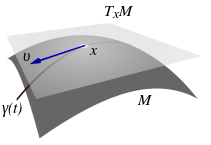
\includegraphics[width=0.3\textwidth]{5_Tangential_vector}
    \caption{The tangent space $T_xM$ and a tangent vector $v \in T_xM$, along a curve travelling through $x \in M$. \textit{By derivative work: McSush (talk)Tangentialvektor.png: TNThe original uploader was TN at German Wikipedia - Tangentialvektor.png, Public Domain, \url{https://commons.wikimedia.org/w/index.php?curid=4821938}}}
\end{SCfigure}

\textit{\textbf{Caution}: Although the Fig. \ref{fig:L5_TangentPlane} and \ref{fig:L5_TangentVector} refer to an ambient space in which $M$ is embedded, the tangent space has been defined intrinsically. There is a velocity corresponding to each curve along a different path in $M$ passing through $p$. Velocity along two different curves could be same, or curves along same paths but having different parameter speeds would yield different velocities.}

\begin{theorem}
$(T_pM, \oplus, \otimes)$ is a vector space with 
\begin{align*}
  \oplus : & T_pM \times T_pM \to Hom(C^\infty(M),\R)  \\
  & (v_{\gamma,p} \oplus v_{\delta,p})(\underbrace{f}_{ \in C^{\infty}(M)} ) := v_{\gamma,p}(f) +_{\R} v_{\delta,p}(f) \\
  \odot : & \R \times T_pM \to Hom(C^{\infty}(M),\R) \\
  & (\alpha \odot v_{\gamma,p} )(f) := \alpha \cdot_{\R}  v_{\gamma, p}(f)
\end{align*}
\end{theorem}

\begin{proof} Various conditions that must be satisfied by a vector space, are trivially satisfied. It remains to be shown that 
\begin{enumerate}[i)]
  \item For product, $\exists \, \tau $ curve : $\alpha \odot v_{\gamma,p} = v_{\tau,p}$
  \item For sum, $\exists \, \sigma$ curve : $v_{\gamma,p} \oplus v_{\delta,p} = v_{\sigma,p}$
\end{enumerate}
\underline{Product}: Let $\tau : \R \to M$ with $\lambda \mapsto \tau(\lambda) := \gamma(\alpha  \lambda + \lambda_0) = (\gamma \after \mu_{\alpha})(\lambda)$
where $\mu_{\alpha} : \R \to \R$ with $r \mapsto \alpha \cdot r + \lambda_0$. Then $\tau(0) = \gamma(\lambda_0) = p$, and
\[
v_{\tau,p} = (f \after \tau)^{\prime}(0) = (f \after \gamma \after \mu_{\alpha})^{\prime}(0) = \mu_{\alpha}^{\prime}(0) \cdot (f \after \gamma)^{\prime}(\mu_{\alpha}(0)) = \alpha \cdot (f \after \gamma)^{\prime}(\lambda_0) = \alpha \cdot v_{\gamma,p}
\]

\underline{Sum}: Choose a chart $(U,x)$ and $p \in U$. \textit{(If the proof will depend on the choice of a chart, alarm bells should ring. But we shall see that the result is finally independent of the chart.)} \\
Let $p = \gamma(\lambda_0) = \delta(\lambda_1)$. \\
Now define $\sigma : \R \to M$ with $\lambda \mapsto \sigma(\lambda) := x^{-1}(\underbrace{(x \after \gamma)(\lambda_0 + \lambda)}_{\R \to \R^d} + (x \after \delta)(\lambda_1 + \lambda) - (x \after \gamma)(\lambda_0))$. \\
Then, $\sigma_x(0) = x^{-1}((x \after \gamma)(\lambda_0) + (x \after \delta)(\lambda_1) - (x \after \gamma)(\lambda_0)) = \delta(\lambda_1) = p$. \\
Now
\begin{align*}
  v_{\sigma_x,p}(f) & := (f \after \sigma_x)^{\prime}(0) \\ 
  & = ( \underbrace{(f \after x^{-1})}_{\R^d \to \R} \after \underbrace{(x \after \sigma_x)}_{\R \to \R^d})^{\prime}(0) \\
  & = \underbrace{(x \after \sigma_x)^{\prime}(0)}_{(x \after \gamma)^{\prime}(\lambda_0) + (x \after \delta)^{\prime}(\lambda_1)} \cdot \left( \partial_i (f \after x^{-1}) \right)(x(\underbrace{\sigma(0)}_{p})) \\
  & = (x \after \gamma)^{\prime}(\lambda_0)(\partial_i (f \after x^{-1}))(x(p)) + (x \after \delta)(\lambda_1)(\partial_i (f \after x^{-1}))(x(p)) \\
  & = (f \after \gamma)^{\prime}(\lambda_0) + (f \after \delta)^{\prime}(\lambda_1) \\
  & = v_{\gamma,p}(f) + v_{\delta,p}(f) && \forall \, f \in C^{\infty}(M)
\end{align*}
\end{proof}

\textit{\textbf{Note}: If we push $\gamma$ and $\delta$ to one chart, and add them there, then bring the sum back to $M$, we would get a curve which would be different from the curve we would get if we used another chart. But it turns out, irrespective of the charts selected, we get the same tangent/velocity. Conclusion: Adding trajectories is chart dependent; hence, bad. Adding velocities is good because, whatever the charts, they yield the same derivative at the point of intersection. Of course, you cannot add two curves $(\gamma \oplus \delta)(\lambda) := \gamma(\lambda) +_M \delta(\lambda)$ because there is no addition $+_M$ in $M$. Defining $+$ through charts results in chart-dependent results, which is, therefore, not real.}  

\subsection{Components of a vector w.r.t. a chart}
\begin{tikzpicture}
  \matrix (m) [matrix of math nodes, row sep=4em, column sep=6em, minimum width=2em]
  {
    \R & M & \R \\
    & \R^d & \\
  };
  \path[->]
  (m-1-1) edge node[auto] {$\gamma$} (m-1-2)
          edge node[sloped, anchor=center, below] {$x \after \gamma$} (m-2-2)
  (m-1-2) edge node[auto] {$x$} (m-2-2)
          edge node[auto] {$f$} (m-1-3)
  (m-2-2) edge node[sloped, anchor=center, below] {$f \after x^{-1}$} (m-1-3);
\end{tikzpicture}

Let $(U,x) \in \A_{\text{smooth}}, \, \gamma : \R \to U$ and $\gamma(0) = p$. Then
\begin{align*}
  v_{\gamma,p}(f) & := (f \after \gamma)^\prime(0) \\
  & = (\underbrace{(f \after x^{-1})}_{\R^d \to \R} \after \underbrace{(x \after \gamma)}_{\R \to \R^d})^\prime(0) \\
  & = \displaystyle\left(\left(x \after \gamma\right)^\prime\right)^i(0) \cdot \left(f \after x^{-1}\right)^\prime_i(x(p)) \\
  & = \underbrace{\displaystyle\left(\left(x \after \gamma\right)^\prime\right)^i(0)}_{=: \dot{\gamma}_x^i(0)} \cdot \underbrace{(\partial_i(f \after x^{-1}))(x(p))}_{=: \left(\cibasis[f]{x^i}\right)_p} \\
  & = \dot{\gamma}_x^i(0) \cdot \left(\cibasis{x^i}\right)_p f && \forall \, f \in C^{\infty}(M), f : M \to \R
\end{align*}

\begin{definition}
For velocity $v_{\gamma,p}$, as a map under use of a chart $(U,x)$,
\begin{equation}\label{eq:defVelocityExpansion}
\boxed{v_{\gamma,p} = \dot{\gamma}_x^i(0) \cdot \left(\cibasis{x^i}\right)_p}
\end{equation} 
where
\begin{equation}\label{eq:defVelocityComponents}
\displaystyle\dot{\gamma}_x^i = \left(\left(x \after \gamma\right)^\prime\right)^i
\end{equation} 
are the \textbf{components of the velocity} $v_{\gamma,p}$ and
\begin{equation}\label{eq:defCIBasis}
\displaystyle\left(\cibasis{x^i}\right) = \partial_i\left(\,\cdot \after x^{-1}\right) = \left(\left(\, \cdot \after x^{-1}\right)^\prime\right)^i
\end{equation} 
which eat a function, form a basis of $T_pM$ w.r.t. which the components of the velocity need to be understood.
\end{definition}

\textit{Note: The components of a vector are always w.r.t. a chart. In $M$, there is just the vector, no components.} \\

\begin{theorem}
\label{thm:L5_dxiupondxj}
For a chart $(U,x)$,
\begin{equation}
\boxed{\cibasis[x^i]{x^j} = \delta^i_j}
\end{equation}
\end{theorem}
\begin{proof}
\begin{align*}
\cibasis[x^i]{x^j} = \partial_j (x^i \after x^{-1})(x(p)) = \delta^i_j && \text{(since } x^i \after x^{-1} : \R^d \to \R \text{ s.t. } (\alpha^1 , \dots , \alpha^d) \mapsto \alpha^i)
\end{align*}
\end{proof}

\subsection{Chart-induced basis}
\begin{definition}
If $(U,x) \in \A_{\text{smooth}}$, then $\displaystyle\left(\cibasis{x^1}\right)_p, \dotsc, \left(\cibasis{x^d}\right)_p \in T_pU \subseteq T_pM$ constitute a \textbf{chart-induced basis} of $T_pU$.
\end{definition}

\begin{proof} We have already shown that any vector in $T_pU$ can be expressed in terms of $\displaystyle\left(\cibasis{x^i}\right)_p$. It remains to be shown that they are linearly independent. That is, we require $\displaystyle\lambda^i \left(\cibasis{x^i}\right)_p = 0 \implies \lambda^i = 0$ for all $i = 1, \dotsc, d$. Or,
\begin{align*}
0 & = \lambda^i \left(\cibasis{x^i}\right)_p(x^j) && x^j : U \to \R \text{ is differentiable}\\
& = \lambda^i \partial_i (x^j \after x^{-1})(x(p)) && \text{by Eq. \ref{eq:defCIBasis}} \\
& = \lambda^i \delta^j_i && \text{by Theorem \ref{thm:L5_dxiupondxj}} \\
& = \lambda^j && \text{for all } j = 1, \dotsc, d 
\end{align*}
\end{proof}

\begin{corollary}
$dim \, T_pM = d = dim \, M$. \\
This follows from the fact $d$ vectors are needed to express any vector in $T_pM$, and these $d$ vectors arise from the $d$ coordinates of chart which shows that $M$ has $d$ dimensions.
\end{corollary}

\underline{Terminology}: $X \in T_pM \implies \exists \, \gamma : \R \to M : X = v_{\gamma,p}$ and $\displaystyle \exists \, \underbrace{X^1, \dotsc, X^d}_{\in \R} : X = X^i \left(\cibasis{x^i}\right)_p$. $X^i$ are called \textbf{components of the vector $X$ w.r.t chart-induced basis}.

\subsection{Change of vector components under a change of chart}
\ding{56} A vector does not change under change of chart; only the vector components do.

Let $(U,x)$ and $(V,y)$ be overlapping charts and $p \in U \cap V$. Let $X \in T_pM$. Then, $X$ can be expanded in terms of chart-induced basis of the two charts as follows:
\begin{equation}\label{eq:L5_VecExpandedIn2Charts}
X^i_{(y)} \cdot \left(\cibasis{y^i}\right)_p \underbrace{=}_{(V,y)} X \underbrace{=}_{(U,x)} X^i_{(x)} \cdot \left(\cibasis{x^i}\right)_p
\end{equation}
\begin{align*}
  \text{Now, } \quad \quad \left(\cibasis{x^i}\right)_p f & = \partial_i(f \after x^{-1})(x(p)) \\
  & = \partial_i (\underbrace{(f \after y^{-1})}_{\R^d \to \R} \after (\underbrace{y \after x^{-1}}_{\R^d \to \R^d})(x(p)) \\
  & = (\partial_i (y \after x^{-1})^j)(x(p)) \cdot (\partial_j (f \after y^{-1}))(y(p)) \\
  & = (\partial_i (y^j \after x^{-1}))(x(p)) \cdot (\partial_j (f \after y^{-1}))(y(p)) \\
  & = \boxed{\left(\cibasis[y^j]{x^i}\right)_p \cdot \left(\cibasis[f]{y^j}\right)_p}
\end{align*}

\begin{equation}\label{eq:L5_cibasisIn2Charts}
\therefore \boxed{\left(\cibasis{x^i}\right)_p = \left(\cibasis[y^j]{x^i}\right)_p \cdot \left(\cibasis{y^j}\right)_p}
\end{equation}
Using Eq. \ref{eq:L5_VecExpandedIn2Charts} and Eq. \ref{eq:L5_cibasisIn2Charts}, 
\[
  X^i_{(x)} \left(\cibasis[y^j]{x^i}\right)_p \left(\cibasis{y^j}\right)_p = X^j_{(y)}\left(\cibasis{y^j}\right)_p
\]
\begin{equation}
\therefore \boxed{X^j_{(y)} = \left(\cibasis[y^j]{x^i}\right)_p X^i_{(x)}}
\end{equation}

\subsection{Cotangent spaces}
% \url{https://youtu.be/pepU_7NJSGM?t=1h24m36s}
Since $T_pM$ is a vector space, therefore it is trivial to define cotangent space as follows.

\begin{definition}
For the tangent space $T_pM$ at $p \in M$, \textbf{cotangent space} is defined as
\begin{equation}
(T_pM)^* := \lbrace \varphi : T_pM \linearmapto \R \rbrace
\end{equation}
\end{definition}

\begin{definition}
\label{def:gradient}
If $f \in C^{\infty}(M)$, then the \textbf{gradient of $f$ at the point $p \in M$} is defined as
\begin{align}
\label{eq:defGradient}
  (df)_p : & T_p M \linearmapto \R \nonumber \\ 
  & X \mapsto (df)_p(X) := Xf
\end{align}

\end{definition}
i.e. $\boxed{(df)_p \in T_pM^*}$

$(df)_p$ is a $(0,1)$-tensor over the underlying vector space $T_pM$. We define the components of the gradient the same way as we define the components of a tensor (refer section \ref{ss:L3_TensorComponents}).

\begin{definition}
\textbf{Components of gradient w.r.t. chart-induced basis of $(U,x)$} are defined as
\begin{equation}
\left((df)_p \right)_j := (df)_p\left(\left(\cibasis{x^j}\right)_p \right) = \left(\cibasis[f]{x^j}\right)_p = \partial_j (f \after x^{-1})(x(p))
\end{equation}
\end{definition}

\begin{theorem}
A chart $(U,x) \implies x^i : U \to \R$ are smooth functions. Then, $(dx^1)_p, (dx^2)_p, \dotsc, (dx^d)_p$ form a basis of $T_p^*M$. 
\end{theorem}
\begin{proof}
In fact, $(dx^i)_p$ form a dual basis since 
\begin{equation}
(dx^a)_p \left(\left(\cibasis{x^b}\right)_p \right) = \left(\cibasis[x^a]{x^b}\right)_p = \delta_b^a \textit{ (using Theorem \ref{thm:L5_dxiupondxj})}
\end{equation}
\end{proof}

\subsection{Change of components of a covector under a change of chart}
\ding{56} A covector does not change under change of chart; only the covector components do.

Let $(U,x)$ and $(V,y)$ be overlapping charts and $p \in U \cap V$. Let $\omega \in T_p^*M$. Then, $\omega$ can be expanded in terms of chart-induced basis of the two charts as follows:
\begin{equation}\label{eq:L5_CovecExpandedIn2Charts}
\displaystyle\omega_{(y)k}(dy^k)_p \underbrace{=}_{(V,y)} \omega \underbrace{=}_{(U,x)} \omega_{(x)j}(dx^j)_p
\end{equation}
\begin{align*}
  \implies && \displaystyle\omega_{(y)k}(dy^k)_p \left(\cibasis{y^i}\right)_p & = \omega_{(x)j}(dx^j)_p \left(\cibasis{y^i}\right)_p \\
  \implies && \displaystyle\omega_{(y)k} \left(\cibasis[y^k]{y^i}\right)_p & = \omega_{(x)j} \left(\cibasis[x^j]{y^i}\right)_p && \text{by Eq. \ref{eq:defGradient}} \\
  \implies && \displaystyle\omega_{(y)k} \delta^k_i & = \omega_{(x)j} \left(\cibasis[x^j]{y^i}\right)_p && \text{by Theorem \ref{thm:L5_dxiupondxj}}
\end{align*}
\begin{align}
\implies && \boxed{\omega_{(y)i} = \left(\cibasis[x^j]{y^i}\right)_p \omega_{(x)j}} &&
\end{align}

%\begin{align*}
%\implies && \omega_{(y)i}(dy^i)_p & = \left(\cibasis[x^j]{y^i}\right)_p \omega_{(x)j}(dy^i)_p \\
%\implies && \omega & = \left(\cibasis[x^j]{y^i}\right)_p \omega_{(x)j}(dy^i)_p \\
%\implies && \omega (dx^j)_p & = \left(\cibasis[x^j]{y^i}\right)_p \omega_{(x)j}(dy^i)_p (dx^j)_p \\
%\implies && \omega (dx^j)_p & = \left(\cibasis[x^j]{y^i}\right)_p \omega (dy^i)_p \\
%\implies && (dx^j)_p & = \left(\cibasis[x^j]{y^i}\right)_p (dy^i)_p
%\end{align*}
%
%\begin{equation}\label{eq:L5_cicobasisIn2Charts}
%\therefore \boxed{(dx^j)_p = \left(\cibasis[x^j]{y^i}\right)_p (dy^i)_p}
%\end{equation}
 % Tangent Spaces

\section{Fields}

So far, we have focussed technically on a single tangent space and a vector/ covector in it, a basis if we chose a chart. As physicists, we are interested in things such as vector fields such that at any point of a manifold, there is a vector. The proper way to deal with it technically is \textit{theory of bundles}.

\subsection{Bundles}

\begin{definition}
A \textbf{bundle} is a triple $\boxed{E \projmapto M}$, where \\
$E$ is a smooth manifold, called the \textbf{total space}, \\
$M$ is a smooth manifold, called the \textbf{base space}, and \\
$\pi$ is a smooth map (surjective), called the \textbf{projection map}. \\
\end{definition}

\begin{definition}
Let $E \projmapto M$ be a bundle and $p \in M$. Then, \textbf{fibre over} $p := \text{preim}_{\pi}(\lbrace p \rbrace)$. \\
\end{definition}

\begin{definition}
A \textbf{section} $\sigma$ of a bundle $E \projmapto M$ is the map $\sigma : M \to E$ such that $\pi \after \sigma = id_M$. \\
\end{definition}

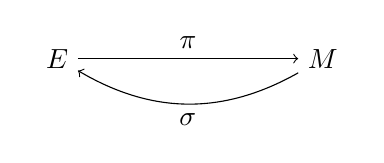
\begin{tikzpicture}
  \matrix (m) [matrix of math nodes, row sep=3em, column sep=8em, minimum width=1em]
  { E & M \\ };
  \path[->]
  (m-1-1) edge node [above] {$\pi$} (m-1-2)
  (m-1-2) edge [bend left=30] node [below] {$\sigma$} (m-1-1);
\end{tikzpicture}

\underline{Example}: $E$ is a cylinder, $M$ a circle and $\pi$ maps vertical lines on the cylinder to the point of intersection of this line with the circle.

\underline{Example}: If the fibre of $p \in M$ is a tangent space, the section would pick one vector from the tangent space.

\underline{Aside}: In quantum mechanics, $\psi : M \to \mathbb{C}$ is called a wavefunction, but it is actually a section which selects one value from $\mathbb{C}$ for each $p \in M$.


\subsection{Tangent bundle of smooth manifold}
For this entire subsection, let $\mfd$ be a smooth manifold and let $d := dim \, M$. 

Define the set, 
\begin{equation}
\boxed{TM : = \dot{\bigcup}_{p \in M} T_pM}
\end{equation}

Now define a surjective map $\pi$ as follows:
\begin{equation}
\boxed{\begin{split}
  \pi : & TM \to M \\
  & X \mapsto \pi(X) := p \in M \text{ such that } X \in T_pM
\end{split}}
\end{equation}

\underline{Situation}:  $\underbrace{TM}_{\text{set}} \underbrace{ \projmapto}_{\text{surjective map}} \underbrace{M}_{\text{smooth manifold}}$

For a bundle, $TM$ should be a smooth manifold and $\pi$ a smooth map. Let us construct a topology on $TM$ that is the coarsest topology such that $\pi$ is just continuous. (\textbf{initial topology} with respect to $\pi$). Define

\begin{equation}
\boxed{\mathcal{O}_{TM} := \lbrace \text{preim}_{\pi}(U) | U \in \mathcal{O} \rbrace}
\end{equation}

It can be shown that $(TM,\mathcal{O}_{TM})$ is a topological space. But we need a smooth atlas.\\

\underline{Construction of a $C^{\infty}$-atlas on $TM$ from the $C^{\infty}$-atlas $\A$ on $M$} \\
Define
\begin{equation}\label{eq:atlasTangentBundle}
\boxed{
\begin{split}
\A_{TM} := & \lbrace (TU,\xi_x) \, | \, (U,x) \in \A \rbrace \text{ where } \\
  \xi_x : & TU \to \R^{2d} \\
  & X \mapsto \left(\underbrace{(x^1 \after \pi)(X), \dotsc, (x^d \after \pi)(X)}_{(U,x)-\text{ coords of } \pi(X) \, (d\text{-many})}, \underbrace{(dx^1)_{\pi(X)}(X), \dotsc, (dx^d)_{\pi(X)}(X)}_{\text{components of $X$ w.r.t } (U,x) \, (d\text{-many})}\right)
\end{split}
}
\end{equation}

In the above, $(x^1 \after \pi)(X) = x^1(\pi(X)) = x^1(p) = x^1 \text{-coordinate}$, and \\
$X \in T_{\pi(X)}M \implies X = X_{(x)}^i \left(\cibasis{x^i}\right)_{\pi(X)} \implies (dx^j)_{\pi(X)}(X) = (dx^j)_{\pi(X)} \left(X^i_{(x)}\left(\cibasis{x^i}\right)_{\pi(X)} \right) = X^i_{(x)}\delta_i^j = X^j_{(x)}$. \\
Thus $\xi_x$ maps $X$ to the coordinates of its base point $\pi(X)$ under the chart $(U,x)$ and the components of the vector $X$ w.r.t the basis induced by this chart.

We can write $\xi_x^{-1}$ as follows:
\begin{equation}\label{eq:xiInverseTangentBundle}
\boxed{
\begin{split}
\xi_x^{-1} \, : \, & \underbrace{\xi_x(TU)}_{\subseteq \R^{2d}} \to TU \\
& (\alpha^1, \dotsc, \alpha^d, \beta^1, \dotsc, \beta^d) := \beta^i \left(\cibasis{x^i}\right)_{\underbrace{x^{-1}(\alpha^1, \dotsc, \alpha^d)}_{\pi(X)}}
\end{split}
}
\end{equation}

Now we check, whether the atlas $\A_{TM}$ smooth. That is, are the transitions between its charts smooth?

\begin{theorem}
$\A_{TM}$ is a smooth atlas.
\end{theorem}

\begin{proof}
Let $(U,\xi_x) \in \A_{TM}, \quad (V,\xi_y) \in \A_{TM} \quad \text{ and } \quad U \cap V \ne \emptyset$. Calculate the chart transition
\begin{align*}
& (\xi_y \after \xi_x^{-1})(\alpha^1, \dotsc, \alpha^d, \beta^1, \dotsc, \beta^d) = \xi_y \left(\beta^i \left(\cibasis{x^i} \right)_{x^{-1}(\alpha^1, \dotsc, \alpha^d)}\right) && \text{by Eq.~\ref{eq:xiInverseTangentBundle}} \\
& = \left(\dotsc, (y^i \after \pi)\left(\beta^m \cdot \left(\cibasis{x^m}\right)_{x^{-1}(\alpha^1, \dotsc, \alpha^d)}\right), \dotsc, \dotsc, (dy^i)_{x^{-1}(\alpha^1, \dotsc, \alpha^d)} \left(\beta^m \left(\cibasis{x^m} \right)_{x^{-1}(\alpha^1, \dotsc, \alpha^d)} \right), \dotsc \right) && \text{by Eq.~\ref{eq:atlasTangentBundle}}  \\
& = \left(\dotsc, y^i \left(\underbrace{\pi\left(\beta^m \cdot \left(\cibasis{x^m}\right)_{x^{-1}(\alpha^1, \dotsc, \alpha^d)}\right)}_{\text{the base point,}\, x^{-1}(\alpha^1, \dotsc, \alpha^d)}\right), \dotsc, \dotsc, (\beta^m \underbrace{(dy^i)_{x^{-1} (\alpha^1, \dotsc, \alpha^d)} \left( \left(\cibasis{x^m}\right)_{x^{-1}(\alpha^1, \dotsc, \alpha^d)} \right)}_{\left(\cibasis[y^i]{x^m}\right)_{x^{-1}(\alpha^1, \dotsc, \alpha^d)}}, \dotsc \right) \\
& = \left(\dotsc, (y^i \after x^{-1})(\alpha^1, \dotsc, \alpha^d), \dotsc, \dotsc, \beta^m \left(\left(\cibasis[y^i]{x^m}\right)_{x^{-1}(\alpha^1, \dotsc, \alpha^d)} \right), \dotsc\right) \\
& = \left(\dotsc, (y^i \after x^{-1})(\alpha^1, \dotsc, \alpha^d), \dotsc, \dotsc, \beta^m \left(\partial_m (y^i \after x^{-1})( x (x^{-1}(\alpha^1, \dotsc, \alpha^d))) \right), \dotsc\right) \\
& = \left(\dotsc, \underbrace{(y^i \after x^{-1})(\alpha^1, \dotsc, \alpha^d)}_{\text{smooth } \because \mathcal(A) \text{ is smooth atlas}}, \dotsc, \dotsc, \underbrace{\beta^m \left(\partial_m (y^i \after x^{-1})(\alpha^1, \dotsc, \alpha^d)\right)}_{\text{smooth } \because \text{ chart transition map is } C^\infty \text{ smooth}}, \dotsc\right) \\
& \implies (\xi_y \after \xi_x^{-1}) \text{ is smooth} \implies \A_{TM} \text{ is smooth}
\end{align*}
\end{proof}

Further, the surjective map $\pi$ is a smooth map because, in the chart representation, $\pi$ takes the $2d$ components of $X \in TM$ to the $d$-coordinates of the base point in $M$, which can be seen to happen smoothly by seeing how the components are mapped. Therefore, we have the following definition. 
\begin{definition}
Then, using the smooth manifold $\mfd$ as the base space and the smooth manifold $(TM, \mathcal{O}_{TM}, \A_{TM})$ as the total space, the \textbf{tangent bundle} is the triple
\begin{equation}\label{eq:TangentBundle}
\boxed{TM \projmapto M}
\end{equation}
\end{definition}

\subsection{Vector fields}
Why did we put so much effort in making a smooth atlas on $TM$ and defining a tangent bundle? The answer is in the following definition of \emph{smooth} vector field, not just any vector field.

\begin{definition}
For a tangent bundle $TM \projmapto M$, a \textbf{smooth vector field} $\chi$ is a smooth map such that $\pi \after \chi = id_{M}$.
\end{definition}

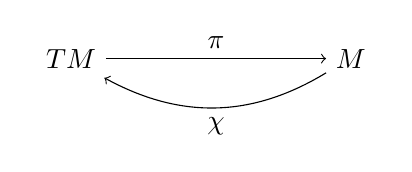
\begin{tikzpicture}
  \matrix (m) [matrix of math nodes, row sep=3em, column sep=8em, minimum width=1em]
  { TM & M \\ };
  \path[->]
  (m-1-1) edge node [above] {$\pi$} (m-1-2)
  (m-1-2) edge [bend left=30] node [below] {$\chi$} (m-1-1);
\end{tikzpicture}

\textit{Remarks: $\chi$ is a section, which couldn't have been a smooth map unless we had both $M$ and $TM$ as smooth manifolds.}

\subsection{The $C^{\infty}(M)$-module $\Gamma(TM)$}
We already know that $C^{\infty}(M)$, the collection of all smooth functions is a vector space with S-multiplication with $\R$. But we may also consider the structure $(C^{\infty}(M),+,\cdot)$ with point-wise addition between elements of $C^{\infty}(M)$ and point-wise multiplication between elements of $C^{\infty}(M)$. This structure satisfies all the requirements of a field (commutativity, associativity, neutral element, inverse element under both operations, and distributivity) except that there is no inverse for all non-zero elements under multiplication. This is so because a function that is not zero everywhere, may be zero at some points and then point-wise multiplication with no function would result in the value 1 everywhere. Such a structure is called a ring. 

A module over a ring is a generalization of the notion of vector space over a field, wherein the corresponding scalars are the elements of an arbitrary given ring.

Let us consider the module made from the set of all smooth vector fields over the ring $C^{\infty}(M)$. Define \\
\begin{equation}
\Gamma(TM) = \lbrace \chi \, : \, M \to TM \, | \, \chi \text{ is a smooth section} \rbrace
\end{equation}

\begin{definition}
$(\Gamma(TM),\oplus,\odot)$ is a $C^{\infty}(M)$-module over the ring of $C^{\infty}(M)$ functions with $\chi, \widetilde{\chi} \in \Gamma(TM)$ and $g \in C^{\infty}(M)$, such that \\
$(\chi \oplus \widetilde{\chi})(f) := (\chi f) \underbrace{+}_{C^{\infty}(M)} (\widetilde{\chi}f)$ \\
$(g \odot \chi)(f) := g \underbrace{\cdot}_{C^{\infty}(M)} (\chi f)$
\end{definition}

\underline{Facts}: Besides other differences, there are following 2 important facts:
\begin{enumerate}
\item[(1)] Proving that \textit{every vector space has a basis} depends upon the choice of set theory; in particular, on the Axiom of Choice in ZFC theory.
\item[(2)] No such result exists for modules.  
\end{enumerate}

This is a shame, because otherwise, we could have chosen (for any manifold) vector fields, $\chi_{(1)}, \dotsc, \chi_{(d)} \in \Gamma(TM)$ and would be able to write every vector field $\chi$ in terms of component functions $f^i$ as $\chi = f^i \cdot \chi_{(i)}$.

\textbf{Simple counterexample:} Take a sphere. Can we find a smooth vector field over the entire sphere. Can you comb the sphere? No. For the field to be smooth, there is a problem. Morse Theory tells us that every smooth vector field on a sphere must vanish at 2 points $\implies$ basis cannot be chosen. We cannot choose a global basis. Therefore, if required, we only expand a vector field in terms of a basis on a domain where it is possible.


\textit{Remarks: Although we cannot have a global basis for $\Gamma(TM)$, it is possible to do so locally. Thus, for the chart $(U,x)$ we can take the \textbf{chart-induced basis of the vector field} in the chart domain $U$ as the map \\
\begin{equation}
\begin{split}
  \cibasis{x^i} : & \, U \xrightarrow{\text{ smooth }} TU \\
  & p \mapsto \left(\cibasis{x^i}\right)_p
\end{split}
\end{equation}
}

\subsection{Tensor fields}
So far we have constructed the sections over the tangent bundle. That is, $\Gamma(TM) = $''set of smooth vector fields'' as a $C^{\infty}(M)$-module.

Exactly along the same lines we can construct the \textbf{cotangent bundle} $\Gamma(T^*M) = $ ``set of covector fields'' as a $C^{\infty}(M)$-module, by mapping a covector to the coordinates of its base point and components of the covector. $\Gamma(TM)$ and $\Gamma(T^*M)$ are the basic building blocks for every tensor field.

\begin{definition}
An \textbf{$(r,s)$-tensor field} $T$ is a multilinear map
\begin{equation}
T:\underbrace{\Gamma(T^*M) \times \dotsb \times \Gamma(T^*M)}_{r} \times \underbrace{\Gamma(TM) \times \dotsb \times \Gamma(TM)}_{s} \linearmapto C^{\infty}(M)
\end{equation}
\end{definition}

\textit{Remarks: the multilinearity is in $C^{\infty}(M)$, in terms of addition in the modules and S-multiplication with functions in $C^{\infty}(M)$.}

\textbf{Example:} Let $f\in C^{\infty}(M)$. Then, define a ($0,1$)-tensor field $df$ as
\[
\begin{gathered}
  \begin{aligned} 
    df : & \Gamma(TM) \linearmapto C^{\infty}(M) \\ 
    & \chi \mapsto df(\chi) := \chi f && \text{ such that } (\chi f)(\underbrace{p}_{ \in M}) := \underbrace{\chi(p)}_{\in T_pM}f
\end{aligned}
\end{gathered}
\]
It can be checked that $df$ is $C^{\infty}-$linear.
 % Fields

\section{Lecture 7: Connections}
\begin{framed}
\textbf{Motivation}: So far, all we have dealt with (e.g., sets, topological manifolds, smooth manifolds, fields, bundles, etc.) are structures that we have to provide by hand before we can start doing physics as we know it. Why? Because we don't have equations which determine what we have done so far. These are assumptions you need to submit before you can do physics.

In this lecture we introduce yet another structure called connections which are determined by Einstein's equations. Everything from now on will be objects that are the subject of Einstein's equations depending on the matter in the Universe. Connections are also called covariant derivatives. Even though these are different, for our purposes we shall not distinguish the two and use the more general connections.
\end{framed}

So far, we saw that a vector field $X$ can be used to provide a directional derivative of a function $f \in C^{\infty}(M)$ in the direction $X$\\
\begin{equation*}
\nabla_X f := Xf
\end{equation*}
Isn't this a notational overkill? We already know \\
\begin{equation*}
\nabla_X f = Xf = (df)X
\end{equation*}
Actually, they are not quite the same because
\[
\begin{aligned}
  X : C^{\infty}(M) \to C^{\infty}(M) \\ 
  df : \Gamma(TM) \to C^{\infty}(M) \\
  \nabla_X : C^{\infty}(M) \to C^{\infty}(M)
\end{aligned}
\]
where $\nabla_X$ can be generalized to eat an arbitrary $(p,q)$-tensor field and yield a $(p,q)$-tensor field whereas $X$ can only eat functions. \\
\[
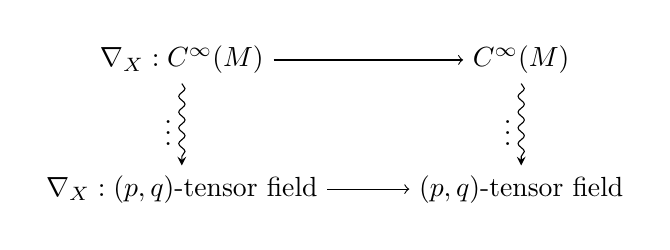
\begin{tikzpicture}
\matrix (m) [matrix of nodes, row sep=3em, column sep=3em, minimum width=1em]
{
$\nabla_X : C^{\infty}(M)$ & $C^{\infty}(M)$ \\
$\nabla_X : (p,q)$-tensor field & $(p,q)$-tensor field \\ };
\path[->]
  (m-1-1) edge (m-1-2);
\path[->]
  (m-2-1) edge (m-2-2);
\path[->]
  (m-1-1) edge[snake it] node[left] {$\vdots$} (m-2-1);
\path[->]
  (m-1-2) edge[snake it] node[left] {$\vdots$} (m-2-2);
\end{tikzpicture}
\]

We need $\nabla_X$ to provide the new structure to allow us to talk about directional derivatives of tensor fields and vector fields. Of course, only in cases where $\nabla_X$ acts on function $f$ which is a $(0,0)$-tensor, it is exactly the same as $Xf$. 

\subsection{Directional derivatives of tensor fields}
We formulate a wish list of properties which $\nabla_X$ acting on a tensor field should have. We put this in form of a definition. There may be many structures that satify this wish list. Any remaining freedom in choosing such a $\nabla$ will need to be provided as additional structure beyond the structure we already have. And we assume all this takes place on a smooth manifold.

\begin{definition}\label{def:connection}
A \textbf{connection} $\nabla$ on a smooth manifold $(M, \mathcal{O}, \mathcal{A})$ is a map that takes a pair consisting of a vector (field) $X$ and a $(p,q)$-tensor field $T$ and sends them to a $(p,q)$-tensor (field) $\nabla_X T$ satisfying
\begin{enumerate}[i)]
\item $\nabla_X f = Xf \quad \forall f \in C^{\infty}M$

\item $\nabla_X (T + S) = \nabla_X T + \nabla_X S \quad \text{ where }T, S \text{ are } (p,q) \text{-tensors}$

\item \textbf{Leibnitz rule: } $\nabla_X T(\omega_1,\dotsc,\omega_p,Y_1,\dotsc,Y_q) = (\nabla_X T)(\omega_1,\dotsc,\omega_p,Y_1,\dotsc,Y_q) \\
+ T(\nabla_X \omega_1,\dotsc,\omega_p,Y_1,\dotsc,Y_q) + \dotsb + T(\omega_1,\dotsc,\nabla_X \omega_p,Y_1,\dotsc,Y_q) \\
+ T(\omega_1,\dotsc,\omega_p,\nabla_X Y_1,\dotsc,Y_q) + \dotsb + T(\omega_1,\dotsc,\omega_p,Y_1,\dotsc,\nabla_X Y_q) \quad \text{ where }T \text{ is a }(p,q)\text{-tensor}$
\begin{framed}
Note that for a $(p,q)$-tensor $T$ and a $(r,s)$-tensor $S$, since: \\
$(T \otimes S) (\omega_{(1)}, \dotsc, \omega_{(p+r)}, Y_{(1)}, \dotsc, Y_{(q+s)}) = \\ T(\omega_{(1)}, \dotsc, \omega_{(p)}, Y_{(1)}, \dotsc, Y_{(q)} ) \cdot S( \omega_{(p+1)}, \dotsc, \omega_{(p+r)} , Y_{(q+1)}, \dotsc, Y_{(q+s)})$, \\
Leibnitz rule implies $\nabla_X (T \otimes S) = (\nabla_X T) \otimes S + T \otimes (\nabla_X S)$.
\end{framed}

\item \textbf{$C^{\infty}$-linearity: }$\forall f \in C^{\infty}(M), \nabla_{fX+Z} T = f\nabla_X T + \nabla_Z T$
\begin{framed}
$C^{\infty}$-linearity means that no matter how the function $f$ scales the vectors at different points of the manifold, the effect of the scaling at any point is independent of scaling in the neighbourhood and depends only on how the scaling happens at that point.
\end{framed}
\end{enumerate}
\end{definition}

A \textbf{manifold with a connection} $\nabla$ is a quadruple $(M, \mathcal{O}, \mathcal{A}, \nabla)$, where $M$ is a set, $\mathcal{O}$ is a topology and $\mathcal{A}$ is a smooth atlas.

Remark: If $\nabla_X (\cdot)$ can be seen as an extension of $X$, \\
then $\nabla_{(\cdot)}(\cdot)$ can be seen as an extension of $d$.

\subsection{New structure on $(M,\mathcal{O},\mathcal{A})$ required to fix $\nabla$}
How much freedom do we have in choosing such a structure?

Consider vector fields $X, Y$ and chart $(U,x) \in \mathcal{A}$. Then \\
\begin{align*}
\nabla_X Y & = \nabla_{\left(X^i \cibasis{x^i}\right)} \left(Y^m \cibasis{x^m}\right) && \text{by expanding in chart-induced basis} \\
& = X^i \cdot \nabla_{\left(\cibasis{x^i}\right)} \left(Y^m \cibasis{x^m}\right) && \text{by }C^\infty\text{-linearity} \\
& = X^i \underbrace{\left(\nabla_{\left(\cibasis{x^i}\right)} Y^m\right)}_{=\cibasis{x^i} Y^m} \cibasis{x^m} + X^i \cdot Y^m \cdot \underbrace{\left(\nabla_{\left(\cibasis{x^i}\right)} \cibasis{x^m}\right)}_{\text{a vector field, by defn.}} && \text{using Leibnitz rule} \\
& =  X^i \left(\cibasis{x^i} Y^m\right) \cibasis{x^m} + X^i \cdot Y^m \cdot \left(\ccf{q}{mi} \cibasis{x^q}\right)
\end{align*}

Thus, by change of indices, 
\begin{equation}
\boxed{\left(\nabla_X Y\right)^i = X^m \left(\cibasis{x^m} Y^i\right) + X^m \cdot Y^n \cdot \ccf{i}{nm}}
\end{equation}
So we need $(dim\,M)^3$-many functions to define directional derivative of a vector field.

\begin{definition}
Given $(M, \mathcal{O}, \mathcal{A}, \nabla)$ and $(U,x) \in \mathcal{A}$, then the \textbf{connection coefficient functions} ($\Gamma$s) on $M$ of $\nabla$ w.r.t $(U,x)$ are $(dim\,M)^3$-many functions given by
\begin{align}
\ccf{i}{jk} : \quad & U \to \mathbb{R} \nonumber \\ 
& p \mapsto \ccf{i}{jk}(p) := \left(dx^i \left(\nabla_{\left(\cibasis{x^k}\right)} \cibasis{x^j}\right)\right)(p)
\end{align}
\end{definition}

\textit{Note: $\cibasis{x^j}$ is a vector field; $\therefore\,\nabla_{\left(\cibasis{x^k}\right)} \cibasis{x^j}$ is a vector field, and $dx^i$ is a covector which will result in a function after acting on a vector field.}

On a chart domain $U$, choice of the $(dim\,M)^3$-many functions $\ccf{i}{jk}$ suffices to fix the action of $\nabla$ on a vector field. What about the directional derivative of a covector field, or a tensor field? Will we have to provide more and more coefficients? Fortunately, the same $(dim\,M)^3$-many functions fix the action of $\nabla$ on any tensor field.

We know that, for a covector, $\nabla_{\cibasis{x^m}}\left(dx^i\right) = \Sigma\indices{^{i}_{jm}} dx^j$, since $dx^i$ form a dual basis. Are these $\Sigma$s independent of $\Gamma$s? Consider the following.

\begin{align*}
& \displaystyle\nabla_{\cibasis{x^m}} \left(dx^i \left(\cibasis{x^j}\right)\right) = \nabla_{\cibasis{x^m}} \delta^i_j = \cibasis{x^m}(\delta^i_j) = 0 \\
& \implies \displaystyle\left(\nabla_{\cibasis{x^m}} dx^i \right)\left(\cibasis{x^j}\right) + dx^i \underbrace{\left(\nabla_{\cibasis{x^m}} \cibasis{x^j}\right)}_{\ccf{q}{jm}\cibasis{x^q}} = 0 \\
& \implies \displaystyle\left(\nabla_{\cibasis{x^m}} dx^i \right)\left(\cibasis{x^j}\right) + dx^i \ccf{q}{jm} \cibasis{x^q} = 0 \\
& \implies \left(\nabla_{\cibasis{x^m}} dx^i \right)\left(\cibasis{x^j}\right) = - dx^i \ccf{q}{jm} \cibasis{x^q} = - \ccf{q}{jm} dx^i \cibasis{x^q} = - \ccf{q}{jm} \delta^i_q = - \ccf{i}{jm} \\
& \implies \left(\nabla_{\cibasis{x^m}} dx^i \right)\underbrace{\left(\cibasis{x^j}\right) dx^j}_{= \delta^j_j = 1} = -\ccf{i}{jm} dx^j \\
& \implies \boxed{\nabla_{\cibasis{x^m}} dx^i = -\ccf{i}{jm} dx^j} \\
& \implies \boxed{\left(\nabla_{\cibasis{x^m}} dx^i\right)_j = -\ccf{i}{jm}}
\end{align*}

In summary,
\begin{align}
  \displaystyle\left(\nabla_X Y\right)^i & = X(Y^i) + \ccf{i}{jm} Y^j X^m \\
  \displaystyle\left(\nabla_X \omega\right)_i & = X\left(\omega_i\right) - \ccf{j}{im} \omega_j X^m
\end{align}
Note that for the immediately above expression for $(\nabla_X Y)^i$, in the second term on the right hand side, $\ccf{i}{jm}$ has the last entry at the bottom, $m$ going in the direction of $X$, so that it matches up with $X^m$. This is a good mnemonic to memorize the index positions of $\ccf{}{}$.

Similarly, as an example, by further application of Leibnitz rule, for a $(1,2)$-tensor field $T$,
\begin{align*}
  \left(\nabla_X T\right)\indices{^i_{jk}} = X\left(T\indices{^i_{jk}}\right) + \ccf{i}{sm} T\indices{^s_{jk}} X^m - \ccf{s}{jm} T\indices{^i_{sk}} X^m - \ccf{s}{km} T\indices{^i_{js}} X^m
\end{align*}

%Student's Question: If in a Euclidean space, do the $\Gamma$s all vanish in a global chart? Yes, it is so by definition. But what is a Euclidean space? \\
%$\left(M = \mathbb{R}^n, \mathcal{O}_{\text{st}}, \mathcal{A}\right)$ smooth manifold. \\
%Assume $(\mathbb{R}^n, \text{id}_{\mathbb{R}^n} ) \in \mathcal{A}$ and 
%\[
%\ccfx{i}{jk}{(x)} = dx^i \left( (\nabla_{\text{\underline{E}}})_{\cibasis{x^k}}\cibasis{x^j} \right) \overset{!}{=} 0 
%\]

\subsection{Change of $\Gamma$'s under change of chart}
Let $(U,x)$, $(V,y) \in \mathcal{A}$ and $U \cap V \neq \emptyset$.

\begin{align*}
\ccfx{i}{jk}{(y)} & := dy^i \left(\nabla_{\cibasis{y^k}} \cibasis{y^j} \right) \\
& = \cibasis[y^i]{x^q} dx^q \left(\nabla_{\cibasis[x^p]{y^k} \cibasis{x^p}} \cibasis[x^s]{y^j} \cibasis{x^s} \right) \\
& = \cibasis[y^i]{x^q} dx^q \left(\cibasis[x^p]{y^k} \left[ \left(\nabla_{\cibasis{x^p}} \cibasis[x^s]{y^j} \right) \cibasis{x^s} + \cibasis[x^s]{y^j} \left(\nabla_{\cibasis{x^p}} \cibasis{x^s} \right) \right] \right) && \because \nabla \text{ is } C^{\infty}-linear \\
& = \cibasis[y^i]{x^q} \underbrace{\cibasis[x^p]{y^k} \cibasis{x^p}}_{\cibasis{y^k}} \cibasis[x^s]{y^j} \delta^q_s + \cibasis[y^i]{x^q} \cibasis[x^p]{y^k} \cibasis[x^s]{y^j} \ccfx{q}{sp}{(x)}
\end{align*}

\begin{equation}\label{Eq:WEHCG0703_changeofGamma}
\ccfx{i}{jk}{(y)} = \cibasis[y^i]{x^q} \frac{\partial^2 x^q}{\partial y^k \partial y^j} + \cibasis[y^i]{x^q} \cibasis[x^s]{y^j} \cibasis[x^p]{y^k} \ccfx{q}{sp}{(x)}
\end{equation}

Eq. (\ref{Eq:WEHCG0703_changeofGamma}) is the change of connection coefficient function under the change of chart $(U\cap V,x) \to (U\cap V,y)$. $\ccf{}{}$ is not a tensor due to the first term on left hand side in Eq. (\ref{Eq:WEHCG0703_changeofGamma}). However, for linear transformation between coordinates in two charts, the term $\frac{\partial^2 x^q}{\partial y^k \partial y^j}$ always vanishes and then, if $\Gamma$s are zero in one chart, they will be zero in the other chart too. However, there is no reason not to select a coordinate which is not a linear transformation of another one.

\subsection{Normal Coordinates}
Can we find a coordinate system that makes the $\ccf{}{}$s vanish?

\begin{theorem}
Let $p \in M$ of $(M, \mathcal{O}, \mathcal{A}, \nabla)$. Having chosen a point $p$, one can construct a chart $(U,x)$ with $p \in U$ such that the symmetric part of $\Gamma$s vanish at the point $p$ (not necessarily in any neighbourhood). That is, \\
$\displaystyle\forall \, p \in M, \, \exists \, (U,x) \in \mathcal{A} \, : \, p \in U \text{ and } \ccfx{i}{(jk)}{(x)}(p) = 0$. \\
Such $(U,x)$ is called a \textbf{normal coordinate chart} of $\nabla$ at $p \in M$.
\end{theorem}

\begin{proof}
Let $(V,y) \in \mathcal{A}$ and $p \in V$. Then consider a new chart $(U,x)$ to which one transits using the map $(x \after y^{-1})$ whose $i^{th}$ component is given by\\
\begin{align*}
\left(x \after y^{-1}\right)^i\left(\alpha^1,\dotsc,\alpha^d\right) := \alpha^i - \ccfx{i}{(jk)}{(y)} \alpha^j \alpha^k && \text{ where the } \ccf{}{} \text{s are taken at the point } p \\ 
\implies \displaystyle\cibasis[x^i]{y^j} = \partial_j\left(x^i \after y^{-1}\right) = \delta^i_j - \ccfx{i}{(jm)}{(y)} \alpha^m \\
\implies \displaystyle\frac{\partial^2 x^i}{\partial y^k \partial y^j} = - \ccfx{i}{(jk)}{(y)} 
%\implies \ccfx{i}{jk}{(y)}(p) = - \cibasis[y^i]{x^q} \ccfx{q}{(jk)}{(y)} + \cibasis[y^i]{x^q} \cibasis[x^s]{y^j} \cibasis[x^p]{y^k} \ccfx{q}{sp}{(x)} && \text{Eq. (\ref{Eq:WEHCG0703_changeofGamma}) \& the previous step}
\end{align*}

TODO: Not understood by me.
\end{proof}
 % Connections
%\section*{Tutorial 4 Differentiable Manifolds}

EY : 20151109 The \url{gravity-and-light.org} website, where you can download the tutorial sheets \emph{and} the full length videos for the tutorials and lectures, are no longer there.  $=($  

Hopefully, the YouTube video will remain: \url{https://youtu.be/FXPdKxOq1KA?list=PLFeEvEPtX_0RQ1ys-7VIsKlBWz7RX-FaL}

\exercisehead{1: True or false?} \emph{These basic questions are designed to spark discussion and as a self-test.}

Tick the correct statements, but not the incorrect ones!

\begin{enumerate}
  \item[(a)] The function $f: \mathbb{R} \to \mathbb{R}$, \dots
    \begin{itemize}
      \item  
      \item
      \item \dots , defined by $f(x) = |x^3|$, lies in $C^3(\mathbb{R} \to \mathbb{R})$.  

\solutionhead{1a3} For $f: \mathbb{R} \to \mathbb{R}$, $f(x) = |x^3| = \begin{cases} x^3 & \text{ if } x \geq 0 \\
  -x^3 & \text{ if } x < 0 \end{cases}$ 
\[
\begin{aligned}
  & f'(x) = \begin{cases} 3x^2  & \text{ if } x \geq 0 \\
    -3x^2 & \text{ if } x < 0 \end{cases} \\ 
  & f''(x) = \begin{cases} 6x  & \text{ if } x \geq 0 \\
    -6x & \text{ if } x < 0 \end{cases} 
\end{aligned}
\]
Thus, 
\[
\boxed{ f(x) = |x^3| \in C^1(\mathbb{R}) \text{ but } f(x) \notin C^2(\mathbb{R}) \subseteq C^3(\mathbb{R}) }
\]
      \item
      \item
\end{itemize}
  \item[(b)]
  \item[(c)]
\end{enumerate}

\textbf{Short} \exercisehead{4: Undergraduate multi-dimensional analysis }

\emph{A good notation and basic results for partial differentiation}.

For a map $f: \mathbb{R}^d \to \mathbb{R}$ we denote by the map $\partial_i f: \mathbb{R}^d \to \mathbb{R}$ the partial derivative with respect to the $i$-th entry.

\questionhead{:} Given a function
\[
f: \mathbb{R}^3 \to \mathbb{R}; \, (\alpha, \beta, \delta) \mapsto f(\alpha,\beta,\delta) := \alpha^3\beta^2 + \beta^2 \delta + \delta
\]
calculate the values of the following derivatives:

\solutionhead{:}

\begin{itemize}
  \item $(\partial_2f)(x,y,z) = $
  \item $(\partial_1f)(\square,\circ,*) =$
  \item $(\partial_1 \partial_2 f)(a,b,c) = $ 
  \item $(\partial_3^2 f)(299,1222,0) =$
\end{itemize}

EY: 20151110

For $f(\alpha,\beta,\delta) := \alpha^3\beta^2 + \beta^2 \delta + \delta$, or $f(x,y,z) = x^3 y^2 + y^2 z + z$, 
\[
\begin{aligned}
  & (\partial_2 f) = 2(x^3y+yz) \\ 
  & (\partial_1 f) = 3x^2 y^2 \\ 
  & (\partial_1\partial_2 f) = 6x^2 y \\ 
  & (\partial_3^2f) = 0 
\end{aligned}
\]
and so 
\begin{itemize}
  \item $(\partial_2f)(x,y,z) = 2(x^3 y + yz)  $
  \item $(\partial_1f)(\square,\circ,*) = 3\square^2 \circ^2$
  \item $(\partial_1 \partial_2 f)(a,b,c) = 6a^2 b$ 
  \item $(\partial_3^2 f)(299,1222,0) = 0$
\end{itemize}



\exercisehead{5: Differentiability on a manifold}

\emph{How to deal with functions and curves in a chart} 

Let $(M, \mathcal{O}, \mathcal{A})$ be a smooth $d$-dimensional manifold.  Consider a chart $(U,x)$ of the atlas $\mathcal{A}$ together with a smooth curve $\gamma : \mathbb{R} \to U$ and a smooth function $f:U \to \mathbb{R}$ on the domain $U$ of the chart. 

\questionhead{:} Draw a commutative diagram containing the chart domain, chart map, function, curveand the respective representatives of the function and the curve in the chart. 

\solutionhead{:}

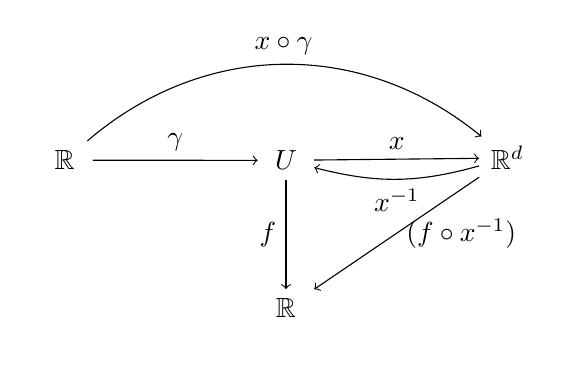
\begin{tikzpicture}[decoration=snake]
  \matrix (m) [matrix of math nodes, row sep=4em, column sep=6em, minimum width=2em]
  {
 \mathbb{R} & U & \mathbb{R}^d \\
& \mathbb{R} &  \\
};
  \path[->]
  (m-1-1) edge node [above] {$\gamma$} (m-1-2)
          edge [bend left=40] node [auto] {$x\circ \gamma$} (m-1-3)
  (m-1-3) edge [bend left=15] node [auto] {$x^{-1}$} (m-1-2)
          edge node [right] {$(f\circ x^{-1})$ } (m-2-2)
  (m-1-2) edge node [left] {$f$} (m-2-2)
          edge node [auto] {$x$} (m-1-3);
\end{tikzpicture} \quad \quad \, 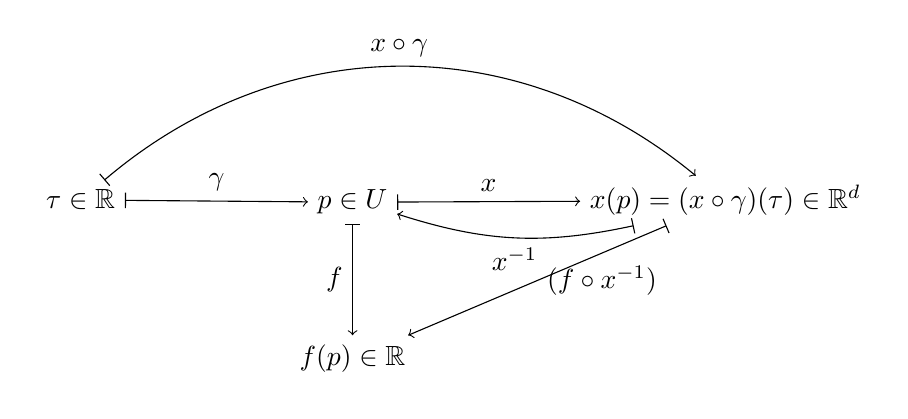
\begin{tikzpicture}[decoration=snake]
  \matrix (m) [matrix of math nodes, row sep=4em, column sep=6em, minimum width=2em]
  {
 \tau \in \mathbb{R} & p \in U & x(p) = (x\circ \gamma)(\tau) \in \mathbb{R}^d \\
& f(p) \in \mathbb{R} &  \\
};
  \path[|->]
  (m-1-1) edge node [above] {$\gamma$} (m-1-2)
          edge [bend left=40] node [auto] {$x\circ \gamma$} (m-1-3)
  (m-1-3) edge [bend left=15] node [auto] {$x^{-1}$} (m-1-2)
          edge node [right] {$(f\circ x^{-1})$ } (m-2-2)
  (m-1-2) edge node [left] {$f$} (m-2-2)
          edge node [auto] {$x$} (m-1-3);
\end{tikzpicture}



\questionhead{:} Consider, for $d=2$,
\[
(x\circ \gamma)(\lambda):= (\cos{(\lambda)}, \sin{(\lambda)} ) \text{ and } (f\circ x^{-1})((x,y)) := x^2 +y^2
\]
Using the chain rule, calculate
\[
(f\circ \gamma)'(\lambda)
\]
explicitly.

\solutionhead{:}

EY : 20151109 Indeed, the domains and codomains of this $f\gamma$ mapping makes sense, from $\mathbb{R} \to \mathbb{R}$ for 
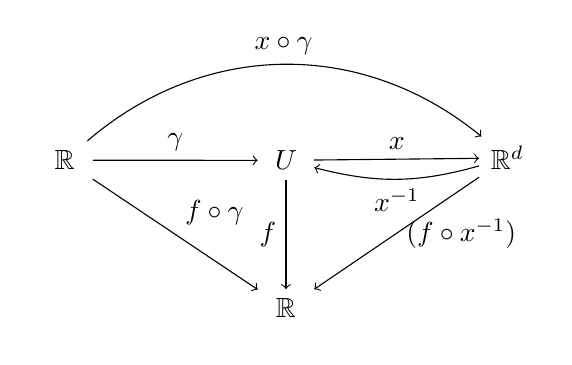
\begin{tikzpicture}[decoration=snake]
  \matrix (m) [matrix of math nodes, row sep=4em, column sep=6em, minimum width=2em]
  {
 \mathbb{R} & U & \mathbb{R}^d \\
& \mathbb{R} &  \\
};
  \path[->]
  (m-1-1) edge node [above] {$\gamma$} (m-1-2)
          edge [bend left=40] node [auto] {$x\circ \gamma$} (m-1-3)
          edge node [auto] {$f\circ \gamma$} (m-2-2)
  (m-1-3) edge [bend left=15] node [auto] {$x^{-1}$} (m-1-2)
          edge node [right] {$(f\circ x^{-1})$ } (m-2-2)
  (m-1-2) edge node [left] {$f$} (m-2-2)
          edge node [auto] {$x$} (m-1-3);
\end{tikzpicture} \quad \quad \, 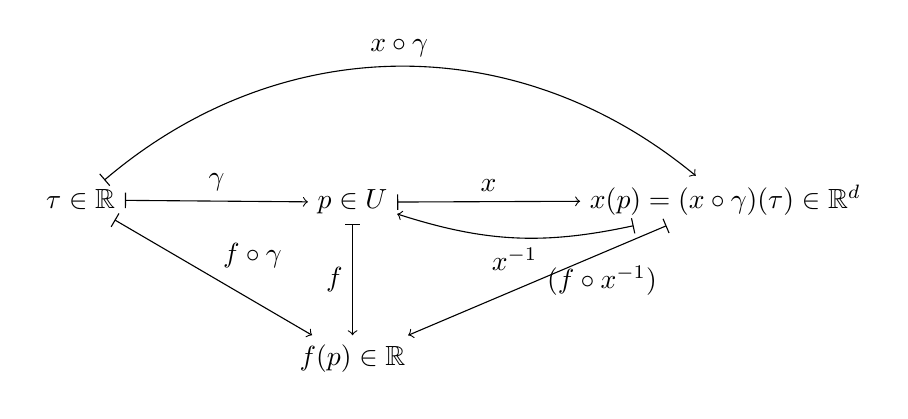
\begin{tikzpicture}[decoration=snake]
  \matrix (m) [matrix of math nodes, row sep=4em, column sep=6em, minimum width=2em]
  {
 \tau \in \mathbb{R} & p \in U & x(p) = (x\circ \gamma)(\tau) \in \mathbb{R}^d \\
& f(p) \in \mathbb{R} &  \\
};
  \path[|->]
  (m-1-1) edge node [above] {$\gamma$} (m-1-2)
          edge [bend left=40] node [auto] {$x\circ \gamma$} (m-1-3)
          edge node [auto] {$f\circ \gamma$} (m-2-2)
  (m-1-3) edge [bend left=15] node [auto] {$x^{-1}$} (m-1-2)
          edge node [right] {$(f\circ x^{-1})$ } (m-2-2)
  (m-1-2) edge node [left] {$f$} (m-2-2)
          edge node [auto] {$x$} (m-1-3);
\end{tikzpicture}

\[
\begin{gathered}
  (f\circ \gamma)'(\lambda) = (Df)\cdot \dot{\gamma}(\lambda) = \frac{ \partial f}{ \partial x^j} \dot{\gamma}^j(\lambda) = 2x (-\sin{\lambda} ) + 2y \cos{\lambda} = 2(-\cos{\lambda} \sin{\lambda} + \sin{\lambda} \cos{\lambda} ) = 0 
\end{gathered}
\]


\section{Lecture 8: Parallel Transport \& Curvature}

\subsection{Parallelity of vector fields}

\begin{definition}
\begin{enumerate}
\item[(1)]  \textbf{parallely transported} along smooth curve $\gamma: \mathbb{R} \to M$  

if 
\begin{equation}
  \boxed{ \nabla_{ v_{\gamma} } X = 0 }
\end{equation}
\item[(2)] A slightly weaker condition 

is ``parallel''

\[
( \nabla_{v_{\gamma, \gamma(\lambda)} } X)_{\gamma(\lambda)} = \mu(\lambda) X_{\gamma(\lambda)}
\]


\end{enumerate}
\end{definition}

\subsection{Autoparallely transported curves}

\begin{definition}
curve $\gamma: \mathbb{R} \to M$ is called \\
\textbf{autoparallely transported} if 
\begin{equation}
  \nabla_{v_{\gamma}}v_{\gamma} \overset{!}{=} 0
\end{equation}
\end{definition}


\subsection{Autoparallel equation}

\[
\nabla_{v_{\gamma}} v_{\gamma} =0 
\]

in summary:
\begin{equation}
  \ddot{\gamma}^m_{(x)}(\lambda) + (\Gamma^m_{(x)})_{ab}(\gamma(\lambda)) \dot{\gamma}^a_{(x)}(\lambda) \dot{\gamma}^b_{(x)}(\lambda) = 0 
\end{equation}

\subsection{Torsion}

\begin{definition}
  \textbf{torsion} of a connection $\nabla$ is the $(1,2)$-\textbf{tensor field}
\begin{equation}
  T(\omega,X,Y) := \omega( \nabla_X Y - \nabla_Y X - [X,Y])
\end{equation}
\end{definition}

(Inside a cloud) 

$[X,Y]$ vector field defined by 
\[
[X,Y]f:= X(Yf) - Y(Xf)
\]

\begin{proof}
  check $T$ is $C^{\infty}$-linear in each entry

\[
\begin{gathered}
  T(\omega, fX,Y) = \omega ( \nabla_{fX} Y - \nabla_Y (fX) - [fX,Y] )
\end{gathered}
\]
\end{proof}

\begin{definition}
  A $(M, \mathcal{O}, \mathcal{A}, \nabla)$ is called torsion-free if $T=0$
\end{definition}

In a chart 
\[
\begin{aligned}
  T^i_{ \, \, ab } := T\left(dx^i , \frac{ \partial }{ \partial x^a} , \frac{ \partial }{ \partial x^b}  \right) & = dx^i ( \dots ) \\ 
  & = \Gamma^i_{ \, \, ab} - \Gamma^i_{ \, \, ba} = 2 \Gamma^i_{ \, \, [ab] }
\end{aligned}
\]

From now on, in these lectures, we only use torsion-free connections. 

\subsection{Curvature}

\begin{definition}
  \textbf{Riemann curvature} of a connection $\nabla$ is the $(1,3)$-tensor field
\begin{equation}
  \text{Riem}(\omega,Z,X,Y) := \omega( \nabla_X \nabla_Y Z - \nabla_Y \nabla_X Z - \nabla_{[X,Y]} Z)
\end{equation}
\end{definition}
\begin{proof}
  do it: $C^{\infty}$-linear in each slot.  
\end{proof}

\underline{Tutorials} $\text{Riem}^i_{ \,\, jab} = \dots $
 % Parallel Transport & Curvature
%\section*{Tutorial 8 Parallel transport \& Curvature}

\exercisehead{1}

\exercisehead{2}\textbf{: Where connection coefficients appear}

It was suggested in the tutorial sheets and hinted in the lecture that the following should be committed to memory.

\questionhead{: Recall the autoparallel equation for a curve $\gamma$}
\begin{enumerate}
\item[(a)] \[
\nabla_{v_{\gamma}} v_{\gamma} = 0 
\]
\item[(b)]
\[
\nabla_{v_{\gamma}} v_{\gamma} = \nabla_{ \dot{\gamma} \frac{ \partial }{ \partial x^{\mu}} } v_{\gamma} = \dot{\gamma}^{\nu} \nabla_{ \partial_{\nu}} v_{\gamma} = \dot{\gamma}^{\nu} \left[ \frac{ \partial v^{\mu}_{\gamma}}{ \partial x^{\nu} } + \Gamma^{\rho}_{\mu \nu} v_{\gamma}^{\mu} \right] \frac{ \partial }{ \partial x^{\rho }} = \dot{\gamma}^{\nu} \left[ \frac{ \partial \dot{\gamma}^{\rho }}{ \partial x^{\nu}} + \Gamma^{\rho}_{\mu \nu} \dot{\gamma}^{\mu} \right] \frac{ \partial }{ \partial x^{\rho }} = 0
\]
\[
\Longrightarrow \boxed{ \ddot{\gamma}^{\rho} + \Gamma^{\rho}_{\mu \nu} \dot{\gamma}^{\mu} \dot{\gamma}^{\nu} }
\]
as, for example, for $F(x(t))$, 
\[
\frac{dF(x(t))}{dt} = \dot{x} \frac{ \partial F}{ \partial x} = \frac{d}{dt} F
\]
so that 
\[
\dot{\gamma}^{\nu} \frac{ \partial v_{\gamma}^{\mu} }{ \partial x^{\nu}} = \frac{d}{d\lambda} v_{\gamma}^{\mu} = \frac{d^2}{d\lambda^2} \gamma^{\mu}
\]
\end{enumerate}

\questionhead{: Determine the coefficients of the Riemann tensor with respect to a chart $(U,x)$}

Recall this manifestly covariant definition

\[
\text{Riem}(\omega, Z,X,Y) = \omega ( \nabla_X \nabla_Y Z - \nabla_Y \nabla_X Z - \nabla_{[X,Y]}Z )
\]
We want $R^i_{ \, \, jab}$.  

now
\[
\begin{gathered}
  \nabla_X \nabla_Y Z = \nabla_X ( ( Y^{\mu} \frac{ \partial }{ \partial x^{\mu }} Z^{\rho} + \Gamma^{\rho}_{\mu \nu } Z^{\mu} Y^{\nu} ) \frac{\partial}{ \partial x^{\rho}} ) = (X^{\alpha} \frac{ \partial }{ \partial x^{\alpha}} (Y^{\mu} \frac{ \partial }{ \partial x^{\mu}} Z^{\rho} + \Gamma^{\rho}_{ \mu \nu} Z^{\mu} Y^{\nu}  ) + \Gamma^{\rho}_{\alpha \beta} (Y^{\mu} \frac{ \partial }{ \partial x^{\mu} } Z^{\alpha} + \Gamma^{\alpha}_{\mu \nu} Z^{\mu} Y^{\nu} ) X^{\beta} )\frac{\partial }{ \partial x^{\rho }}
\end{gathered}
\]

For $X = \partial_a$, $Y = \partial_b$, $Z=\partial_j$, then the partial derivatives of the coefficients of the input vectors become zero.  

\[
\Longrightarrow \nabla_{ \partial_a} \nabla_{\partial_b} \partial_j = \frac{ \partial }{ \partial x^a} (\Gamma^i_{ jb} ) + \Gamma^i_{\alpha a} \Gamma^{\alpha}_{jb}
\]

Now
\[
[X,Y]^i = X^j \frac{ \partial }{ \partial x^j} Y^i - Y^j \frac{ \partial X^i}{ \partial x^j}
\]
For coordinate vectors, $[\partial_i, \partial_j] = 0$ $\forall \, i,j = 0, 1 \dots d$.  

Thus
\[
\boxed{ R^i_{ \, \, jab} = \frac{ \partial }{ \partial x^a} \Gamma^i_{jb} - \frac{ \partial }{ \partial x^b} \Gamma^i_{ja} + \Gamma^i_{\alpha a} \Gamma^{\alpha}_{jb} -\Gamma^i_{\alpha b} \Gamma^{\alpha}_{ja} }
\]


\questionhead{:$\text{Ric}(X,Y):=\text{Riem}^m_{ \, \, amb} X^a Y^b$ define $(0,2)$-tensor?}

Yes, transforms as such:

\[
\begin{gathered}
  \end{gathered}
\]

\subsection*{EY developments}

I roughly follow the spirit in Theodore Frankel's \textbf{The Geometry of Physics: An Introduction} Second Ed. 2003, Chapter 9 Covariant Differentiation and Curvature, Section 9.3b. The Covariant Differential of a Vector Field. P.S. EY : 20150320 I would like a copy of the Third Edition but I don't have the funds right now to purchase the third edition: go to my tilt crowdfunding campaign, \url{http://ernestyalumni.tilt.com}, and help with your financial support if you can or send me a message on my various channels and ernestyalumni gmail email address if you could help me get a hold of a digital or hard copy as a pro bono gift from the publisher or author.  

The spirit of the development is the following:
\begin{quote}
``How can we express connections and curvatures in terms of forms?'' -Theodore Frankel.  
\end{quote}

From Lecture 7, connection $\nabla$ on vector field $Y$, in the ``direction'' $X$,
\[
\begin{gathered}
  \nabla_{ \frac{ \partial }{ \partial x^k } } Y = \left( \frac{ \partial Y^i }{ \partial x^k } + \Gamma^i_{jk} Y^j  \right) \frac{ \partial }{ \partial x^i }
\end{gathered}
\]
Make the ansatz (approche, impostazione) that the connection $\nabla$ acts on $Y$, the vector field, first:
\[
\begin{gathered}
  \nabla Y(X) = \left( X^k \frac{ \partial Y^i}{ \partial x^k} + \Gamma^i_{jk} Y^j X^k \right) \frac{ \partial}{ \partial x^i } = X^k \left( \nabla_{ \frac{ \partial }{ \partial x^k} } Y \right)^i \frac{ \partial }{ \partial x^i} = (\nabla_X Y)^i \frac{ \partial}{ \partial x^i} = \nabla_XY
\end{gathered}
\]

Now from Lecture 7, Definition for $\Gamma$, 
\[
dx^i \left( \nabla_{ \frac{  \partial }{ \partial x^k } } \frac{ \partial }{ \partial x^j } \right) = \Gamma^i_{jk}
\]

Make this ansatz (approche, impostazine)
\[
\nabla \frac{ \partial}{ \partial x^j } = \left( \Gamma^i_{jk} dx^k \right) \otimes \frac{ \partial }{ \partial x^i} \in \Omega^1(M,TM) = T^*M \otimes TM
\]
where $\Omega^1(M,TM) = T^*M \otimes TM$ is the set of all $TM$ or vector-valued 1-forms on $M$, with the 1-form being the following:
\[
\Gamma^i_{jk} dx^k = \Gamma^i_{ \, \, j } \in \Omega^1(M) \quad \quad \, \begin{aligned}
  & \quad \\
  & i = 1 \dots \text{dim}(M) \\ 
  & j = 1\dots \text{dim}(M) \end{aligned}
\]
So $\Gamma^i_{ \, \, j}$ is a $\text{dim}M \times \text{dim}M$ matrix of 1-forms (EY !!!). 

Thus
\[
\nabla Y = (d(Y^i) + \Gamma^i_j Y^j ) \otimes \frac{ \partial }{ \partial x^i}
\]

So the connection is a (smooth) map from $TM$ to the set of all vector-valued 1-forms on $M$, $\Omega^1(M,TM)$, and then, after ``eating'' a vector $Y$, yields the ``covariant derivative'':
\[
\begin{aligned}
  & \nabla: TM \to \Omega^1(M,TM) = T^*M \otimes TM \\ 
  & \nabla : Y \mapsto \nabla Y \\ 
  & \nabla Y : TM \to TM \\
  & \nabla Y(X) \mapsto \nabla Y(X) = \nabla_X(Y)
\end{aligned}
\]

Now
\[
\left[ \frac{ \partial }{ \partial x^i} , \frac{ \partial }{ \partial x^j} \right] f = \frac{ \partial }{ \partial x^i } \left( \frac{ \partial }{ \partial x^j} \right) - \frac{ \partial }{ \partial x^j } \left( \frac{ \partial }{ \partial x^i} \right) = 0 
\]
(this is okay as on $p \in (U,x)$; $x$-coordinates on same chart $(U,x)$)

EY : 20150320 My question is when is this nontrivial or nonvanishing (i.e. not equal to $0$).
\[
[e_a,e_b] = ?
\]
for a frame $(e_c)$ and would this be the difference between a tangent bundle $TM$ vs. a (general) vector bundle?

Wikipedia helps here. cf. wikipedia, ``Connection (vector bundle)''

\[
\begin{gathered}
  \nabla : \Gamma(E) \to \Gamma(T^*M \otimes E) = \Omega^1(M,E) \\
  \nabla e_a = \omega^c_{ab} f^b \otimes e_c \\ 
  f^b \in T^*M \text{ (this is the dual basis for $TM$ and, note, this is for the manifold, $M$ } \\
  \nabla_{f_b}e_a = \omega^c_{ab} e_c \in E
\end{gathered}
\]
\[
\omega^c_a  = \omega^c_{ab} f^b \in \Omega^1(M)
\]
is the connection 1-form, with $a,c = 1 \dots \text{dim}V$.  EY : 20150320 This $V$ is a vector space living on each of the fibers of $E$.   I know that $\Gamma(T^*M \otimes E)$ looks like it should take values in $E$, but it's meaning that it takes vector values of $V$.  Correct me if I'm wrong: ernestyalumni at gmail and various social media.

Let $\sigma \in \Gamma(E)$, $\sigma = \sigma^ae_a$  
\[
\begin{gathered}
  \nabla \sigma = (d\sigma^c + \omega^c_{ab} \sigma^a f^b) \otimes e_c \text{ with } \\ 
  d\sigma^c = \frac{ \partial \sigma^c}{ \partial x^b } f^b 
\end{gathered}
\]
\[
\Longrightarrow \nabla_X \sigma = \left( X^b \frac{ \partial \sigma^c}{ \partial x^b} + \omega^c_{ab} \sigma^a X^b \right)e_c = X^b \left( \frac{ \partial \sigma^c}{ \partial x^b } + \omega^c_{ab} \sigma^a \right)e_c
\]


\section{Lecture 9: Newtonian spacetime is curved!}

\begin{axiom}[Newton I:]
  A body on which \emph{no} force acts moves uniformly along a straight line 
\end{axiom}

\begin{axiom}[Newton II:]
Deviation of a body's motion from such uniform straight motion is effected by a force, reduced by a factor of the body's reciprocal mass.  
\end{axiom}

\underline{Remark}: \begin{enumerate}
\item[(1)] 1st axiom - in order to be relevant - must be read as a measurement prescription for the geometry of space $\dots $
\item[(2)] Since gravity universally acts on every particle, in a universe with at least two particles, gravity must not be considered a force if Newton I is supposed to remain applicable.  
\end{enumerate}

\subsection{Laplace's questions} Laplace $\begin{aligned}  & \quad \\ 
  & * 1749 \\
  & \dag 1827  \end{aligned}$

Q: ``Can gravity be encoded in a curvature of space, such that its effects show if particles under the influence of (no other) force we postulated to more along straight lines in this curved space?''

\underline{Answer}: No!

\begin{proof}
gravity is a force point of view


\[
m \ddot{x}^{\alpha}(t) = F^{\alpha}(x(t))
\]
\[
m\ddot{x}^{\alpha}(t) = \underbrace{mf^{\alpha}}_{F^{\alpha}}(x(t))
\]
$-\partial_{\alpha} f^{\alpha} = 4\pi G\rho$ (Poisson) \\
$\rho $ mass density of matter

(EY : 20150330) You know this, $F=Gm_1m_2/r^2$

\[
\ddot{x}^{\alpha}(t) - f^{\alpha}(x(t)) = 0 
\]
Laplace asks: Is this ($\ddot{x}(t)$) of the form 

\[
\ddot{x}^{\alpha}(t) + \Gamma^{\alpha}_{\, \, \beta \gamma}(x(t)) \dot{x}^{\beta}(t) \dot{x}^{\gamma}(t) = 0 
\]

Conclusion: One cannot find $\Gamma$ s such that Newton's equation takes the form of an autoparallel.

\end{proof}

\subsection{The full wisdom of Newton I}

use also the information from Newton's first law that particles (no force) move uniformly 

introduce the appropriate setting to talk about the difference easily

insight: in \underline{spacetime} $\boxed{ \text{ uniform \& straight motion }}$ is simply straight motion

So let's try in \underline{spacetime}: 

let $x: \mathbb{R} \to \mathbb{R}^3$ \\
\phantom{\quad } be a particle's trajectory in space $\longleftrightarrow $ worldline (history) of the particle $\begin{aligned} & \quad \\
  & X : \mathbb{R} \to \mathbb{R}^4  \\
  & t\mapsto (t, x^1(t), x^2(t),x^3(t)) := \\
  & := (X^0(t), X^1(t),X^2(t),X^3(t)) \end{aligned}$

That's all it takes:

Trivial rewritings:

\[
\dot{X}^0 =1
\]

\[
\Longrightarrow \boxed{ \begin{aligned}
  & \ddot{X}^0 & = 0 \\ 
  & \ddot{X}^{\alpha} - f^{\alpha}(X(t))\cdot \dot{X}^0 \cdot \dot{X}^0 & =0 
\end{aligned} } \quad \, (\alpha = 1,2,3)  \Longrightarrow \begin{gathered}
  a = 0,1,2,3 \\
  \boxed{ \ddot{X}^a + \Gamma^a_{ \, \, bc}\dot{X}^b \dot{X}^c = 0 } \\
  \text{ antoparallel eqn in \underline{spacetime } }
\end{gathered}
\]

Yes, choosing $\begin{aligned} & \quad \\
  & \Gamma^0_{ \, \, ab} = 0 \\
  & \Gamma^{\alpha}_{ \, \, \beta \gamma} = 0 =Gamma^{\alpha}_{\,\, 0\beta} = \Gamma^{\alpha}_{ \, \, \beta 0}\end{aligned}$

\underline{only}: $\boxed{ \Gamma^{\alpha}_{ \, \, 00} \overset{!}{=} -f^{\alpha}}$

\underline{Question}: Is this a coordinate-choice artifact?

No, since $R^{\alpha}_{ \, \, 0\beta 0} = - \frac{ \partial }{ \partial x^{\beta}} f^{\alpha}$ (only non-vanishing components) (tidal force tensor, $-$ the Hessian of the force component)

Ricci tensor $\Longrightarrow  R_{00} = R^m_{ \, \, 0m0} = -\partial_{\alpha} f^{\alpha} = 4\pi G \rho$
 
Poisson: $-\partial_{\alpha}f^{\alpha} = 4\pi G\cdot \rho$

\underline{writing}: $T_{00} = \frac{1}{2}s$ 
\[
\Longrightarrow \boxed{ R_{00} = 8 \pi G T_{00} }
\]
Einstein in 1912 $ \boxed{ \xcancel{ R_{ab} = 8\pi G T_{ab} }}$


\underline{Conclusion}: Laplace's idea works in spacetime

\underline{Remark} 
\[
\begin{gathered}
  \Gamma^{\alpha}_{ \, \, 00 } = -f^{\alpha} \\ 
  R^{\alpha}_{ \, \, \beta \gamma \delta } = 0 \quad \quad \, \alpha, \beta , \gamma, \delta = 1,2,3 \\
  \boxed{ R_{00} = 4\pi G \rho }
\end{gathered}
\]

\underline{Q}: What about transformation behavior of LHS of 
\[
\underbrace{ \ddot{x}^a + \Gamma^a_{ \, \, bc } \dot{X}^b \dot{X}^c}_{ \underbrace{ (\nabla_{v_X}v_X)^a}_{ := a^a \text{ ``acceleration \underline{vector}'' } } } = 0
\]

\subsection{The foundations of the geometric formulation of Newton's axiom}

new start
\begin{definition}
A \textbf{Newtonian spacetime} is a quintuple \[
(M , \mathcal{O}, \mathcal{A}, \nabla , t)
\]
where $(M,\mathcal{O}, \mathcal{A})$ 4-dim. smooth manifold
\[
t: M \to \mathbb{R} \text{ smooth function }
\]

\begin{enumerate}
  \item[(i)] ``There is an absolute space''
\[
(dt)_p \neq 0 \quad \quad \, \forall \, p \in M 
\]
    \item[(ii)] ``absolute time flows uniformly''
\[
\nabla dt \underbrace{=}_{ \text{ space of $(0,2)$-tensor fields } }  0 \quad \quad \, \text{ everywhere }
\]
$\nabla dt $ is a $(0,2)$-tensor field
\item[(iii)] add to axioms of Newtonian spacetime 
$\nabla = 0$ torsion free
\end{enumerate}
\end{definition}

\begin{definition}
  absolute space at time $\tau$ 
\[
S_{\tau} := \lbrace p\in M | t(p) = \tau \rbrace
\]
\[
\xrightarrow{ dt \neq 0 } M = \coprod S_{\tau}
\]
\end{definition}

\begin{definition} A vector $X \in T_p M$ is called 
\begin{enumerate}
\item[(a)] future-directed if 
\[
dt(X) > 0 
\]
\item[(b)] spatial if 
\[
dt(X) = 0 
\]
\item[(c)]
past-directed if 
\[
dt(X) < 0
\]
\end{enumerate}
\end{definition}

\underline{picture}

\underline{Newton I}: The worldline of a particle under the influence of no force (gravity isn't one, anyway) is a \underline{future-directed autoparallel } i.e.

\[
\begin{gathered}
  \nabla_{v_{X}} v_{X} = 0 \\
  dt(v_{X}) > 0 
\end{gathered}
\]

\underline{Newton II}: 
\[
\nabla_{v_{X}} v_X = \frac{F}{m} \Longleftrightarrow m \cdot a = F
\]


where $F$ is a spatial vector field:
\[
dt(F) = 0 
\]

\textbf{Convention}: restrict attention to atlases $\mathcal{A}_{\text{stratefied}}$ whose charts $(\mathcal{U}, x)$ have the property

\[
\begin{aligned}
  & x^0:\mathcal{U} \to \mathbb{R} \\ 
  & x^1: \mathcal{U} \to \mathbb{R} \\ 
  & \vdots \quad \, \vdots \\ 
  & x^3
\end{aligned}
\quad \quad \, 
x^0 = \left. t \right|_{\mathcal{U}}  \quad\quad \, \Longrightarrow \begin{gathered} 0 \overset{\text{``absolute time flows uniformly''} }{=} \nabla dt \\
0 = \nabla_{\frac{ \partial }{ \partial x^a} } dx^0 = - \Gamma_{ \, \, ba }^0 \quad \quad \, a = 0,1,2,3
\end{gathered}
\]

Let's evaluate in a chart $(\mathcal{U},x)$ of a stratified atlas $\mathcal{A}_{\text{sheet}}$: Newton II:

\[
\nabla_{v_X} v_X = \frac{F}{m}
\]
in a chart.
\[
\begin{aligned}
& (X^0)'' + \cancel{ \Gamma^0_{ \, \, cd } (X^a)' (X^b)' }^{ \text{stratified atlas}} = 0  \\
  & (X^{\alpha})'' + \Gamma^{\alpha}_{\gamma \delta} X^{\gamma'} X^{\delta'} + \Gamma^{\alpha}_{ \, \, 00} X^{0'} X^{0'} + 2\Gamma^{\alpha}_{ \, \, \gamma 0} X^{\gamma'} X^{0'} = \frac{F^{\alpha}}{m} \quad \quad \, \alpha = 1,2,3
\end{aligned}
\]

\[
\begin{gathered}
\Longrightarrow (X^0)''(\lambda) = 0 \Longrightarrow X^0(\lambda) = a\lambda + b \quad \, \text{ constants $a,b$ } \text{ with  }  \\
X^0(\lambda) = (x^0 \circ X)(\lambda) \overset{\text{stratified}}{=} (t\circ X)(\lambda)
\end{gathered}
\]
\underline{convention} parametrize worldline by absolute time

\[
\frac{d}{d\lambda} = a \frac{d}{dt}
\]
\[
\begin{gathered}
a^2 \ddot{X}^{\alpha} + a^2 \Gamma^{\alpha}_{ \, \, \gamma \delta} \dot{X}^{\gamma} \dot{X}^{\delta} + a^2 \Gamma^{\alpha}_{ \, \, 00 } \dot{X}^0 \dot{X}^0 + 2\Gamma^{\alpha}_{ \, \,\gamma 0} \dot{X}^{\gamma} \dot{X}^{0} =  \frac{ F^{\alpha}}{ m} \\
\Longrightarrow  \underbrace{ \ddot{X}^{\alpha} +  \Gamma^{\alpha}_{ \, \, \gamma \delta} \dot{X}^{\gamma} \dot{X}^{\delta} +  \Gamma^{\alpha}_{ \, \, 00 } \dot{X}^0 \dot{X}^0 + 2\Gamma^{\alpha}_{ \, \,\gamma 0} \dot{X}^{\gamma} \dot{X}^{0} }_{a^{\alpha} } = \frac{1}{a^2} \frac{ F^{\alpha}}{ m} 
\end{gathered}
\]
 % Newtonian spacetime is curved!

\section{Metric Manifolds}
We establish a structure on a smooth manifold that allows one to assign vectors in each tangent space a length (and an angle between vectors in the same tangent space).

From this structure, one can then define a notion of length of a curve. \\
Then we can look at shortest curves.

Requiring then that the shortest curves coincide with the straightest curves (wrt $\nabla$) will result in $\nabla$ being determined by the metric structure.  
\[
g  \overset{\substack{\text{straight} = \text{short} \\ T =0 }}{\rightsquigarrow}  \nabla \rightsquigarrow Riem
\]

\subsection{Metrics}
\begin{definition}
  A metric $g$ on a smooth manifold $(M,\mathcal{O}, \mathcal{A})$ is a $(0,2)$-tensor field satisfying
\begin{enumerate}
\item[(i)] \textbf{symmetry:} $g(X,Y) = g(Y,X) \quad \forall \, X, Y \text{vector fields}$
\item[(ii)] \underline{non-degeneracy}: the \underline{musical map}
\[
\begin{aligned}
  \text{``flat''} \, \,  \flat : \Gamma(TM) & \to \Gamma(T^*M) \\ 
  X \mapsto \flat(X)
\end{aligned}
\]
\emph{where} \quad \,  $\begin{aligned} & \quad \quad \\ 
  & \flat(X)(Y):= g(X,Y) \\
  & \flat(X) \in \Gamma(T^*M) \end{aligned}$ \\
In thought bubble: $\flat(X) = g(X,\cdot)$

\dots is a $C^{\infty}$-isomorphism in other words, it is invertible.
\end{enumerate}
\end{definition}

\underline{Remark}: $(\flat(X))_a$ \quad \, or \\
$X_a$ \\
$(\flat(X))_a := g_{am} X^m$

Thought bubble: $\flat^{-1} = \sharp$

$\flat^{-1}(\omega)^a := g^{am}\omega_m$ \\
$\flat^{-1}(\omega)^a := (g^{``-1''})^{am}\omega_m$
$\Longrightarrow $ not needed.  (all of this is not needed)

\begin{definition}
  The $(2,0)$-tensor field $g^{``-1''}$ with respect to a metric $g$ is the symmetric
\[
\begin{aligned}
  g^{``-1''} : \Gamma(T^*M) \times \Gamma(T^*M) \xrightarrow{ ~ } C^{\infty}(M) \\
  (\omega, \sigma) \mapsto \omega( \flat^{-1}(\sigma)) \quad \quad \, \flat^{-1}(\sigma) \in \Gamma(TM))
\end{aligned}
\]

\underline{chart}:
\begin{align*}
g_{ab} = g_{ba} & \quad \quad (g^{-1})^{am} g_{mb} = \delta^a_b
\end{align*}
\end{definition}

\underline{Example}: Consider $(S^2, \mathcal{O}, \mathcal{A})$ and the chart $(U,x)$
\begin{align*}
\varphi \in (0,2\pi), & \quad \quad \theta \in (0,\pi)
\end{align*}

Define the metric \\
\[
g_{ij}(x^{-1}(\theta,\varphi)) = \left[ \begin{matrix} R^2 & 0 \\
    0 & R^2\sin^2{\theta} \end{matrix} \right]_{ij}
\]
$R \in \mathbb{R}^+$

``the metric of the \underline{round sphere of radius $R$}''

\subsection{Signature}
Linear algebra: \quad \quad \, $\begin{aligned} & A\indices{^a_{m}}v^m = \lambda v^a & \quad \quad \quad \, \left(\begin{matrix} \lambda_1 & & 0 \\
    & \ddots & \\ 
    0 & & \lambda_n \end{matrix} \right) \\
  & g_{am} v^m = \lambda \cdot v^a ? \rightsquigarrow  & \quad \quad \quad \, \left( \begin{matrix} 
    1        &   &    &        &    &   &        & \\
    & \ddots &   &    &        &    &   &        & \\
    &        & 1 &    &        &    &   &        & \\
    &        &   & -1 &        &    &   &        & \\
    &        &   &    & \ddots &    &   &        & \\
    &        &   &    &        & -1 &   &        & \\
    &        &   &    &        &    & 0 &        & \\
    &        &   &    &        &    &   & \ddots & \\
    &        &   &    &        &    &   &        & 0 \end{matrix} \right)
\end{aligned}$

$(1,1)$ tensor has eigenvalues \\
$(0,2)$ has \underline{signature} $(p,q)$ (well-defined)

$\left. \begin{aligned}
  (+++) \\
  (++-) \\
  (+--) \\
  (---) \end{aligned} \right\rbrace$ $d+1$ if $p+q = \text{dim}V$

\begin{definition} A metric is called \textbf{Riemannian} if its signature is $(++ \dots +)$, and \textbf{Lorentzian} if it is $(+-\dots -)$.
\end{definition}

\subsection{Length of a curve}
Let $\gamma$ be a smooth curve. Then we know its veloctiy $v_{\gamma,\gamma(\lambda)}$ at each $\gamma(\lambda) \in M$.

\begin{definition}
On a Riemannian metric manifold $(M, \mathcal{O}, \mathcal{A}, g)$, the \textbf{speed} of a curve at $\gamma(\lambda)$ is the number 
\begin{equation}
\boxed{s(\lambda) = (\sqrt{g(v_{\gamma}, v_{\gamma})})_{\gamma(\lambda)}}
\end{equation}
\end{definition}

(I feel the need for speed, then I feel the need for a metric)

\underline{Aside}: $[v^a] = \frac{1}{T}$ \\
\phantom{Aside:} $[g_{ab}] = L^2 $ \\
\phantom{Aside:} $[\sqrt{g_{ab}v^av^b}] = \sqrt{ \frac{L^2}{T^2}} = \frac{L}{T}$

\begin{definition}
Let $\gamma:(0,1) \to M$ a smooth curve. Then the \textbf{length of $\gamma$}, $L[\gamma] \in \mathbb{R}$ is the number
\begin{equation}
\boxed{L[\gamma] := \int_0^1 d\lambda s(\lambda) = \int_0^1 d\lambda \sqrt{ (g(v_{\gamma}, v_{\gamma}))_{\gamma(\lambda)}}}
\end{equation}
\end{definition}

F. Schuller: ``velocity is more fundamental than speed, speed is more fundamental than length''

\textbf{Example:} Reconsider the round sphere of radius $R$. Consider its equator:
\begin{align*}
\theta(\lambda) := (x^1 \after \gamma)(\lambda) = \frac{\pi}{2}, & \quad \varphi(\lambda) := (x^2 \after \gamma)(\lambda) = 2\pi \lambda^3 \\
\implies \theta'(\lambda) = 0, & \quad \varphi'(\lambda) = 6\pi\lambda^2
\end{align*}

On the same chart $g_{ij} = \left[ \begin{matrix} R^2 & \\
    & R^2 \sin^2{\theta} \end{matrix} \right]$

Do everything in this chart
\begin{align*}
L[\gamma] & = \int_0^1 d\lambda \sqrt{g_{ij}(x^{-1}(\theta(\lambda), \varphi(\lambda)))(x^i \after \gamma)'(\lambda)(x^j \after \gamma)'(\lambda)} \\
& = \int_0^1 d\lambda \sqrt{R^2 \cdot 0 + R^2\sin^2{(\theta(\lambda))} 36 \pi^2 \lambda^4} \\
& = 6\pi R \int_0^1 d\lambda \lambda^2 = 6\pi R [\frac{1}{3} \lambda^3]^1_0 = 2\pi R
\end{align*}

\begin{theorem}
$\gamma : (0,1) \to M$ and $\sigma :(0,1) \to (0,1)$ smooth bijective and \underline{increasing} ``reparametrization'' \\
$L[\gamma] = L[\gamma \after \sigma]$
\end{theorem}

\begin{proof}
  $\Longrightarrow $ Tutorials
\end{proof}

\subsection{Geodesics}
\begin{definition}
A curve $\gamma : (0,1) \to M$ is called a \textbf{geodesic} on a Riemannian manifold $(M, \mathcal{O}, \mathcal{A}, g)$ if it is a stationary curve with respect to a length functional $L$.
\end{definition}

Thought bubble: In classical mechanics, deform the curve a little, $\epsilon$ times this deformation, to first order, it agrees with $L[\gamma]$.

\begin{theorem}
$\gamma$ geodesic iff it satisfies the Euler-Lagrange equations for the Lagrangian
\end{theorem}

\begin{align*}
\mathcal{L} : & TM \to \mathbb{R} \\
& X \mapsto \sqrt{g(X,X)}
\end{align*}
In a chart, the Euler Lagrange equations take the form:
\[
\left(\cibasis[\mathcal{L}]{\dot{x}^m}\right)^{\cdot} - \cibasis[\mathcal{L}]{x^m} = 0 
\]
F.Schuller: this is a chart dependent formulation

here: 
\[
\mathcal{L}(\gamma^i, \dot{\gamma}^i) = \sqrt{g_{ij}(\gamma(\lambda)) \dot{\gamma}^i(\lambda) \dot{\gamma}^j(\lambda)}
\]

Euler-Lagrange equations:
\begin{align*}
\cibasis[\mathcal{L}]{\dot{\gamma}^m} = \frac{1}{\sqrt{\dots}} g_{mj}(\gamma(\lambda)) \dot{\gamma}^j(\lambda) \\
\left(\cibasis[\mathcal{L}]{\dot{\gamma}^m}\right)^{\cdot} = \left(\frac{1}{\sqrt{\dots}} \right)^{\cdot} g_{mj}(\gamma(\lambda)) \cdot \dot{\gamma}^j(\lambda) + \frac{1}{\sqrt{\dots}} \left(g_{mj}(\gamma(\lambda)) \ddot{\gamma}^j(\lambda) + \dot{\gamma}^s(\partial_s g_{mj}) \dot{\gamma}^j(\lambda) \right)
\end{align*}

Thought bubble: reparametrize $g(\dot{\gamma}, \dot{\gamma}) = 1$ (it's a condition on my reparametrization)

By a clever choice of reparametrization $(\frac{1}{\sqrt{\dots}})^{\cdot} = 0$
\[
\begin{gathered}
  \cibasis[\mathcal{L}]{\gamma^m} = \frac{1}{2\sqrt{\dots}} \partial_m g_{ij}(\gamma(\lambda)) \dot{\gamma}^i(\lambda) \dot{\gamma}^j(\lambda)
\end{gathered}
\]
putting this together as Euler-Lagrange equations:
\[
\begin{gathered}
g_{mj} \ddot{\gamma}^j + \partial_s g_{mj} \dot{\gamma}^s \dot{\gamma}^j - \frac{1}{2} \partial_m g_{ij} \dot{\gamma}^i \dot{\gamma}^j = 0
\end{gathered}
\]
Multiply on both sides $(g^{-1})^{qm}$
\[
\begin{gathered}
\ddot{\gamma^q} + (g^{-1})^{qm}(\partial_i g_{mj} - \frac{1}{2} \partial_m g_{ij}) \dot{\gamma}^i \dot{\gamma}^j = 0  \\
\boxed{\ddot{\gamma^q} + (g^{-1})^{qm}\frac{1}{2} (\partial_i g_{mj} + \partial_j g_{mi} - \partial_m g_{ij}) \dot{\gamma}^i \dot{\gamma}^j = 0}
\end{gathered}
\]
geodesic equation for $\gamma$ in a chart.  
\[
\boxed{(g^{-1})^{qm}\frac{1}{2} (\partial_i g_{mj} + \partial_j g_{mi} - \partial_m g_{ij} ) =: \ccf{q}{ij}(\gamma(\lambda))
}
\]

Thought bubble: $\left(\cibasis[\mathcal{L}]{\xi_x^{a+\text{dim}M}} \right)^{\cdot}_{\sigma(x)} - \left(\cibasis[\mathcal{L}]{xi^a_x} \right)_{\sigma(x)} = 0$

\begin{definition}
\textbf{Christoffel symbol} ${\,}^{\text{L.C.}}\Gamma$ are the connection coefficient functions of the so-called Levi-Civita connection ${\,}^{\text{L.C.}}\nabla$
\end{definition}
We usually make this choice of $\nabla$ if $g$ is given.  

$(M, \mathcal{O}, \mathcal{A}, g) \to (M, \mathcal{O}, \mathcal{A}, g, {\,}^{\text{L.C.}}\nabla)$

\underline{abstract way}: $\nabla g = 0$ and $T = 0$ (torsion) \\
$\Longrightarrow \nabla = {\,}^{\text{L.C.}}\nabla$

\begin{definition}
\begin{enumerate}[(a)]
\item The \textbf{Riemann-Christoffel curvature} is defined by 
\begin{equation}
\boxed{R_{abcd} := g_{am}R\indices{^m_{bcd}}}
\end{equation}

\item \textbf{Ricci}
\begin{equation}
\boxed{R_{ab} = R\indices{^m_{amb}}}
\end{equation}
Thought bubble: with a metric, ${\,}^{\text{L.C.}}\nabla$

\item (Ricci) scalar curvature:
\begin{equation}
\boxed{R = g^{ab} R_{ab}}
\end{equation}

Thought bubble: ${\,}^{\text{L.C.}}\nabla$
\end{enumerate}
\end{definition}

\begin{definition}
\textbf{Einstein curvature} of $(M, \mathcal{O}, \mathcal{A}, g)$ is defined as
\begin{equation}
\boxed{G_{ab} := R_{ab} - \frac{1}{2} g_{ab} R}
\end{equation}
\end{definition}

\underline{Convention}: $g^{ab} := (g^{``-1''})^{ab}$

F. Schuller: these indices are not being pulled up, because what would you pull them up with

(student) Question: Does the Einstein curvature yield new information? \\
Answer: \\
$g^{ab} G_{ab} = R_{ab} g^{ab} - \frac{1}{2} g_{ab} g^{ab} R = R - \delta^a_a R = R - \frac{1}{2} \text{dim}M \, R = (1- \frac{d}{2}) R$
 % Metric Manifolds
%\section*{Tutorial 9: Metric manifolds}



\exercisehead{3: Levi-Civita Connection}
Suppose torsion-free $T=0$ and metric-compatible connection $\nabla g=0$

\questionhead{Recall $T=0$ on a chart}






\[
\boxed{ \Gamma^c_{ba} = \frac{1}{2} (g^{-1})^{cm} \left( \frac{ \partial g_{bm} }{ \partial x^a} + \frac{ \partial g_{ma}}{ \partial x^b} - \frac{ \partial g_{ab}}{ \partial x^m} \right) }
\]
or 
\[
\Gamma^a_{bc} = \frac{1}{2} (g^{-1})^{am} \left( \frac{ \partial g_{bm}}{\partial x^c} + \frac{ \partial g_{mc}}{ \partial x^b} - \frac{ \partial g_{bc}}{ \partial x^m} \right)
\]




\section{Symmetry}
\begin{framed}
This lecture is about symmetry but we will pick a number of elementary techniques in differential geometry that we will need in Einstein's theory. We shall motivate these techniques by appealing to the feeling that the round sphere $(S^2, \mathcal{O}, \mathcal{A},g^{\text{round}})$ has rotational symmetry, while the potato $(S^2, \mathcal{O},\mathcal{A}, g^{\text{potato}})$ does not.

So far we have considered symmetry by having inner product first, and then demanding that w.r.t. that inner product we classify linear maps $A$ acting on vectors $X$ and $Y$ such that inner product of $AX$ and $AY$ results in inner product $XY$.

Here we talk about an altogether different idea. Firstly, since the distinction between the two is entirely contained in $g$, we are talking about the rotational symmetry of $g^{\text{round}}$. Secondly, while an inner product is on one tangent space, there are many different tangent spaces with different inner products. $g$ talks about the distribution of these inner products over the sphere, and that distribution in some sense is rotationally invariant or not.

Therefore, the question is: How to describe the symmetries of a metric? This is important because nobody has solved Einstein's Equations without assuming some sort of additional assumptions such as symmetry of the solution.
\end{framed}

\subsection{Push-forward map}
\begin{definition}
Let $M$ and $N$ be smooth manifolds with tangent bundles $TM$ and $TN$ respectively. Let $\phi : M \to N$ be a smooth map. Then, the \textbf{push-forward map} of $\phi$ is the map
\begin{align}
\phi_{\ast} : & TM \to TN \nonumber \\
& X \mapsto \phi_\ast(X) \nonumber \\
\label{eq_defPushForwardMap}\text{where } & \phi_\ast(X) f := X (f \after \phi) && (\forall \, f \in C^\infty(N))
\end{align}
\end{definition}

\begin{SCfigure}[5][h]
\label{fig:L11_pushForwardMap}
  \centering
	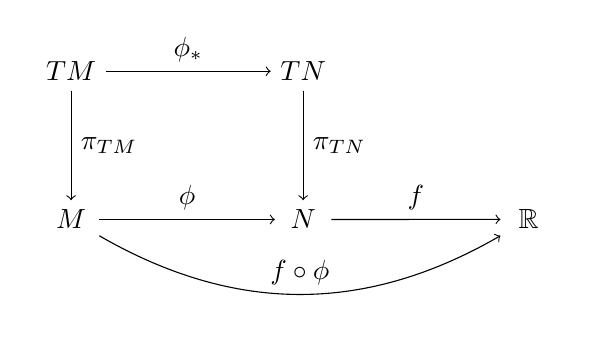
\begin{tikzpicture}
	  \matrix (m) [matrix of math nodes, row sep=4em, column sep=6em, minimum width=2em]
	  {
		TM	&	TN	& \\
		M	&	N	& \mathbb{R} \\
	  };
	  \path[->]  
	  (m-1-1) edge node [auto] {$\phi_\ast$} (m-1-2)
	          edge node [auto] {$\pi_{TM}$} (m-2-1)
	  (m-1-2) edge node [auto] {$\pi_{TN}$} (m-2-2)
	  (m-2-2) edge node [auto] {$f$} (m-2-3)
	  (m-2-1) edge node [auto] {$\phi$} (m-2-2)
	          edge [bend right=30] node [auto] {$f \after \phi$} (m-2-3);
	\end{tikzpicture}
    \caption{\textbf{Push-forward map}: $\phi_\ast$ takes a vector $X \in T_pM$ in the tangent space at the point $p \in M$ to the vector $\phi_\ast(X) \in T_qN$ in the tangent space at the point $\phi(p) = q \in N$, such that the action of $\phi_\ast(X)$ on any smooth function $f \in C^\infty(N)$ results in the same value as the action of $X$ on the function $(f \after \phi)$.}
\end{SCfigure}

\textbf{Note}: If we take an entire fibre at the point $p \in M$, applying $\phi_\ast$ on it remains within the fibre at the point $\phi(p) \in N$. That is \\
\[
\phi_\ast(T_pM) \subseteq T_{\phi(p)}N
\]

\textit{Mnemonic: ``vectors are pushed forward'' across tangent bundles in a manner dictated by the underlying map.}

\textbf{Components of push-forward $\phi_\ast$ w.r.t charts $(U,x) \in \mathcal{A}_M$ and $(V,y) \in \mathcal{A}_N$}: Let $p \in U$ and $\phi(p) \in V$. Since $\cibasis{x^i}_p$ is a vector, we have $\phi_\ast(\cibasis{x^i}_p)$ as a vector in N. Then we can select a component of this vector by using $dy^a$ as follows: \\
\begin{equation} \label{eq_pushForwardComponents}
\underbrace{dy^a\left(\phi_\ast\left(\left(\cibasis{x^i}\right)_p\right)\right)}_{:= \phi^a_{\ast i}} = \phi_\ast\left(\left(\cibasis{x^i}\right)_p\right)y^a = \left(\cibasis{x^i}\right)_p (y^a \after \phi) = \left(\cibasis{x^i}\right)_p (y \after \phi)^a := \left(\cibasis[\hat{\phi}^a]{x^i}\right)_p
\end{equation}

\begin{SCfigure}[5][h]
  \centering
	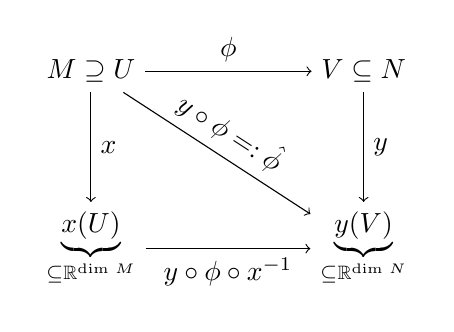
\begin{tikzpicture}
	  \matrix (m) [matrix of math nodes, row sep=4em, column sep=6em, minimum width=2em]
	  {
		M \supseteq U	&	V \subseteq N \\
		\underbrace{x(U)}_{\subseteq \mathbb{R}^{\text{dim }M}}		&	\underbrace{y(V)}_{\subseteq \mathbb{R}^{\text{dim }N}}\\
	  };
	  \path[->]  
	  (m-1-1) edge node [auto] {$\phi$} (m-1-2)
	          edge node [auto] {$x$} (m-2-1)
	          edge node [sloped, anchor=center, above] {$y \after \phi =: \hat{\phi}$} (m-2-2)
	  (m-1-2) edge node [auto] {$y$} (m-2-2)
	  (m-2-1) edge node [below] {$y \after \phi \after x^{-1}$} (m-2-2);
	\end{tikzpicture}
    \caption{Components of push-forward map w.r.t charts $(U,x) \in \mathcal{A}_M$ and $(V,y) \in \mathcal{A}_N$.}
\end{SCfigure}

\begin{theorem}
If $\gamma : \mathbb{R} \to M$ is a curve in $M$, then $\phi \after \gamma : \mathbb{R} \to N$ is a curve in $N$. Then, $\phi_\ast$ pushes the tangent to a curve $\gamma$ (velocity) to the tangent to the curve $(\phi \after \gamma)$, i.e.,
\begin{equation}
\phi_\ast\left(v_{\gamma, p}\right) = v_{(\phi \after \gamma), \phi(p)}
\end{equation}
\end{theorem}
\begin{proof}
Let $p = \gamma(\lambda_0)$. Then $\forall \, f \in C^\infty(N)$,
\begin{align*}
\phi_\ast\left(v_{\gamma, p}\right) f & = v_{\gamma, p} (f \after \phi) && (\text{by Eq.~\ref{eq_defPushForwardMap}}) \\
& = ((f \after \phi) \after \gamma)^\prime (\lambda_0) && (\text{by Eq.~\ref{eq_velocity}}) \\
& = (f \after (\phi \after \gamma))^\prime (\lambda_0) && (\text{by associativity of composition}) \\
& = v_{(\phi \after \gamma), \phi(\gamma(\lambda_0))} f && (\text{by Eq.~\ref{eq_velocity}}) \\
& = v_{(\phi \after \gamma), \phi(p)} f && (\gamma(\lambda_0) = p) \\
\implies \phi_\ast\left(v_{\gamma, p}\right) & = v_{(\phi \after \gamma), \phi(p)}
\end{align*}
\end{proof}

\subsection{Pull-back map}
\begin{definition}
Let $M$ and $N$ be smooth manifolds with cotangent bundles $T^\ast M$ and $T^\ast N$ respectively. Let $\phi : M \to N$ be a smooth map. Then, the \textbf{pull-back map} of $\phi$ is the map
\begin{align}
\phi^{\ast} : & T^\ast N \to T\ast M \nonumber \\
& \omega \mapsto \phi^\ast(\omega) \nonumber \\
\label{eq_defPullBackMap}\text{where } & \phi^\ast(\omega)(X) := \omega (\phi_\ast(X)) && (\forall \, X \in T_pM)
\end{align}
\end{definition}

\textbf{Components of pull-back $\phi^\ast$ w.r.t charts $(U,x) \in \mathcal{A}_M$ and $(V,y) \in \mathcal{A}_N$}: Let $p \in U$ and $\phi(p) \in V$. Since $dy^a$ is a covector, we have $\phi^\ast(dy^a_p)$ as a covector in N. Then we can select a component of this covector by using $\cibasis{x^i}$ as follows: \\
\begin{align*}
\phi^{\ast a} & := \phi^\ast\left(\left(dy^a\right)_{\phi(p)}\right) \left(\left(\cibasis{x^i}\right)_p\right) \\
& = \left(dy^a\right)_{\phi(p)} \phi_\ast \left(\left(\cibasis{x^i}\right)_p\right) && (\text{by Eq.~\ref{eq_defPullBackMap}}) \\
& = \left(\cibasis[\hat{\phi}^a]{x^i}\right)_p  = \phi^a_{\ast i} && (\text{by Eq.~\ref{eq_pushForwardComponents}})
\end{align*}
Thus, the components of the push-forward and pull-back maps are exactly the same.
\begin{align*}
\left(\phi_\ast\left(X\right)\right)^a & = \phi^a_{\ast i} X^i \\
\left(\phi^\ast\left(\omega\right)\right)_i & = \phi^a_{\ast i} \omega_a
\end{align*}
Remember, $a = (1, \dotsc, \text{dim} N)$ and $i = (1, \dotsc, \text{dim} M)$.

Claim: $\phi^\ast(df) = d(f \after \phi)$. 

\textit{Mnemonic: ``covectors are pulled back'' across tangent bundles in a manner dictated by the underlying map.}

\textbf{Important application}:
\begin{definition}
Let $M$ and $N$ be smooth manifolds. Let $\phi : M \injmapto N$ be an injective map. If we know a metric $g$ on $N$, then the \textbf{induced metric} $g_M$ in $M$ is defined using the push-forward map $\phi_\ast$ as follows:
\begin{equation}\label{eq_inducedMetric}
\boxed{g_M(X,Y) := g\left(\phi_\ast(X),\phi_\ast(Y)\right)} \quad \quad (\forall \, X, Y \in T_pM)
\end{equation}
\end{definition}
In terms of components,
\begin{equation}
\left(\left(g_M\right)_{ij}\right)_p = \left(g_{ab}\right)_{\phi(p)} \left(\cibasis[\hat{\phi}^a]{x^i}\right)_{\phi(p)} \left(\cibasis[\hat{\phi}^b]{x^j}\right)_{\phi(p)}
\end{equation}
\textbf{Example}: $N = (\mathbb{R}^3, \stdtop, \mathcal{A})$ and $M = (S^2, \mathcal{O}, \mathcal{A})$, then we can have several injective maps $\phi : S^2 \injmapto \mathbb{R}^3$. For example, $S^2$ could live in $\mathbb{R}^3$ either as a potato or a round sphere. However, suppose $\mathbb{R}^3$ is equipped with the Euclidean metric $g_E$ ...(TODO complete this example)

\subsection{Flow of a complete vector field}
\begin{definition}
Let $X$ be a vector field on a smooth manifold $(M,\mathcal{O},\mathcal{A})$. A curve $\gamma : I \subseteq \mathbb{R} \to M$ is called an \textbf{integral curve of $X$} if 
\[
v_{\gamma,\gamma(\lambda)} = X_{\gamma(\lambda)}
\]
\end{definition}

\begin{definition} A vector field $X$ is \textbf{complete} if all integral curves have $I = \mathbb{R}$ (i.e. domain is all of $\mathbb{R}$).
\end{definition}

\begin{theorem}
Compactly supported smooth vector field is complete.  
\end{theorem}

\begin{definition} The \textbf{flow of a complete vector field $X$} on a manifold $M$ is a 1-parameter family
\begin{align*}
h^X : & \mathbb{R} \times M \to M \\
& (\lambda, p) \mapsto \gamma_p(\lambda)
\end{align*}
where $\gamma_p : \mathbb{R} \to M$ is the integral curve of $X$ with $\gamma(0) = p$. 
\end{definition}

Then for fixed $\lambda \in \mathbb{R}$, $h_{\lambda}^X : M \to M$ is smooth.

\textbf{Picture}: If $S$ is a set of points in $M$, then $h^X_{\lambda}(S)$ can be seen as the new position of these points under the flow $h^X$ after the passage of $\lambda$ units of parameter. In general, $h^X_{\lambda}(S) \neq S (\text{ if } X \neq 0)$.

\subsection{Lie subalgebras of the Lie algebra $(\Gamma(TM), [\cdot, \cdot])$ of vector fields}
We know that $\Gamma(TM) = \lbrace \text{ set of all vector fields } \rbrace$, which can be seen as a $C^{\infty}(M)$-module, or as a $\mathbb{R}$-vector space.

$(\Gamma(TM), [\cdot, \cdot])$ with $[X,Y]$ defined by its action on a function $f$ by $[X,Y] f := X(Yf) - Y(Xf)$ is a Lie algebra since $X,Y \in \Gamma(TM) \implies [X,Y] \in \Gamma(TM)$ and the following properties are satisfied:
\begin{enumerate}[(i)]
\item \textbf{Anticommutativity}: $[X,Y] = -[Y,X]$ 
\item \textbf{Linearity}: $[\lambda X + Z, Y] = \lambda [X,Y] + [Z,Y]$ where $\lambda \in \mathbb{R}$
\item \textbf{Jacobi identity}: $[X,[Y,Z]] + [Z,[X,Y]] + [Y,[Z,X]] = 0$ 
\end{enumerate}

Let $X_1, \dotsc, X_s$ be $s$ (many) vector fields on $M$, such that
\[
\forall i,j \in \lbrace 1,\dotsc,s \rbrace \quad [X_i,X_j] = \underbrace{C^k_{ij} X_k}_{\text{linear combination of }X_k s} \quad \quad \text{where } C^k_{ij} \in \mathbb{R}
\]
$C^k_{ij}$ are called \textbf{structure constants}.

Let $\text{span}_{\mathbb{R}} \lbrace X_1,\dotsc,X_s \rbrace := \lbrace \text{all linear combinations of }X_k \rbrace$. Then $\left(\text{span}_{\mathbb{R}} \lbrace X_1,\dotsc,X_s \rbrace, [\cdot, \cdot]\right)$ is a Lie subalgebra of $(\Gamma(TM), [\cdot, \cdot])$.

\textbf{Example}: In $S^2$, assume that the vector fields $X_1,X_2,X_3$ satisfy $[X_1,X_2] = X_3$, $[X_2,X_3] = X_1$ and $[X_3,X_1] = X_2$. Then $\left(\text{span}_{\mathbb{R}} \lbrace X_1,X_2,X_3 \rbrace, [\cdot, \cdot]\right)$ ($= SO(3)$) is a Lie subalgebra. An instance of vector fields satisfying these conditions is (with $X_i, \theta, \phi$ all taken at a point $p$, and $x^1 = \theta, x^2 = \phi$)
\begin{align*}
& X_1 = - \sin\phi \cibasis{\theta} - \cot\theta \cos\phi \cibasis{\phi} \\
& X_2 = \cos\phi \cibasis{\theta} - \cot\theta \cos\phi \cibasis{\phi} \\
& X_3 = \cibasis{\phi}
\end{align*}
Note that the above is defined on a merely smooth manifold without any additional structure like metric.

\subsection{Symmetry}
\begin{definition}
A finite-dimensional Lie subalgebra $(L,[\cdot,\cdot])$ is said to be a \textbf{symmetry} of a metric tensor field $g$ if
\[
\boxed{g \left( \left(h^X_\lambda\right)_\ast (A), \left(h^X_\lambda\right)_\ast (B) \right) = g(A,B)} \quad\quad (\forall X \text{ (complete vector field) } \in L, \quad \forall \lambda \in \mathbb{R}, \quad \forall A, B \in T_pM)
\]
\end{definition}

In another formulation (using pullback), $\boxed{\left(h^X_\lambda\right)^\ast g = g}$. The pullback of $\phi : M \to M$ on $g$, itself, is defined as follows:
\[
(\phi^\ast g)(A, B) := g(\phi_\ast(A), \phi_\ast(B))
\]

%\textbf{Example}: 

\subsection{Lie derivative}
It can be shown that the following expression is precisely the Lie derivative of $g$ w.r.t a vector field
\begin{equation}
\boxed{\mathcal{L}_X g := \lim_{\lambda \to 0} \frac{\left( h_\lambda^X \right)^\ast g - g}{\lambda}}
\end{equation}
Clearly, $L$ is a symmetry of $g$, iff $\mathcal{L}_X g = 0$.

\begin{definition}
The \textbf{Lie derivative} $\mathcal{L}$ on a smooth manifold $(M, \mathcal{O}, \mathcal{A})$ a pair of a vector field $X$ and a $(p,q)$-tensor field $T$ to a $(p,q)$-tensor field such that
\begin{enumerate}[(i)]
\item $\mathcal{L}_X f = Xf \quad \forall f \in C^{\infty}M$

\item $\mathcal{L}_X Y = [X, Y] \quad\quad \text{ where }X, Y \text{ are vector fields}$
\begin{framed}
This condition sucks in information about the vector field $X$. It is not $C^{\infty}$-linear in the lower index. If it were, the derivative would be independent of values of $X$ at nearby points to the point where derivative is evaluated. This is an important difference between the covariant derivative $\nabla$ and the Lie derivative.
\end{framed}

\item $\mathcal{L}_X (T + S) = \mathcal{L}_X T + \mathcal{L}_X S \quad \text{ where }T, S \text{ are } (p,q) \text{-tensors}$

\item \textbf{Leibnitz rule: } $\mathcal{L}_X T(\omega_1,\dotsc,\omega_p,Y_1,\dotsc,Y_q) = (\mathcal{L}_X T)(\omega_1,\dotsc,\omega_p,Y_1,\dotsc,Y_q) \\
+ T(\mathcal{L}_X \omega_1,\dotsc,\omega_p,Y_1,\dotsc,Y_q) + \dotsb + T(\omega_1,\dotsc,\mathcal{L}_X \omega_p,Y_1,\dotsc,Y_q) \\
+ T(\omega_1,\dotsc,\omega_p,\mathcal{L}_X Y_1,\dotsc,Y_q) + \dotsb + T(\omega_1,\dotsc,\omega_p,Y_1,\dotsc,\mathcal{L}_X Y_q) \quad \text{ where }T \text{ is a }(p,q)\text{-tensor}$
\begin{framed}
Note that for a $(p,q)$-tensor $T$ and a $(r,s)$-tensor $S$, since: \\
$(T \otimes S) (\omega_{(1)}, \dotsc, \omega_{(p+r)}, Y_{(1)}, \dotsc, Y_{(q+s)}) = \\ T(\omega_{(1)}, \dotsc, \omega_{(p)}, Y_{(1)}, \dotsc, Y_{(q)} ) \cdot S( \omega_{(p+1)}, \dotsc, \omega_{(p+r)} , Y_{(q+1)}, \dotsc, Y_{(q+s)})$, \\
Leibnitz rule implies $\mathcal{L}_X (T \otimes S) = (\mathcal{L}_X T) \otimes S + T \otimes (\mathcal{L}_X S)$.
\end{framed}

\item $\mathcal{L}_{X+Y} T = \mathcal{L}_X T + \mathcal{L}_Y T$
\end{enumerate}
\end{definition}

Observe that, in chart $(U,x)$
\[
\left(\mathcal{L}_X Y\right)^i = X^m \cibasis{x^m}(Y^i) - \underbrace{\cibasis{x^s} (X^i)}_{\text{requires knowing } X \text{ around the point} } Y^s
\]
However, for covariant derivative
\[
\left(\nabla_X Y\right)^i = X^m \cibasis{x^m}(Y^i) + \ccf{i}{sm} X^m Y^s
\]
In general, for a $(1,1)$-tensor $T$
\[
\left(\mathcal{L}_X T \right)\indices{^i_j} = X^m \cibasis{x^m}(T\indices{^i_j}) \underbrace{- \cibasis[X^i]{x^s} T\indices{^x_j}}_{('-' \text{ for lower index})} \underbrace{+ \cibasis[X^s]{x^j} T\indices{^i_s}}_{('+' \text{ for upper index})}
\]

\textbf{Application}: As above, it is easy to calculate components of Lie derivative of metric g, $\mathcal{L}_X g$. Thus, by checking whether the derivative equals $0$ or not, it can be determined whether a metric features a symmetry.
 % Symmetry
%\subsection*{Tutorial 11 Symmetry }

\exercisehead{1}\textbf{: True or false?}

\begin{enumerate}
\item[(a)]
\begin{itemize}
\item
\item $\phi^*:T^*N \to T*M$ i.e. $\phi^*\nu(X) = \nu(\phi_*X)$ for smooth $\phi:M \to N$, so the pullback of a covector $\nu \in T^*N$ maps to a covector in $T*M$.  
\item
\item
\item
\item
\end{itemize}
\item[(b)]
\item[(c)]
\end{enumerate}

\exercisehead{2}: Pull-back and push-forward

\questionhead{}Let's check this locally
\[
\begin{aligned}
  & \phi^*(df)(X) = (df)(\phi_*X) = (df)(X^i \frac{ \partial y^j}{\partial x^i} \frac{ \partial }{ \partial y^j}  ) = X^i \frac{ \partial y^j}{ \partial x^i} \frac{ \partial f}{ \partial y^j} \text{ where } 
  & \phi_* X = X^i \frac{ \partial y^j}{ \partial x^i} \frac{ \partial }{ \partial y^j} \\ 
  & d(\phi^*f)(X) = d(f(\phi))(X) = \frac{ \partial f}{ \partial y^j} \frac{ \partial y^j}{ \partial x^i } dx^i(X) = X^i \frac{ \partial y^j}{ \partial x^i} \frac{ \partial f}{ \partial y^j}
\end{aligned}
\]
So 
\[
\boxed{ \phi^*(df) = d(\phi^* f)  } \quad \quad \, \forall \, p \in M , \, \, \forall \, X \in \mathfrak{X}(M)
\]
The big idea is that this is a showing of the \textbf{naturality} of the pullback $\phi^*$ with $d$, i.e. that this commutes:

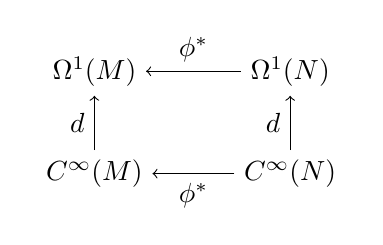
\begin{tikzpicture}
  \matrix (m) [matrix of math nodes, row sep=2em, column sep=3em, minimum width=1em]
  {
 \Omega^1(M)  &  \Omega^1(N)   \\
C^{\infty}(M) & C^{\infty}(N)  \\  };
%  \path[-stealth]
  \path[->]
  (m-1-2) edge node [above] {$\phi^*$} (m-1-1)
%  edge node [left] {$\text{ev}_0$} (m-2-2)
%  (m-1-1) edge node [left] {$\alpha$} (m-2-1)
  (m-2-2) edge node [auto] {$d$} (m-1-2)
%  edge node [below] {$\pi_M$} (m-2-2);
  edge node [auto] {$\phi^*$} (m-2-1)
  (m-2-1) edge node [left] {$d$} (m-1-1);
\end{tikzpicture}

\questionhead{}

\[
(\phi_*)^a_{ \, \, b} := (dy^a)(\phi_*( \frac{ \partial }{ \partial x^b } ) )
\]
\[
\text{ Let } g \in C^{\infty}(N)
\]
\[
\begin{gathered}
  \phi_* \left( \frac{ \partial }{ \partial x^b} \right) g = \frac{ \partial x^b} g\phi(p) = \frac{ \partial }{ \partial x^b} g\phi x^{-1}x(p) = \frac{ \partial }{ \partial x^b}(gyy^{-1}\phi x^{-1})(x) = \\
  = \frac{ \partial }{ \partial x^b}(gy^{-1}(y\phi x^{-1}(x(p))) ) = \left. \frac{ \partial g}{ \partial y}^b \right|_y \left. \frac{ \partial y^a}{ \partial x^b} \right|_x = \frac{ \partial y^a}{ \partial x^b} \frac{ \partial g}{ \partial y^a}
\end{gathered}
\]
Then 
\[
\phi_*\left( \frac{ \partial }{ \partial x^b} \right) = \frac{ \partial y^a}{ \partial x^b} \frac{ \partial }{ \partial y^a}
\]
and so 
\[
(\phi_*)^a_{ \, \, b} = \frac{ \partial y^a}{ \partial x^b}
\]

\questionhead{}

\exercisehead{3}\textbf{:Lie derivative-the pedestrian way}

\questionhead{} While it is true that $\forall \, p \in S^2$, for $x(p) = (\theta, \varphi)$, and $(yix^{-1})(\theta,\varphi) = (y^1,y^2,y^3) \in \mathbb{R}^3$ and that, at this point $p$, $(y^1)^2/a^2 + (y^2)^2/b^2 +(y^3)^2/c^3 = 1$, this doesn't imply (EY: 20150321 I think) that, globally, it's an ellipsoid (yet).  In the familiar charts given, \\
spherical chart $(U,x) \in \mathcal{A}$ and \\
$(\mathbb{R}^3, y=\text{id}_{\mathbb{R}^3}) \in \mathcal{B}$ \\
it looks like an ellipsoid, but change to another choice of charts, and it could look something very different.  

\questionhead{}

Equip $(\mathbb{R}^3, \mathcal{O}_{\text{st}}, \mathcal{B})$ with the Euclidean metric $g$, and pullback $g$.  

Note that the pullback of the inclusion from $\mathbb{R}^3$ onto $S^2$ for the Euclidean metric is the following:
\[
i^* g\left( \frac{ \partial }{ \partial \theta^i }, \frac{ \partial }{ \partial \theta^j} \right) = g\left( i_*\frac{ \partial }{ \partial \theta^i }, i_*\frac{ \partial }{ \partial \theta^j} \right) = g\left( \frac{ \partial x^a}{ \partial \theta^i} \frac{ \partial }{ \partial x^a} , \frac{ \partial x^b}{ \partial \theta^j} \frac{ \partial }{ \partial x^b } \right) = g_{ab} \frac{ \partial x^a}{ \partial \theta^i} \frac{ \partial x^b}{ \partial \theta^j} 
\]
With $g_{ab}=\delta_{ab}$, the usual Euclidean metric, this becomes the following:
\[
g^{\text{ellipsoid}}_{ij} = \frac{ \partial x^a}{ \partial \theta^i} \frac{ \partial x^a}{ \partial \theta^j} 
\]

At this point, one should get smart (we are in the 21st century) and use some sort of CAS (Computer Algebra System). I like Sage Math (version 6.4 as of 20150322).  I also like the Sage Manifolds package for Sage Math.  

I like Sage Math for the following reasons:
\begin{itemize}
\item Open source, so it’s open and freely available to anyone, which fits into my principle of making online education open and freely available to anyone, anytime
\item Sage Math structures everything in terms of Category Theory and Categories and Morphisms naturally correspond to Classes and Class methods or functions in Object-Oriented Programming in Python and they’ve written it that way
\end{itemize}
and I like Sage Manifolds for roughly the same reasons, as manifolds are fit into a category theory framework that’s written into the Python code.  e.g.

{\small \begin{verbatim}
sage: S2 = Manifold(2, 'S^2', r'\mathbb{S}^2', start_index=1) ; print S2
sage: print S2
2-dimensional manifold 'S^2'
sage: type(S2)
<class 'sage.geometry.manifolds.manifold.Manifold_with_category'>
\end{verbatim}}

With code (I’ve provided for convenience; you can make your own as I wrote it based upon to example of $S^2$ on the sagemanifolds documentation website page), load it and do the following:

cf. \url{https://github.com/ernestyalumni/diffgeo-by-sagemnfd/blob/master/S2.sage} \\
\url{http://sagemanifolds.obspm.fr/examples.html}

{\scriptsize \begin{verbatim}
sage: load("S2.sage")
sage: U_ep = S2.open_subset('U_{ep}')
sage: eps.<the,phi> = U_ep.chart()
sage: a = var(“a”)
sage: b = var(“b”)
sage: c = var("c")
sage: inclus = S2.diff_mapping(R3, {(eps, cart): [ a*cos(phi)*sin(the), b*sin(phi)*sin(the),c*cos(the) ]} , name="inc",latex_name=r'\mathcal{i}')
sage: inclus.pullback(h).display()
inc_*(h) = (c^2*sin(the)^2 + (a^2*cos(phi)^2 + b^2*sin(phi)^2)*cos(the)^2) dthe*dthe - (a^2 - b^2)*cos(phi)*cos(the)*sin(phi)*sin(the) dthe*dphi 
- (a^2 - b^2)*cos(phi)*cos(the)*sin(phi)*sin(the) dphi*dthe + (b^2*cos(phi)^2 + a^2*sin(phi)^2)*sin(the)^2 dphi*dphi
sage: inclus.pullback(h)[2,2].expr()
(b^2*cos(phi)^2 + a^2*sin(phi)^2)*sin(the)^2
\end{verbatim}
}
A new open subset $U_{\text{ep}}$ was declared in $S^2$, a new chart $(U_{\text{ep}}, (\theta,\phi))$ was declared, the constants, $a,b,c$, were declared, and the inclusion map given in the problem
\[
y\circ \mathfrak{i} \circ x^{-1} : (\theta, \phi) \mapsto ( a\cos{\phi} \sin{\theta}, b \sin{\phi} \sin{\theta}, c\cos{\theta})
\]
Then the pullback of the inclusion map $\mathcal{i}$ was done on the Euclidean metric $h$, defined earlier in the file \begin{verbatim}S2.sage\end{verbatim}.  Then one can access the components of this metric and do, for example, \begin{verbatim}simplify_full(),full_simplify(), reduce_trig()\end{verbatim} on the expression.  

In Python, I could easily do this, and give an answer quick in LaTeX:

%{\scriptsize 
\begin{verbatim}
sage: for i in range(1,3): 
....:     for j in range(1,3):
....:         print inclus.pullback(h)[i,j].expr()
....:         latex(inclus.pullback(h)[i,j].expr() )
....:         
c^2*sin(the)^2 + (a^2*cos(phi)^2 + b^2*sin(phi)^2)*cos(the)^2
\end{verbatim}
(EY: I'll suppress the LaTeX output but this sage math function gives you LaTeX code)
%c^{2} \sin\left(\mathit{the}\right)^{2} + {\left(a^{2} \cos\left(\phi\right)^{2} + 
%b^{2} \sin\left(\phi\right)^{2}\right)} \cos\left(\mathit{the}\right)^{2}
%-(a^2 - b^2)*cos(phi)*cos(the)*sin(phi)*sin(the)
%-{\left(a^{2} - b^{2}\right)} \cos\left(\phi\right) \cos\left(\mathit{the}\right) \sin\left(\phi\right) \sin\left(\mathit{the}\right)
%-(a^2 - b^2)*cos(phi)*cos(the)*sin(phi)*sin(the)
%-{\left(a^{2} - b^{2}\right)} \cos\left(\phi\right) \cos\left(\mathit{the}\right) \sin\left(\phi\right) \sin\left(\mathit{the}\right)
%(b^2*cos(phi)^2 + a^2*sin(phi)^2)*sin(the)^2
%{\left(b^{2} \cos\left(\phi\right)^{2} + a^{2} \sin\left(\phi\right)^{2}\right)} \sin\left(\mathit{the}\right)^{2}
%
%

and so

\[
\boxed{ \begin{gathered}
 i^* g = c^{2} \sin\left(\mathit{the}\right)^{2} + {\left(a^{2} \cos\left(\phi\right)^{2} + b^{2} \sin\left(\phi\right)^{2}\right)} \cos\left(\mathit{the}\right)^{2} d\theta \otimes d\theta + \\
-2 {\left(a^{2} - b^{2}\right)} \cos\left(\phi\right) \cos\left(\mathit{the}\right) \sin\left(\phi\right) \sin\left(\mathit{the}\right) d\theta \otimes d\phi +  \\
 + {\left(b^{2} \cos\left(\phi\right)^{2} + a^{2} \sin\left(\phi\right)^{2}\right)} \sin\left(\mathit{the}\right)^{2} d\phi \otimes d\phi 
\end{gathered} }
\]

\questionhead{}

{\small
\begin{verbatim}
sage: polar_vees = eps.frame()
sage: X_1 = - sin(phi) * polar_vees[1] - cot( the ) * cos(phi) * polar_vees[2]
sage: X_2 = cos( phi ) * polar_vees[1] - cot( the ) * sin( phi) * polar_vees[2]
sage: X_3 = polar_vees[2]
sage: X_2.lie_der(X_1).display()
(cos(the)^2 - 1)/sin(the)^2 d/dphi
sage: X_3.lie_der(X_1).display()
cos(phi) d/dthe - cos(the)*sin(phi)/sin(the) d/dphi
sage: X_3.lie_der(X_2).display()
sin(phi) d/dthe + cos(phi)*cos(the)/sin(the) d/dphi
\end{verbatim}
}

Indeed, one can check on a scalar field $f_{\text{eps}} \in C^{\infty}(S^2)$:
{\small
\begin{verbatim}
sage: f_eps = S2.scalar_field({eps: function('f', the, phi ) }, name='f' )
sage: (X_1( X_2(f_eps)) - X_2(X_1(f_eps) ) ).display()
U_{ep} --> R
(the, phi) |--> -D[1](f)(the, phi)
sage: X_2.lie_der(X_1) == -X_3
True
sage: X_3.lie_der(X_1) == X_2
True
sage: X_3.lie_der(X_2) == -X_1
True
\end{verbatim}
}

\[
\Longrightarrow \boxed{ [X_i, X_j] = -\epsilon_{ijk}X_k }
\]
So $\text{span}_{\mathbb{R}} \lbrace X_1,X_2,X_3 \rbrace$ equipped with $[ \, , \, ]$ constitute a Lie subalgebra on $S^2$ (It's closed under $[ \, , \, ]$



\section{Integration}
\begin{framed}
This lecture will be the completion of our ``lift'' of analysis on charts to the manifold level. We want to be able to integrate a function $f$ over a manifold $M$. This $\int_{M} f$ will be an important tool for writing down the action on Einstein Equations.

However, to define integral we need a mild new structure on the smooth manifold $\mfd$. It requires \\
(i) a choice of a certain tensor field, the so-called \textbf{volume form} and \\
(ii) a restriction on the atlas $\A$, which is called '\textbf{orientation}'.
\end{framed}

\subsection{Review of integration on $\mathbb{R}^d$}
We review this because this is what, after all, happens on charts; and we want to use this knowledge to have a well-defined integration on manifolds.
\begin{enumerate}[a)]
\item If $F : \R \to \R$, we assume a notion of integration is known. We define an integral over an interval $(a,b)$ as follows: \\
\[
\int_{(a,b)} F := \int_a^b dx \, F(x) \quad\quad \text{(which is understood in terms of, say, Riemann's integral)}.
\]

\item If $F : \R^k \to \R$, then
\begin{enumerate}[(i)]
\item on a box-shaped domain, $Box = (a,b) \times (c,d) \times \dotsb \times (u,v) \subseteq \R^k$, the integral on the box is a series of integrals which have to be evaluated one after the other as follows \\
\[
\int_{Box} F := \int_a^b dx^1 \int_c^d dx^2 \dotsi \int_u^v dx^k \, F(x^1, x^2, \dotsc, x^k)
\]
\item for other domains, $G \subseteq \R^k$, we first introduce an \textbf{indicator function} $\mu_G : \R^k \to \R$ such that
\[
\mu_G(x) = \begin{cases}
               1, \quad \quad x \in G \\
               0, \quad \quad x \not\in G
            \end{cases}
\]
and then define
\[
\int_{G} F := \int_{-\infty}^{+\infty} dx^1 \int_{-\infty}^{+\infty} dx^2 \dotsi \int_{-\infty}^{+\infty} dx^k \, \mu_G(x) \cdot F(x^1, x^2, \dotsc, x^k)
\]
While this may not be a practical definition, it tells us what we mean by an integral over a function from $\R^k$ to $\R$ over an arbitrary domain $G$.
\end{enumerate}
\end{enumerate}

\textit{\textbf{Note}: All of the above comes with the disclaimer '\textbf{if the integral exists}' since there could be many issues that do not allow the existence of the integral as defined above.}

\textbf{Change of variables}, which may also be called integration by substitution.

\begin{theorem}
If $F : \R^k \ni G \to \R$ and $\phi : preim_\phi(G) (\in \R^k) \to G$, then
\[
\int_G F(x) = \int_{preim_\phi(G)} \underbrace{\left\lvert det(\partial x)(y) \right\rvert}_{\text{Jacobian of }\phi} \cdot (F \after \phi)(y)
\]
\end{theorem}

\begin{tikzpicture}
  \matrix (m) [matrix of math nodes, row sep=4em, column sep=6em, minimum width=2em]
  {
    \R^k \ni preim_\phi(G) & G \in \R^k \\
    & \R \\
  };
  \path[->]
  (m-1-1) edge node[auto] {$\phi$} (m-1-2)
          edge node[sloped, anchor=center, below] {$F \after \phi$} (m-2-2)
  (m-1-2) edge node[auto] {$F$} (m-2-2);
\end{tikzpicture}

\textbf{Example}: Consider the domain $G \subset \R^2$, which includes the entire $R^2$ except the x-axis. Let
\begin{align*}
\phi : & \R^+ \times \lbrace(0,\pi) \cup (\pi,2\pi)\rbrace \to G \\
& (r, \varphi) \mapsto (r\cos\varphi, r\sin\varphi)
\end{align*}
Thus, $G$ is in Cartesian coordinates and $preim_\phi(G)$ is in polar coordinates. Let us calculate the Jacobian.
\begin{align*}
(\partial_a x^b) (r, \varphi) & = \begin{vmatrix}
\cos\varphi & \sin\varphi \\
-r\sin\varphi & r\cos\varphi
\end{vmatrix} \\
det(\partial_a x^b) (r, \varphi) & = r \\
\implies \int_G \underbrace{dx^1 \, dx^2}_{\text{volume element}} \, F(x^1,x^2) & = \int_0^\infty \int_0^{2\pi} \underbrace{dr \, d\varphi \, r}_{\text{volume element}} F(r\cos\varphi, r\sin\varphi)
\end{align*}

\subsection{Integration on one chart}
Let $\mfd$ be a smooth manifold, $f : M \to \R$ and choose charts $(U,x), (U,y) \in \A$

\begin{tikzpicture}
  \matrix (m) [matrix of math nodes, row sep=5em, column sep=7em, minimum width=2em]
  {
    y(U) \in \R^k &  \\
    U & \R \\
    x(U) \in \R^k &  \\
  };
  \path[->]
  (m-2-1) edge node[auto] {$f$} (m-2-2)
          edge node[auto] {$y$} (m-1-1)
          edge node[auto] {$x$} (m-3-1)
  (m-1-1) edge node[sloped, anchor=center, above] {$f_{(y)} := f \after y^{-1}$} (m-2-2)
  (m-3-1) edge node[sloped, anchor=center, below] {$f_{(x)} := f \after x^{-1}$} (m-2-2)
  (m-3-1) edge [bend left=40] node[left] {$y \after x^{-1}$} (m-1-1);
\end{tikzpicture}

Consider $\int_U f$
\[
\int_U f := \int_{x(U)} d^k\alpha \, f_{(x)}(\alpha)
\]
\subsection{Volume forms}

\begin{definition}
On a smooth manifold $(M,\mathcal{O},\mathcal{A})$ \\
a $(0,\text{dim}M)$-tensor field $\Omega$ is called a \underline{volume form} if 
\begin{enumerate}
\item[(a)] $\Omega$ vanishes nowhere (i.e. $\Omega \neq 0 \, \, \forall \, p \in M$) 
\item[(b)] totally antisymmetric 
\[
\Omega(\dots , \underbrace{X}_{i\text{th}} , \dots , \underbrace{Y}_{j\text{th}} \dots ) = - \Omega(\dots , \underbrace{Y}_{i\text{th}} , \dots , \underbrace{X}_{j\text{th}} \dots )
\]
\end{enumerate}

In a chart: 
\[
\Omega_{i_1 \dots i_d} = \Omega_{ [i_1 \dots i_d ]}
\]
\end{definition}

\underline{Example} $(M,\mathcal{O}, \mathcal{A},g)$ metric manifold

construct volume form $\Omega$ from $g$

In \underline{any} chart: $(U,x)$

\[
\Omega_{i_1 \dots i_d} := \sqrt{ \text{det}(g_{ij}(x)) } \epsilon_{i_1 \dots i_d} 
\]
where \textbf{Levi-Civita symbol} $\epsilon_{i_1 \dots i_d}$ is \underline{defined} as $\begin{aligned} & \quad \\ 
& \epsilon_{123 \dots d} = +1 \\ 
& \epsilon_{1\dots d} = \epsilon_{[i_1 \dots i_d]} \end{aligned}$

\begin{proof} (well-defined) Check: What happens under a change of charts
\[
\begin{aligned}
\Omega(y)_{i_1 \dots i_d} & = \sqrt{ \text{det}(g(y)_{ij}) } \epsilon_{i_1 \dots i_d} = \\
& = \sqrt{ \text{det}(g_{mn}(x) \frac{ \partial x^m}{ \partial y^i} \frac{ \partial x^n}{ \partial y^j} )} \frac{ \partial y^{m_1} }{ \partial x^{i_1} } \dots \frac{ \partial y^{m_d}}{ \partial x^{i_d}} \epsilon_{ [m_1 \dots m_d] } = \\
& = \sqrt{ | \text{det}g_{ij}(x) | } \left| \text{det}\left( \frac{ \partial x}{ \partial y} \right) \right| \text{det}\left( \frac{ \partial y}{ \partial x} \right) \epsilon_{i_1 \dots i_d} = \sqrt{ \text{det}g_{ij}(x)} \epsilon_{i_1 \dots i_d} \text{sgn}\left( \text{det}\left( \frac{ \partial x}{ \partial y} \right) \right)
\end{aligned}
\]
\end{proof}

EY : 20150323 

Consider the following:
\[
\begin{aligned}
\Omega(y)(Y_{(1)} \dots Y_{(d)} ) & = \Omega(y)_{i_1 \dots i_d}Y_{(1)}^{i_1} \dots Y_{(d)}^{i_d} =  \\
& = \sqrt{ \text{det}(g_{ij}(y)) } \epsilon_{i_1 \dots i_d} Y^{i_1}_{(1)} \dots Y^{i_d}_{(d)} = \\
& = \sqrt{ \text{det}(g_{mn}(x)) \frac{ \partial x^m}{ \partial y^i} \frac{ \partial x^n }{ \partial y^j} } \epsilon_{i_1 \dots i_d} \frac{ \partial y^{i_1}}{ \partial x^{m_1} } \dots \frac{ \partial y^{i_d} }{ \partial x^{m_d} } X^{m_1} \dots X^{m_d}  = \\
& = \sqrt{ \text{det}(g_{mn}(x))\frac{ \partial x^m}{ \partial y^i} \frac{ \partial x^n}{ \partial y^j}} \text{det}\left( \frac{ \partial y}{ \partial x}\right) \epsilon_{m_1 \dots m_d} X^{m_1} \dots X^{m_d} = \\
& = \sqrt{ \text{det}(g_{mn}(x)) } \left| \text{det}\left( \frac{ \partial x}{ \partial y} \right) \right| \text{det}\left( \frac{ \partial y}{ \partial x} \right) \epsilon_{m_1 \dots m_d} X^{m_1} \dots X^{m_d} = \\
& = \sqrt{\text{det}(g_{mn}(x))} \epsilon_{m_1 \dots m_d} \text{sgn}\left(\text{det}\left( \frac{ \partial x}{ \partial y} \right) \right) X^{m_1} \dots X^{m_d} = \text{sgn}(\text{det}\left( \frac{ \partial x}{ \partial y} \right)) \Omega_{m_1 \dots m_d}(x) X^{m_1} \dots X^{m_d}
\end{aligned}
\]

If $\text{det}\left( \frac{ \partial y}{ \partial x} \right) > 0$, 
\[
\Omega(y)(Y_{(1)} \dots Y_{(d)})  = \Omega(x)(X_{(1)} \dots X_{(d)} )
\]
This works also if Levi-Civita symbol $\epsilon_{i_1\dots i_d}$ doesn't change at all under a change of charts. (around 42:43 \url{https://youtu.be/2XpnbvPy-Zg})

\hrulefill

Alright, let's require, \\
\phantom{\quad \, } restrict the smooth atlas $\mathcal{A}$ \\
\phantom{\quad \quad \, } to a subatlas ($\mathcal{A}^{\uparrow}$ still an atlas) 
\[
\mathcal{A}^{\uparrow} \subseteq \mathcal{A}
\]
s.t. $\forall \, (U,x), (V,y)$ have chart transition maps $\begin{aligned} & \quad \\ 
& y\circ x^{-1} \\ 
& x\circ y^{-1} \end{aligned}$

s.t. $\text{det}\left( \frac{ \partial y}{ \partial x} \right) >0$  \\
\phantom{ \quad \, } such $\mathcal{A}^{\uparrow} $ called an \textbf{oriented} atlas 

\[
(M, \mathcal{O}, \mathcal{A},g) \Longrightarrow (M,\mathcal{O},\mathcal{A}^{\uparrow} ,g)
\]
Note: associated bundles.

Note also:
$ \text{det}\left( \frac{ \partial y^b}{ \partial x^a} \right) = \text{det}(\partial_a(y^bx^{-1}))$ \phantom{ \quad \quad \, } $\frac{ \partial y^b}{ \partial x^a}$ is an endomorphism on vector space $V$.  $\begin{aligned} & \quad \\ 
& \varphi : V \to V \\
& \text{det}\varphi \quad \, \text{ independent of choice of basis } \end{aligned}$

\phantom{\quad \quad \, } $g$ is a $(0,2)$ tensor field, not endomorphism (not independent of choice of basis) $\sqrt{ |\text{det}(g_{ij}(y)) | }$

\begin{definition} $\Omega$ be a volume form on $(M,\mathcal{O}, \mathcal{A}^{\uparrow} )$ and consider chart $(U,x)$ 
\begin{definition} $\omega_{(X)} := \Omega_{i_1\dots i_d} \epsilon^{i_1\dots i_d}$
same way $\begin{aligned} & \quad \\ 
& \epsilon^{12 \dots d} = +1 \\ 
& \epsilon^{[\dots ]} \end{aligned}$

one can show

\[
\boxed{ \omega_{(y)} = \text{det}\left( \frac{ \partial x}{ \partial y} \right) \omega_{(x)} } \quad \quad \, \text{ scalar density }
\]
\end{definition}
\end{definition}

\subsection{Integration on \underline{one} chart domain $U$}

\begin{definition}
\begin{equation}
\boxed{ \int_U f :\overset{ (U,y) }{=} \int_{y(U)} d^d\beta \omega_{(y)}(y^{-1}(\beta)) f_{(y)}(\beta) }
\end{equation}
\end{definition}

\begin{proof}: Check that it's (well-defined), how it changes under change of charts
\[
\begin{gathered}
\int_U f :\overset{ (U,y) }{=} \int_{y(U)} d^d\beta \omega_{(y)}(y^{-1}(\beta)) f_{(y)}(\beta) = \underset{ (U,y)}{=} \int_{x(U)} \int d^d\alpha \left| \text{det}\left( \frac{ \partial y }{ \partial x}\right) \right| f_{(x)}(\alpha) \omega_{(x)}(x^{-1}(\alpha) \text{det}\left( \frac{ \partial x}{ \partial y } \right) = \\
= \int_{x(U)} d^d \alpha \omega_{(x)}(x^{-1}(x)) f_{(x)}(\alpha)
\end{gathered}
\]
\end{proof}

On an oriented metric manifold $(M,\mathcal{O}, \mathcal{A}^{\uparrow}, g)$
\[
\int_Uf:= \int_{x(U)} d^d\alpha  \underbrace{  \sqrt{ \text{det}(g_{ij}(x))(x^{-1}(\alpha)) } }_{\sqrt{g}}  f_{(x)}(\alpha)
\]

\subsection{Integration on the entire manifold}

 % Integration
\section{Lecture 13: Relativistic spacetime}

Recall, from Lecture 9, the definition of Newtonian spacetime
\[
(M, \mathcal{O}, \mathcal{A}, \nabla, t) \quad \quad \quad \, \begin{aligned}
& \nabla \text{ torsion free } \\
& t \in C^{\infty}(M) \\ 
& dt \neq 0 \\
& \nabla dt = 0   \quad \, \text{ (uniform time) }
\end{aligned}
\]
and the definition of relativistic spacetime (before Lecture )


\[
(M, \mathcal{O}, \mathcal{A}^{\uparrow}, \nabla, g, T ) \quad \quad \quad \, \begin{aligned}
& \nabla \text{ torsion-free } \\
& g \text{ Lorentzian metric} (+---) \\ 
& T \text{ time-orientation }
\end{aligned}
\]

\subsection{Time orientation}

\begin{definition}
  $(M,\mathcal{O},\mathcal{A}^{\uparrow},g)$ a Lorentzian manifold.  Then a time-orientation is given by a vector field $T$ that 
\begin{enumerate}
\item[(i)] does \textbf{not} vanish anywhere 
\item[(ii)] $g(T,T)>0$
\end{enumerate}
\end{definition}

Newtonian vs. relativistic \\
Newtonian \\
$X$ was called future-directed if 
\[
dt(X) >0
\]
$\forall \, p \in M$, take half plane, half space of $T_pM$ \\
also stratified atlas so make planes of constant $t$ straight \\
relativistic \\
half cone $\forall \, p, q \in M$, half-cone $\subseteq T_pM$ \\

This definition of \underline{spacetime}

Question \\
I see how the cone structure arises from the new metric. I don't understand however, how the $T$, the time orientation, comes in \\

Answer \\
$(M,\mathcal{O}, \mathcal{A},g)$ $g \xleftarrow (+---)$

requiring $g(X,X)>0$, select cones \\
$T$ chooses which cone \\

This definition of \underline{spacetime} has been made to enable the following physical postulates:
\begin{enumerate}
\item[(P1)] The worldline $\gamma$ of a \underline{massive} particle satisfies
\begin{enumerate}
  \item[(i)] $g_{\gamma(\lambda)}(v_{\gamma, \gamma(lambda)} , v_{\gamma,\gamma(\lambda)} ) >0$
  \item[(ii)] $g_{\gamma(\lambda)}(T, v_{\gamma,\gamma(\lambda)}) >0$
\end{enumerate}
\item[(P2)] Worldlines of \underline{massless} particles satisfy
\begin{enumerate}
\item[(i)] $g_{\gamma(\lambda)}(v_{\gamma,\gamma(\lambda)}, v_{\gamma,\gamma(\lambda)}) = 0$
\item[(ii)] $g_{\gamma(\lambda)}(T,v_{\gamma,\gamma(\lambda)}) >0$
\end{enumerate}
\underline{picture}: spacetime:
\end{enumerate}

Answer (to a question) $T$ is a smooth vector field, $T$ determines future vs. past, ``general relativity: we have such a time orientation; smoothness makes it less arbitrary than it seems'' -FSchuller,


\underline{Claim}: $9/10$ of a metric are determined by the cone

spacetime determined by distribution, only one-tenth error 

\subsection{Observers} $(M,\mathcal{O}, \mathcal{A}^{\uparrow},\nabla ,g, T)$
\begin{definition}
  An \underline{observer} is a worldline $\gamma$ with
\[
\begin{aligned}
  & g(v_{\gamma}, v_{\gamma}) >  0 \\ 
  & g(T,v_{\gamma}) > 0 
\end{aligned}
\]
together with a choice of basis
\[
v_{\gamma,\gamma(\lambda)} \equiv e_0(\lambda) , e_1(\lambda), e_2(\lambda), e_3(\lambda)
\]
of each $T_{\gamma(\lambda)}M$ where the observer worldline passes, if $g(e_a(\lambda), e_b(\lambda)) = \eta_{ab} = \left[ \begin{matrix} 1 & & & \\ & -1 & & \\ & & -1 & \\ & & & -1 \end{matrix} \right]_{ab}$

\underline{precise}: observer $=$ \underline{smooth} curve in the frame bundle $LM$ over $M$
\end{definition}

\subsubsection{Two physical postulates}

\begin{enumerate}
  \item[(P3)] A \textbf{clock} carried by a specific observer $(\gamma, e)$ will measure a \textbf{time}
\[
\tau := \int_{\lambda_0}^{\lambda_1} d\lambda \sqrt{ g_{\gamma(\lambda)}(v_{\gamma,\gamma(\lambda)}, v_{\gamma,\gamma(\lambda)}) }
\]
between the two ``\underline{events}''
\[
\gamma(\lambda_0) \quad \quad \quad \, \text{ ``start the clock'' }
\]
and 
\[
\gamma(\lambda_1) \quad \quad \quad \, \text{ ``stop the clock'' }
\]
\underline{Compare} with Newtonian spacetime:
\[
t(p)=7
\]

Thought bubble: \underline{proper time/eigentime} $\tau$

\underline{Application/Example.}
$\begin{aligned}
& M = \mathbb{R}^4 \\ 
 & \mathcal{O} = \mathcal{O}_{\text{st}} \\
  & \mathcal{A} \ni (\mathbb{R}^4, \text{id}_{\mathbb{R}^4} ) \\ 
  & g : g_{(x)ij} = \eta_{ij} \quad \, ; \quad \quad \, T_{(x)}^i =(1,0,0,0)^i
\end{aligned}
$
\[
\Longrightarrow \Gamma_{(x) \, \, jk }^i = 0 \text{ everywhere }
\]
$\Longrightarrow (M,\mathcal{O}, \mathcal{A}^{\uparrow},g,T,\nabla)$ \quad \, $\text{Riemm}=0$ \\
$\Longrightarrow $ spacetime is flat

This situation is called special relativity.

Consider two observers: 
\[
\begin{aligned} & 
\begin{aligned}
& \gamma : (0,1) \to M \\ 
 & \gamma_{(x)}^i = (\lambda , 0 ,0  ,0 )^i \end{aligned} \\
& 
\begin{aligned}
  & \delta :(0,1) \to M \\
\alpha \in (0,1) :   & \delta_{(x)}^i = \begin{cases} ( \lambda , \alpha \lambda , 0 , 0)^i & \lambda \leq \frac{1}{2} \\ 
    (\lambda, (1-\lambda)\alpha, 0,0)^i & \lambda > \frac{1}{2} \end{cases}
\end{aligned}
\end{aligned}
\]
let's calculate:
\[
\begin{aligned}
  & \tau_{\gamma}:= \int_0^1 \sqrt{ g_{(x)ij} \dot{\gamma}^i_{(x)} \dot{\gamma}^j_{(x)} } = \int_0^1 d\lambda 1 = 1 \\
  & \tau_{\delta} := \int_0^{1/2} d\lambda \sqrt{ 1- \alpha^2} + \int_{1/2}^1 \sqrt{ 1^2 - (-\alpha)^2 } = \int_0^1 \sqrt{ 1 - \alpha^2 } = \sqrt{ 1 - \alpha^2}
\end{aligned}
\]
Note: piecewise integration

Taking the clock postulate (P3) seriously, one better come up with a realistic clock design that supports the postulate. 
\underline{idea}.

2 little mirrors
\item[(P4)] \underline{Postulate}

Let $(\gamma, e)$ be an observer, and \\
$\delta$ be a \emph{massive} particle worldline that is parametrized s.t. $g(v_{\gamma}, v_{\gamma})=1$ (for parametrization/normalization convenience)

Suppose the observer and the particle \emph{meet} somewhere (in spacetime)
\[
\delta(\tau_2) = p = \gamma(\tau_1)
\]

\emph{This} observer measures the 3-velocity (spatial velocity) of this particle as 
\begin{equation}\label{Eq:spatialv}
v_{\delta}: \epsilon^{\alpha}( v_{\delta, \delta(\tau_2)} ) e_{\alpha} \quad \quad \quad \, \alpha =1,2,3
\end{equation}
where $\epsilon^0, \boxed{ \epsilon^1,\epsilon^2,\epsilon^3}$ is the unique dual basis of $e_0,\boxed{ e_1,e_2,e_3}$
\end{enumerate}

EY:20150407

There might be a major correction to Eq. (\ref{Eq:spatialv}) from the Tutorial 14 : Relativistic spacetime, matter, and Gravitation, see the second exercise, Exercise 2, third question:
\begin{equation}
v := \frac{ \epsilon^{\alpha}({v}_{\delta} ) }{ \epsilon^0({v}_{\delta}) } e_{\alpha}
\end{equation}

\underline{Consequence}:
An observer $(\gamma, e)$ will extract quantities measurable in his laboratory from objective spacetime quantities always like that.

\underline{Ex}: $F$ Faraday $(0,2)$-tensor of electromagnetism:

\[
F(e_a,e_b) = F_{ab} = \left[ \begin{matrix} 0 & E_1 & E_2 & E_3 \\ 
    -E_1 & 0 & B_3 & -B_2 \\ 
    -E_2 & -B_3 & 0 & B_1 \\
    -E_3 & B_2 & -B_1 & 0 \end{matrix} \right]
\]
observer frame $e_a,e_b$

$E_{\alpha} := F(e_0,e_{\alpha})$ \\
$B^{\gamma}:= F(e_{\alpha},e_{\rho})\epsilon^{\alpha \beta \gamma}$
where 
$\epsilon^{123} = +1$ totally antisymmetric

\subsection{Role of the Lorentz transformations}

Lorentz transformations emerge as follows: \\
Let $(\gamma,e)$ and $(\widetilde{\gamma},\widetilde{e})$ be observers with $\gamma(\tau_1) = \widetilde{\gamma}(\tau_2)$

(for simplicity $\gamma(0) = \widetilde{\gamma}(0)$

Now 
\[
\begin{gathered}
  e_0 , \dots , e_1 \quad \quad \quad \, \text{ at } \tau = 0 \\
  \text{ and } 
  \widetilde{e}_0 , \dots , \widetilde{e}_1 \quad \quad \quad \, \text{ at }  \tau = 0 \\
\end{gathered}
\]
both bases for the same $T_{\gamma(0)}M$

\underline{Thus}: $\widetilde{e}_a = \Lambda^b_{ \, \, a} e_b $ \quad \quad \, $\Lambda \in GL(4)$

Now:

\[
\begin{aligned}
  \eta_{ab} = g(\widetilde{e}_a, \widetilde{e}_b) & = g(\Lambda^m_{ \, \, a}e_m, \Lambda^n_{ \, \, b} e_n ) = \\
  & = \Lambda^m_{ \, \, a} \Lambda^n_{ \, \, b} \underbrace{g(e_m,e_n)}_{ \eta_{mn}}
\end{aligned}
\]
i.e. $\Lambda \in O(1,3)$

\underline{Result}: Lorentz transformations relate the \emph{frames} of \emph{any two observers} at the same point.

``$\widetilde{x}^{\mu} - \Lambda^{\mu}_{ \, \, \nu} x^{\nu}$'' is utter nonsense

\subsection*{Tutorial}

I didn't see a tutorial video for this lecture, but I saw that the Tutorial sheet number 14 had the relevant topics.  Go there.

 % Relativistic Spacetime
\section{Lecture 14: \underline{Matter}}

two types of matter

point matter

\underline{field matter}

\underline{point matter}

massive point particle 

more of a phenomenological importance

\underline{field matter}
 
electromagnetic field

more fundamental from the GR point of view


both classical matter types


\subsection{Point matter}

Our postulates (P1) and (P2) already constrain the possible particle worldlines.  

But what is their precise law of motion, possibly in the presence of ``forces'',

\begin{enumerate}
\item[(a)] \underline{without external forces}
\[
S_{\text{massive}}[\gamma] := m \int d\lambda \sqrt{ g_{\gamma(\lambda)}( v_{\gamma,\gamma(\lambda)} , v_{\gamma,\gamma(\lambda) } ) }
\]
\underline{with}:
\[
g_{\gamma(\lambda)}(T_{\gamma(\lambda)}, v_{\gamma, \gamma(\lambda) } ) > 0 
\]
dynamical law Euler-Lagrange equation

\underline{similarly}
\[
S_{\text{massless}}[\gamma,\mu] = \int d\lambda \mu g(v_{\gamma, \gamma(\lambda)} , v_{\gamma,\gamma(\lambda)} )
\]
\[
\begin{aligned}
  \delta_{\mu}  \quad \quad \, & g(v_{\gamma,\gamma(\lambda)}, v_{\gamma,\gamma(\lambda) } ) = 0 \\
 \delta_{\gamma} \quad \quad \, & \text{e.o.m.}
\end{aligned}
\]

Reason for describing equations of motion by actions is that composite systems have an action that is the sum of the actions of the parts of that system, possibly including ``\underline{interaction terms.}''

\underline{Example}. \[
S[\gamma] + S[\delta] + S_{\text{int}}[\gamma,\delta]
\]
\item[(b)] \underline{presence of external forces} \\
or rather presence of \underline{fields} to which a particle ``\underline{couples}''

\underline{Example}
\[
S[\gamma;A] = \int d\lambda m \sqrt{ g_{\gamma(\lambda)}(v_{\gamma, \gamma(\lambda)}, v_{\gamma,\gamma(\lambda)} ) } + qA(v_{\gamma,\gamma(\lambda)})
\]
where $A$ is a \textbf{covector field} on $M$. $A$ fixed
(e.g. the electromagnetic potential)
\end{enumerate}

Consider Euler-Lagrange eqns. $L_{\text{int}} = q A_{(x)} \dot{\gamma}^m_{(x)}$
\[
m (\nabla_{v_{\gamma}} v_{\gamma})_a + \underbrace{ \dot{ \left( \frac{ \partial L_{\text{int}} }{ \partial \dot{\gamma}^m_{(x)} } \right) }- \frac{ \partial L_{\text{int}} }{ \partial \gamma^m_{(x)} } }_{*} = 0  \Longrightarrow \boxed{ m (\nabla_{v_{\gamma} } v_{\gamma})^a = \underbrace{ -q F^a_{ \, \, m } \dot{\gamma}^m }_{\text{Lorentz force on a charged particle in an electromagnetic field } } }
\]
\[
\frac{ \partial L}{ \partial \dot{\gamma}^a} = qA_{(x)a}, \quad \quad \, \dot{ \left( \frac{ \partial L}{ \partial \dot{\gamma}^m} \right) } = q \cdot \frac{ \partial }{ \partial x^m} (A_{(x)m} ) \cdot \dot{\gamma}^m_{(x)}
\]
\[
\frac{ \partial L}{ \partial \gamma^a} = q \cdot \frac{ \partial }{ \partial x^a} (A_{(x)m} ) \dot{\gamma}^m
\]
\[
\begin{aligned}
* & = q\left( \frac{ \partial A_a}{ \partial x^m} - \frac{ \partial A_m}{ \partial x^a} \right) \dot{\gamma}^m_{(x)}
& = q \cdot F_{(x)am} \dot{\gamma}^m_{(x)}
\end{aligned}
\]
$F \leftarrow $ Faraday

\[
S[\gamma] = \int(m\sqrt{g(v_{\gamma},v_{\gamma} ) } + q A(v_{\gamma}) ) d\lambda
\]

\subsection{Field matter}

\begin{definition}
  Classical (non-quantum) field matter is any tensor field on spacetime where equations of motion derive from an action.
\end{definition}

\underline{Example}: 
\[
S_{\text{Maxwell}}[A] = \frac{1}{4}\int_M d^4x \sqrt{-g}F_{ab}F_{cd}g^{ac}g^{bd}
\]
$A$ $(0,1)$-tensor field \\
$=$ thought cloud: for \underline{simplicity} one chart covers all of $M$ \\
$-$ for $\sqrt{-g}$ $(+---)$ \\

$F_{ab} := 2\partial_{[a}A_{b]} = 2(\nabla_{[a} A)_{b]}$

\underline{Euler-Lagrange equations for fields}
\[
0 = \frac{ \partial \mathcal{L}}{ \partial A_m} - \frac{ \partial }{ \partial x^s} \left( \frac{ \partial \mathcal{L}}{ \partial \partial _s A_m } \right) + \frac{ \partial }{ \partial x^s} \frac{ \partial }{ \partial x^t} \frac{ \partial^2 \mathcal{L}}{ \partial \partial_t \partial_s A_m }
\]

\underline{Example} \dots 
\[
(\nabla_{\frac{ \partial }{ \partial x^m} }F)^{ma} = j^a
\]
\textbf{in}homogeneous Maxwell

thought bubble $j=qv_{\gamma}$

\[
\partial_{[a}F_{b]} - ()
\]
homogeneous Maxwell

Other example well-liked by textbooks
\[
S_{\text{Klein-Gordon}}[\phi] := \int_M d^4x \sqrt{-g}[g^{ab}(\partial_a \phi) (\partial_b \phi ) - m^2\phi^2]
\]
$\phi$ $(0,0)$-tensor field

\subsection{Energy-momentum tensor of matter fields}

At some point, we want to write down an \underline{action} for the metric tensor field itself.

But then, this action $S_{\text{grav}}[g]$ will be added to any $S_{\text{matter}}[A,\phi,\dots]$ in order to describe the total system.  

\[
S_{\text{total}}[g,A] = S_{\text{grav}}[g] + S_{\text{Maxwell}}[A,g]
\]

\[
\begin{aligned}
  & \delta A     & : \Longrightarrow \text{ Maxwell's equations } \\
  & \delta g_{ab} & : \boxed{ \frac{1}{ 16 \pi G } G^{ab} } + (-2T^{ab} ) = 0 
\end{aligned}
\]
$G$ Newton's constant

\[
G^{ab} = 8 \pi G_N T^{ab}
\]

\begin{definition}
$  S_{\text{matter}}[\Phi,g] $ is a matter action, the \textbf{so-called energy-momentum tensor} is 
\[
T^{ab} := \frac{-2}{ \sqrt{-g}} \left( \frac{ \partial \mathcal{L}_{\text{matter}} }{ \partial g_{ab}} - \partial_s \frac{ \partial \mathcal{L}_{\text{matter}} }{ \partial \partial_s g_{ab}} + \dots \right)
\]
\end{definition}
$-$ of $\frac{-2}{\sqrt{g}}$ is Schr\"{o}dinger minus (EY : 20150408 F.Schuller's joke? but wise)

choose all sign conventions s.t.
\[
T(\epsilon^0,\epsilon^0) >0
\]

\underline{Example}: For $S_{\text{Maxwell}}$:
\[
T_{ab} = F_{am} F_{bn}g^{mn} - \frac{1}{4} F_{mn} F^{mn} g_{ab}
\]
$T_{ab} \equiv T_{\text{Maxwell}ab}$

\[
T(e_0,e_0) = \underline{E}^2+\underline{B}^2
\]
\[
T(e_0,e_{\alpha}) = (E\times B)_{\alpha}
\]

\underline{Fact}: One often does not specify the fundamental action for some matter, but one is rather satisfied to assume certain properties / forms of 
\[
T_{ab}
\]

\underline{Example} Cosmology: (homogeneous \& isotropic)

perfect fluid \\

of pressure $p$ and density $\rho$
modelled by
\[
T^{ab} = (\rho + p)u^a u^b - pg^{ab}
\]

radiative fluid

What is a fluid of photons:

observe: $\begin{aligned}
  & T_{\text{Maxwell}}^{ \, \, ab} g_{ab} = 0 \\ 
  & T_{\text{p.f.}}^{ \, \, ab} g_{ab} \overset{!}{=} 0 \\
& = (\rho + p)u^a u^b g_{ab} - p\underbrace{ g^{ab} g_{ab} }_{ 4}
\end{aligned}$

\[
\begin{aligned}
 \leftrightarrow & \rho _ p 04p = 0 \\ 
 & \rho = 3p
\end{aligned}
\]
$p=\frac{1}{3}\rho$

Reconvene at 3 pm?  (EY : 20150409 I sent a Facebook (FB) message to the International Winter School on Gravity and Light: there was no missing video; it continues on Lecture 15 immediately)

\subsection*{Tutorial 14: Relativistic Spacetime, Matter and Gravitation}

\exercisehead{2: Lorentz force law}

\questionhead{electromagnetic potential}





 % Matter

\section{Einstein gravity}

Recall that in Newtonian spacetime, we were able to reformulate the Poisson law $\Delta \phi = 4\pi G_N \rho$ in terms of the Newtonian spacetime curvature as 
\[
R_{00} = 4\pi G_N \rho
\]
$R_{00}$ with respect to $\nabla_{\text{Newton}}$, and $G_N = $ Newtonian gravitational constant.

This prompted Einstein to postulate that the relativistic field equations for the Lorentzian metric $g$ of (relativistic) spacetime
\[
R_{ab} = 8\pi G_N T_{ab}
\]
However, this equation suffers from a problem. We know from matter theory that in RHS, $(\nabla_a T)^{ab} = 0$ since this has been formulated from an action. But in LHS, $(\nabla_a R)^{ab} \neq 0$ generically. Einstein tried to argue this problem away. Nevertheless, the equations cannot be upheld.

\subsection{Hilbert}
Hilbert was a specialist for variational principles. To find the appropriate LHS of the gravitational field equations, Hilbert suggested to start from an action
\[
S_{\text{Hilbert}}[g] = \int_M \sqrt{-g} R_{ab} g^{ab}
\]
which, in a sense, is formulated in terms of ``simplest action''. \\
\underline{Aim}: varying this w.r.t. metric $g_{ab}$ will result in some tensor $G^{ab}$.

\subsection{Variation of $S_{\text{Hilbert}}$}
\begin{align*}
  0 \overset{!}{=} \underbrace{\delta}_{g_i} S_{\text{Hilbert}}[g] = \int_M [ \underbrace{\delta \sqrt{-g} }_{1} \, g^{ab}R_{ab} + \sqrt{-g} \, \underbrace{\delta g^{ab}}_{2} R_{ab} + \sqrt{-g} \, g^{ab} \underbrace{\delta R_{ab}}_{3} ] 
\end{align*}

ad 1: $\delta \sqrt{-g} = \frac{- (\text{det}g)g^{mn} \delta g_{mn}}{2 \sqrt{-g}} = \frac{1}{2} \sqrt{-g} g^{mn} \delta g_{mn}$ \\
the above comes from $\delta \text{det}(g) = \text{det}(g) g^{mn} \delta g_{mn} \text{  e.g. from } \text{det}(g) = \exp{\text{tr}{\ln{g}}}$

ad 2: $g^{ab}g_{bc} = \delta^a_c \implies (\delta g^{ab})g_{bc} + g^{ab}(\delta g_{bc}) = 0  \implies \delta g^{ab} = -g^{am} g^{bn} \delta g_{mn}$

ad 3: \begin{align*}
\Delta R_{ab} & \underbrace{=}_{\text{normal coords at point}} \delta \partial_b \ccf{m}{am} - \delta \partial_m \ccf{m}{ab} + \Gamma \Gamma - \Gamma \Gamma \\
& = \partial_b \delta \ccf{m}{am} - \partial_m \delta \ccf{m}{ab} = \nabla_b (\delta \Gamma)\indices{^{m}_{am}} - \nabla_m (\delta \Gamma)\indices{^{m}_{ab}} \\
& \implies \sqrt{-g} g^{ab} \delta R_{ab} = \sqrt{-g}
\end{align*}
``if you formulate the variation properly, you'll see the variation $\delta$ commute with $\partial _b$''
%EY : 20150408 I think one uses the integration at the bounds, integration by parts trick

$\ccfx{i}{jk}{(x)} - \widetilde{\Gamma_{(x)}}\indices{^i_{jk}}$ are the components of a $(1,2)$-tensor. \\
Let us use the notation: $(\nabla_b A)\indices{^i_j} =: A\indices{^i_{j;b}}$

\[
\therefore \sqrt{-g} g^{ab} \delta R_{ab} \underbrace{=}_{ \nabla g = 0 } \sqrt{-g} (g^{ab} \delta \ccf{m}{am})_{;b} - \sqrt{-g} (g^{ab} \delta \ccf{m}{ab})_{ ; m} = \sqrt{-g} \, A\indices{^b_{;b}} - \sqrt{-g} \, B\indices{^m_{, m}}
\]

Question: Why is the difference of coefficients a tensor?

Answer:
\begin{align*}
\ccfx{i}{jk}{(y)} = \cibasis[y^i]{x^m} \cibasis[x^m]{y^j} \cibasis[x^q]{y^k} \ccfx{m}{nq}{(x)} + \cibasis[y^i]{x^m} \frac{ \partial^2 x^m}{ \partial y^j \partial y^k}
\end{align*}

Collecting terms, one obtains
\begin{align*}
  0 & \overset{!}{=} \delta S_{\text{Hilbert}} = \int_M [ \frac{1}{2} \sqrt{-g} \, g^{mn} \delta g_{mn} g^{ab} R_{ab} - \sqrt{-g} \, g^{am} g^{bn} \delta g_{mn} R_{ab} +    \underbrace{(\sqrt{-g} \, A^a)_{ \, , a} }_{\text{surface}} - \underbrace{(\sqrt{-g} \, B^b)_{ \, , b }}_{\text{surface term}}] \\
  & = \int_M \sqrt{-g} \, \delta \underbrace{g_{mn}}_{\text{arbitrary variation}} [\frac{1}{2} g^{mn} R - R^{mn}] \implies G^{mn} = R^{mn} - \frac{1}{2} g^{mn} R
\end{align*}

Hence Hilbert, from this ``mathematical'' argument, concluded that one may take
\[
\boxed{ R_{ab} - \frac{1}{2} g_{ab} R = 8 \pi G_N T_{ab} }  \\
\]
Einstein equations
\[
S_{E-H}[g] = \int_M \sqrt{-g} \, R
\]

\subsection{Solution of the $\nabla_a T^{ab} =0$ issue}
One can show ($\to$ Tutorials) that the \underline{Einstein curvature}
\[
G_{ab} = R_{ab} - \frac{1}{2} g_{ab}R
\]
satisfy the so-called \underline{contracted differential Bianchi identity} $(\nabla_a G)^{ab} = 0$.

\subsection{Variants of the field equations}
\begin{enumerate}[(a)]
\item a simple rewriting:
\begin{align*}
& R_{ab} - \frac{1}{2} g_{ab} R = 8 \pi G_N T_{ab} = T_{ab} && (G_N = \frac{1}{8\pi}) \\
& R_{ab} - \frac{1}{2} g_{ab} R = T_{ab} \, || \, g^{ab} && (\text{contract on both sides with } g^{ab}) \\
& R - 2R = T := T_{ab}g^{ab} \\
\implies & R = -T \\
\implies & R_{ab} + \frac{1}{2} g_{ab} T = T_{ab} \\
\Longleftrightarrow & R_{ab} = (T_{ab} - \frac{1}{2} Tg_{ab}) =: \widehat{T}_{ab} \\
\therefore \quad & \boxed{ R_{ab} = \widehat{T}_{ab}}
\end{align*}

\item $S_{E-H}[g] := \int_M \sqrt{-g} (R+ 2\Lambda)$ \quad \quad ($\Lambda$ is called cosmological constant)

\underline{History:} \\
1915: $\Lambda < 0$ (Einstein) in order to get a non-expanding universe \\
$>$1915: $\Lambda = 0$ (Hubble) \\
today: $\Lambda > 0$ to account for an accelerated expansion \\
$\Lambda \neq 0$ can be interpreted as a contribution $-\frac{1}{2} \Lambda g$ to the energy-momentum of matter in spacetime. This energy, which does not interact with anything but contributes to the curvature is called ``dark energy''.
\end{enumerate}

Question: surface terms scalar?

Answer: for a careful treatment of the surface terms which we discarded, see, e.g. E. Poisson, ``A relativist's toolkit'' C.U.P. ``excellent book''

Question: What is a constant on a manifold? \\
Answer: $\int \sqrt{-g} \, \Lambda = \Lambda \int \sqrt{-g} \, 1$

[back to dark energy]

[Weinberg used QCD to calculate $\Lambda$ using the idea that $\Lambda$ could arise as the vacuum energy of the standard model fields. It turns out that \\
$\Lambda_{\text{calculated}} = 10^{120} \times \Lambda_{\text{obs}}$ \\
which is called the ``worst prediction of physics''.


\underline{Tutorials}: \underline{check that }
\begin{itemize}
\item Schwarzscheld metric (1916)
\item FRW metric 
\item pp-wave metric 
\item Reisner-Nordstrom 
\end{itemize}
$\Longrightarrow $ are solutions to Einstein's equations
\end{enumerate}

in high school 

$m\ddot{x} + m\omega^2 x^2=0$

$x(t) = \cos{(\omega t)}$

\underline{ET}: [elementary tutorials]

study motion of particles \& observers in Schwarzschild S.T.

\underline{Satellite lectures}: \\
Marcus C. Werner: Gravitational lensing

odd number of pictures Morse theory (EY:20150408 Morse Theory !!!)

Domenico Giulini: Canonical Formulations of GR

Hamiltonian form

Key to Quantum Gravity
 % Einstein Gravity
%\section*{Tutorial 13 Schwarzschild Spacetime}

EY : 20150408 I'm not sure which tutorial follows which lecture at this point.

The tutorial video is excellent itself.  Here, I want to encourage the use of CAS to do calculations.  There are many out there.  Again, I'm partial to the Sage Manifolds package for Sage Math which are both open-source and based on Python. I'll use that here.  

\exercisehead{1} \textbf{Geodesics in a Schwarzschild spacetime}

\questionhead{Write down the Lagrangian}

Load ``Schwarzschild.sage'' in Sage Math, which will always be available freely here \url{https://github.com/ernestyalumni/diffgeo-by-sagemnfd/blob/master/Schwarzschild.sage}:

{\scriptsize
\begin{verbatim}
sage: load("Schwarzschild.sage")
4-dimensional manifold 'M'
open subset 'U_sph' of the 4-dimensional manifold 'M'
Levi-Civita connection 'nabla_g' associated with the Lorentzian metric 'g' on the 4-dimensional manifold 'M'
\end{verbatim}}
and so on.

Look at the code and I had defined the Lagrangian to be \begin{verbatim}L\end{verbatim}.  To get out the coefficients of $L$ of the components of the tangent vectors to the curve, i.e. $t', r',\theta',\phi'$, denoted \begin{verbatim}tp,rp,thp,php\end{verbatim} in my .sage file, do the following:

\begin{verbatim}
sage: L.expr().coefficients(tp)[1][0].factor().full_simplify()
(2*G_N*M_0 - r)/r
sage: L.expr().coefficients(rp)[1][0].factor().full_simplify()
-r/(2*G_N*M_0 - r)
sage: L.expr().coefficients(php)[1][0].factor().full_simplify()
r^2
sage: L.expr().coefficients(thp)[1][0].factor().full_simplify()
r^2*sin(th)^2
\end{verbatim}

\questionhead{There are 4 Euler-Lagrange equations for this Lagrangian. Derive the one with respect to the function $t(\lambda)$!}

\begin{verbatim}
sage: L.expr().diff(t)
0
\end{verbatim}
This confirms that $\frac{ \partial L}{ \partial t} =0$

For $\frac{d}{d\lambda} \frac{ \partial L}{ \partial t'}$, then one needs to consider this particular workaround for Sage Math (computer technicality).  One takes derivatives with respect to declared variables (declared with var) and then substitute in functions that are dependent upon $\lambda$, and then take the derivative with respect to the parameter $\lambda$.  This does that:

{\scriptsize
\begin{verbatim}
sage: L.expr().diff( thp ).factor().subs( r == gamma1 ).subs( thp == gamma3.diff( tau ) ).subs( th == gamma3 ).diff(tau)\
....: .factor()
2*(2*cos(gamma3(tau))*gamma1(tau)*D[0](gamma3)(tau)^2 + 2*sin(gamma3(tau))*D[0](gamma1)(tau)*D[0](gamma3)(tau) 
+ gamma1(tau)*sin(gamma3(tau))*D[0, 0](gamma3)(tau))*gamma1(tau)*sin(gamma3(tau))
\end{verbatim} }

\questionhead{Show that the Lie derivative of $g$ with respect to the vector fields $K_t :=\frac{\partial}{\partial t}$}

The first line defines the vector field by accessing the frame defined on a chart with spherical coordinates and getting the time vector.  The second line is the Lie derivative of $g$ with respect to this vector field.
\begin{verbatim}
sage: K_t = espher[0]
sage: g.lie_der(K_t).display() # 0, as desired
0
\end{verbatim}

EY : 20150410 My question is this: $\forall \, X \in \Gamma(TM)$ i.e. $X$ is a vector field on $M$, or, specifically, a section of the tangent bundle, then does
\[
\mathcal{L}_Xg = 0 
\]
instantly mean that $X$ is a symmetry for $(M,g)$?  $\mathcal{L}_Xg$ is interpreted geometrically as how $g$ changes along the flow generated by $X$, and if it equals $0$, then $g$ doesn't change.  

 % Schwarzschild Spacetime

\section{Lecture 22: \underline{Black Holes}}

Only depends on Lectures 1-15, so does lecture on ``Wednesday''

Schwarzschild solution also vacuum solution (from tutorial EY : oh no, must do tutorial)

Study the Schwarzschild as a vacuum solution of the Einstein equation:

$m = G_N M$ where $M$ is the ``mass''
\[
g = \left( 1 - \frac{2m}{r} \right) dt \otimes dt - \frac{1}{ 1 - \frac{2m}{r} } dr \otimes dr - r^2 ( d\theta \otimes d\theta + \sin^2{\theta} d\varphi \otimes d\varphi
\]
in the so-called \underline{Schwarzschild coordinates}  $\begin{aligned} & & & & \quad \\
 t \quad & r \quad & \theta \quad & \varphi \\ 
 (-\infty,\infty) \quad & (0,\infty) \quad & (0,\pi) \quad & (0,2\pi) \end{aligned}$

What staring at this metric for a while, two questions naturally pose themselves:

\begin{enumerate}
\item[(i)] What exactly happens \@ $r= 2m$?

$\begin{aligned} & & & & \quad \\
 t \quad & r \quad & \theta \quad & \varphi \\ 
 (-\infty,\infty) \quad & (0,2m) \cup ( 2m, \infty) \quad & (0,\pi) \quad & (0,2\pi) \end{aligned}$


\item[(ii)] Is there anything (in the real world) beyond $\begin{aligned} & \quad \\
  & t \to -\infty \\
  & t\to +\infty \end{aligned}$?

\underline{idea}: Map of Linz, blown up

Insight into these two issues is afforded by stopping to stare.  

Look at \emph{geodesic} of $g$, instead.

\end{enumerate}

\subsection{Radial null geodesics}

null - $g(v_{\gamma},v_{\gamma} ) = 0$

Consider null geodesic in ``\underline{Schd}''

\[
S[\gamma ] = \int d\lambda \left[ \left( 1 - \frac{2m}{r} \right)\dot{t}^2 - \left(1 - \frac{2m}{r} \right)^{-1} \dot{r}^2 - r^2( \dot{\theta}^2 + \sin^2{\theta} \dot{\varphi}^2 ) \right]
\]
with $[\dots ] =0$

and one has, in particular, the $t$-eqn. of motion:

\[
\left( \left( 1-  \frac{2m}{r} \right) \dot{t} \right)^{.} = 0
\]
$\Longrightarrow$
\[
\boxed{ \left( 1 - \frac{2m}{r} \right)\dot{t} = k } = \text{ const. }
\]
Consider \underline{radial} null geodesics \\
$\theta \overset{!}{=} \text{ const. }$ \quad \quad \, $\varphi = \text{ const. }$

From $\Box $ and $\Box $
\[
\Longrightarrow \dot{r}^2 = k^2 \leftrightarrow \dot{r} = \pm k
\]
\[
\Longrightarrow r(\lambda) = \pm k \cdot \lambda
\]
Hence, we may consider 
\[
\widetilde{t}(r) := t(\pm k\lambda)
\]

\underline{Case A:} $\oplus$

\[
\frac{d\widetilde{t}}{dr} = \frac{ \dot{ \widetilde{t}} }{ \dot{r}} = \frac{k}{ \left( 1 - \frac{2m}{r} \right) k } = \frac{r}{r-2m}
\]
\[
\Longrightarrow \widetilde{t}_+(r) = r + 2m \ln{ |r-2m | }
\]
(\textbf{outgoing} null geodesics)

\underline{Case b.} $\pm$ (Circle around $-$, consider $-$):

\[
\widetilde{t}_-(r) = -r - 2m \ln{ |r - 2m | }
\]
(\textbf{ingoing} null geodesics)

Picture

\subsection{Eddington-Finkelstein}

Brilliantly simple idea: 

change (on the domain of the Schwarzschild coordinates) to different coordinates, s.t.  \\ 
in those new coordinates, \\
\emph{ingoing} null geodesics appear as straight lines, of slope $-1$ 

This is achieved by 

\[
\bar{t}(t,r,\theta, \varphi) := t + 2m \ln{ | r-2m | }
\]
\underline{Recall}: ingoing null geodesic has 
\[
\widetilde{t}(r) = -(r + 2m \ln{ |r-2m |} )  \quad \quad \, (Schd coords)
\]

\[
\Longleftrightarrow \bar{t} - 2m \ln{ |r-2m |} = -r - 2m \ln{ |r-2m |} + \text{ const. }
\]
\[
\therefore \bar{t} = -r + \text{ const. }
\]

(Picture)

\emph{outgoing} null geodesics

\[
\bar{t} = r + 4 m \ln{ |r - 2m| } + \text{ const. }
\]

Consider the new chart $(V,g)$ while $(U,x)$ was the Schd chart.

\[
\underbrace{U}_{\text{Schd}} \bigcup \lbrace \text{ horizon } \rbrace = V
\]
``chart image of the horizon''

Now calculate the \emph{Schd metric $g$ } w.r.t. Eddington-Finkelstein coords.

\[
\begin{aligned}
  & \bar{t}(t,r,\theta,\varphi) = t + 2m\ln{ |r -2m | } \\
  & \bar{r}(t,r,\theta,\varphi) = r \\
  & \bar{\theta}(t,r,\theta,\varphi) = \theta \\
  & \bar{\varphi}(t,r,\theta,\varphi) = \varphi
\end{aligned}
\]

EY : 20150422 I would suggest that after seeing this, one would calculate the metric by your favorite CAS.  I like the Sage Manifolds package for Sage Math.  

\href{https://github.com/ernestyalumni/diffgeo-by-sagemnfd/blob/master/Schwarzschild_BH.sage}{Schwarzschild\_BH.sage on github}

\href{https://www.patreon.com/file?s=645287&h=2254352&i=108637}{Schwarzschild\_BH.sage on Patreon}

\href{https://drive.google.com/file/d/0B1H1Ygkr4EWJdllTR3czQU9DeW8/view?usp=sharing}{Schwarzschild\_BH.sage on Google Drive}

\lstset{language=Python,basicstyle=\scriptsize\ttfamily,
    commentstyle=\ttfamily\color{gray}}
\begin{lstlisting}[frame=single]
sage: load(``Schwarzschild_BH.sage'')
4-dimensional manifold 'M'
  expr = expr.simplify_radical()
Levi-Civita connection 'nabla_g' associated with the Lorentzian metric 'g' on the 4-dimensional manifold 'M'
Launched png viewer for Graphics object consisting of 4 graphics primitives
\end{lstlisting}

Then calculate the Schwarzschild metric $g$ but in Eddington-Finkelstein coordinates.  Keep in mind to calculate the set of coordinates that uses $\bar{t}$, not $\widetilde{t}$: 

\begin{lstlisting}[frame=single]
sage: gI.display()
gI = (2*m - r)/r dt*dt - r/(2*m - r) dr*dr + r^2 dth*dth + r^2*sin(th)^2 dph*dph
sage: gI.display( X_EF_I_null.frame())
gI = (2*m - r)/r dtbar*dtbar + 2*m/r dtbar*dr + 2*m/r dr*dtbar + (2*m + r)/r dr*dr + r^2 dth*dth + r^2*sin(th)^2 dph*dph
\end{lstlisting}



 % Black Holes

%\include{lecture-others}

\begin{bibdiv}
\begin{biblist}
\bib{mse465672}{misc}{
    title={Are there simple examples of Riemannian manifolds with zero curvature and nonzero torsion},    
    author={Sepideh Bakhoda (http://math.stackexchange.com/users/36591/sepideh-bakhoda)},    
    note={URL: http://math.stackexchange.com/q/465672 (version: 2013-08-12)},    
    eprint={http://math.stackexchange.com/q/465672},    
    organization={Mathematics Stack Exchange}  
}
\end{biblist}
\end{bibdiv}

\end{document}
